\setcounter{figure}{1} 

\section{Linear Simulation Calculations}\label{linearcalculation}

\subsection*{The Forecast Distribution} 

Calculating the log-posterior of parameters requires finding out the forecast distribution of $p\left(y_{1:t}\mid y_{1:t-1},\theta\right)$. A general way is using the joint distribution of $y_{t}$ and $y_{1:t-1}$, which is $p\left(y_{1:t}\mid \theta\right)\sim N\left(0,\Sigma_{YY}\right)$ and following the procedure in Section \ref{sectionforecast} to work out the inverse matrix of a multivariate normal distribution. For example, one may find the inverse of the covariance matrix 
\begin{align*}
\Sigma_{YY}^{-1} = B\left(I-A^{-1}B\right) =\frac{1}{\sigma^4}\left(\sigma^2 I-A^{-1}\right) \triangleq \frac{1}{\sigma^4} \left[\begin{matrix} 
Z_{t} & b_{t} \\
b_{t}^\top & K_{t}
\end{matrix} \right].
\end{align*}
Therefore, the original form of this covariance is 
\begin{align*} \Sigma_{YY} =\sigma^4 \left[ \begin{matrix}
\left(Z-bK^{-1}b^\top\right)^{-1} & -Z^{-1}b\left(K-b^\top Z^{-1}b\right)^{-1}\\
-K^{-1}b^\top \left(Z-bK^{-1}b^\top\right)^{-1} & \left(K-b^\top Z^{-1}b\right)^{-1}
\end{matrix}\right].
\end{align*}
For sake of simplicity, here we are using $Z$ to represent the $t\times t$ matrix $Z_{t}$, $b$ to represent the $t \times 1$ vector  $b_{t}$  and $K$ to represent the $1\times 1$ constant $K_{t}$. By denoting $C_{t}^\top = \begin{bmatrix} 0 & \cdots & 0 & 1\end{bmatrix}$ and post-multiplying $\Sigma_{YY}^{-1}$, it gives us 
\begin{equation}
\Sigma_{YY}^{-1} C_{t}= \frac{1}{\sigma^4}\left(\sigma^2 I-A^{-1}\right) C_{t}= \frac{1}{\sigma^4} \left[\begin{matrix} b_{t} \\ K_{t} \end{matrix} \right].
\end{equation} 

By using the formula, one can find a recursive way to update $K_{t}$ and $b_{t-1}$, which are 
\begin{align}
K_{t}  &=\frac{\sigma^4}{\tau^2+\sigma^2+\phi^2\left(\sigma^2-K_{t-1}\right)},\\
b_{t} &= \begin{bmatrix}
\frac{b_{t-1}\phi K_{t}}{\sigma^2} \\ \frac{K_{t}\left(\sigma^2+\tau^2\right)-\sigma^4 }{\phi\sigma^2}
\end{bmatrix}. 
\end{align}
With the above formula, the recursive way of updating the mean and covariance are 
\begin{align}
\bar{\mu}_{t}       & = \frac{\phi}{\sigma^2}K_{t-1}\bar{\mu}_{t-1} + \phi \left(1 - \frac{K_{t-1}}{\sigma^2}\right)y_{t-1}, \\
\bar{\Sigma}_{t}  &= \sigma^4K_{t}^{-1},
\end{align}
where $K_1=\frac{\sigma^4}{\sigma^2+\tau^2+L^2\phi^2}$. For calculation details, readers can refer to Appendix \ref{linearcalculation}. 


By using the formula again, one term of equation (\ref{beforeSMformula}) becomes 
\begin{equation}
A_{t}^{-1}C_{t} = \left( I - \frac{M_{t}^{-1}u_{t}u_{t}^\top }{1+u_{t}^\top M_{t}^{-1} u_{t}} \right)M_{t}^{-1}C_{t},
\end{equation}
in which
\begin{align*}
M_{t}^{-1}C_{t}    &=\left[ \begin{array}{cc} A_{t-1}^{-1} & 0 \\ 0 & \sigma^2 \end{array} \right]C_{t}=\sigma^2 C_{t},\\
u_{t}^\top C_{t} & = \left[ \begin{array}{ccccc} 0 & \cdots & 0 &\frac{-\phi}{\tau} & \frac{1}{\tau} \end{array} \right] \left[ \begin{array}{c} 0 \\ \vdots \\ 0\\ 1 \end{array} \right]= \frac{1}{\tau}.
\end{align*}
Then the above equation becomes
\begin{equation}
A_{t}^{-1}C_{t} = \sigma^2 C_{t}-\frac{M_{t}^{-1} u_{t} \frac{\sigma^2}{\tau}}{1+u^\top M_{t}^{-1} u}.
\end{equation}
Moreover,
\begin{align*}
M_{t}^{-1} u_{t} &=\left[ \begin{array}{cc} A_{t-1}^{-1} & 0 \\ 0 & \sigma^2 \end{array} \right] \left[ \begin{array}{c}  0 \\ \vdots \\0 \\ -\frac{\phi}{\tau} \\\frac{1}{\tau} \end{array} \right] =
\left[ \begin{array}{cc} A_{t-1}^{-1} & 0 \\ 0 & \sigma^2 \end{array} \right] \left[ \begin{array}{c} -\frac{\phi}{\tau} C_{t-1} \\ \frac{1}{\tau}\end{array} \right] = \left[ \begin{array}{c} -\frac{\phi}{\tau} A_{t-1}^{-1}C_{t-1} \\ \frac{\sigma^2}{\tau}\end{array} \right] ,\\
u^\top M_{t}^{-1}  u &=\left[ \begin{array}{ccccc}  0 & \cdots & 0 & -\frac{\phi}{\tau} & \frac{1}{\tau} \end{array} \right] \left[ \begin{array}{c} -\frac{\phi}{\tau} A_{t-1}^{-1}C_{t-1} \\ \frac{\sigma^2}{\tau} \end{array} \right] =  \left[ \begin{array}{cc} -\frac{\phi}{\tau} C_{t-1}^\top & \frac{1}{\tau}\end{array} \right]  \left[ \begin{array}{c} -\frac{\phi}{\tau} A_{t-1}^{-1}C_{t-1} \\ \frac{\sigma^2}{\tau}\end{array} \right] \\ &=\frac{\phi^2}{\tau^2} C_{t-1}^\top A_{t-1}^{-1}C_{t-1}+\frac{\sigma^2}{\tau^2}.
\end{align*}
Thus
\begin{align}
\begin{split}
A_{t}^{-1}C_{t} &= \left[ \begin{array}{c} -b_{t} \\ \sigma^2-K_{t}\end{array} \right] = \sigma^2C_{t}-\frac{1}{1+\frac{\phi^2}{\tau^2} C_{t-1}^\top A_{t-1}^{-1}C_{t-1}+\frac{\sigma^2}{\tau^2}} \left[\begin{array}{c} -\frac{\phi\sigma^2}{\tau^2} A_{t-1}^{-1}C_{t-1} \\\frac{\sigma^4}{\tau^2} \end{array}\right] \\
&= \sigma^2C_{t}-\frac{1}{\tau^2+\phi^2C_{t-1}^\top A_{t-1}^{-1}C_{t-1}+\sigma^2} \left[\begin{array}{c} -\phi\sigma^2 A_{t-1}^{-1}C_{t-1} \\ \sigma^4 \end{array}\right]
\end{split}
\end{align}
and
\begin{align*}
\sigma^2-K_{t} &= \sigma^2 - \frac{\sigma^4}{\tau^2+\phi^2C_{t-1}^\top A_{t-1}^{-1}C_{t-1}+\sigma^2} \\
&= \sigma^2 - \frac{\sigma^4}{\tau^2+ \sigma^2 + \phi^2\left(\sigma^2-K_{t-1}\right)}.
\end{align*}
Hence, 
\begin{align}
K_{t}  &=\frac{\sigma^4}{\tau^2+\sigma^2+\phi^2\left(\sigma^2-K_{t-1}\right)},
\end{align}
and
\begin{align*}b_{t} = 
\begin{bmatrix}
\frac{b_{t-1}\phi K_{t}}{\sigma^2} \\ \frac{K_{t}\left(\sigma^2+\tau^2\right)-\sigma^4 }{\phi\sigma^2}
\end{bmatrix},
\end{align*}

\begin{align*}
\bar{\mu}_{t}      &= 0-\sigma^4 K_t^{-1}b_t^\top \left(Z-b_tK_t^{-1}b_t^\top\right)^{-1} \sigma^{-4} \left(Z-b_tK_t^{-1}b_t^\top\right) y_{1:t-1} \\
					 & =-K_t^{-1}b_t^\top y_{1:t-1} \\
					 & = \frac{\phi}{\sigma^2}K_{t-1}\bar{\mu}_{t-1} + \phi \left(1 - \frac{K_{t-1}}{\sigma^2}\right)y_{t-1}, \\
\begin{split}
\bar{\Sigma}_{t} &= \sigma^4\left(K_t-b_t^\top Z^{-1}b_t\right)^{-1}\\ 
&\hphantom{+t-} - \sigma^4K_t^{-1}b_t^\top \left(Z_t-b_tK_t^{-1}b_t^\top\right)^{-1} 
 \left(Z_t-b_tK_t^{-1}b_t^\top\right)Z_t^{-1}b_t\left(K_t-b_t^\top Z_t^{-1}b_t\right)^{-1}
\end{split}
\\  & = \sigma^4\left(I-K_t^{-1}b_t^\top Z_t^{-1}b_t\right)\left(K_t-b_t^\top Z_t^{-1}b_t\right)^{-1} \\
                     & = \sigma^4K_{t}^{-1},
\end{align*}
where $K_1=\frac{\sigma^4}{\sigma^2+\tau^2+L^2\phi^2}$.



\subsection*{The Estimation Distribution}

As introduced before, $p\left(x_t \mid y_{1:t}\right)$ is a mixture Gaussian distribution with given $\theta$ and its mean and variance can be found by 
\begin{align}
\mu_x^{\left(t\right)} &= \frac{1}{N} \sum_i \mu_i\\
\begin{split}\Var\lbrack x^{\left(t\right)}\rbrack
&= \E\lbrack \Var\left(x\mid y,\theta\right)\rbrack + \Var\lbrack\E\left(x\mid y,\theta\right)\rbrack \\
&= \frac{1}{N} \sum_i \left(\mu_i \mu_i^\top +\Sigma_i\right) -\frac{1}{N^2} \left(\sum_i  \mu_i\right)\left(\sum_i \mu_i\right)^\top. 
\end{split}
\end{align}

To find $\mu_i$ and $\Sigma_i$, we will use the joint distribution of $x_{t}$ and $y_{1:t}$, which is $p\left(x_{t}, y_{1:t}  \mid  \theta\right)\sim N\left(0,\Gamma\right)$ and 
\begin{equation*}
\Gamma=\begin{bmatrix} C_{t}^\top\left(A-B\right)^{-1}C_{t} & C_{t}^\top\left(A-B\right)^{-1}\\\left(A-B\right)^{-1}C_{t} & \left(I-A^{-1}B\right)^{-1}B^{-1} \end{bmatrix}.
\end{equation*}
Because of 
\begin{align*}
C_{t}^\top A_{t}^{-1} = \left[\begin{matrix} - b_{t}^\top & \sigma^2- K_{t} \end{matrix} \right],
\end{align*}
thus, for any given $\theta_i$, $x_{t}\mid y_{1:t},\theta_i \sim N\left(\mu_{t}^{\left(x\right)},\sigma_{t}^{\left(x\right)2}\right)$, where
\begin{align*}
\mu_i  &= \phi \hat{x}_{t-1} +  C_{t}^\top \left(A-B\right)^{-1}B \left(I-A^{-1}B\right)y_{1:t}\\
                      &= \phi \hat{x}_{t-1} +  C_{t}^\top A^{-1}B y_{1:t} \\ &= \phi \hat{x}_{t-1} +  \frac{1}{\sigma^2}C_{t}^\top A^{-1} y_{1:t}\\
                      &=0+  \frac{1}{\sigma^2}\left[\begin{matrix} - b_{t}^\top & \sigma^2- K_{t} \end{matrix} \right]  \left[\begin{matrix} y_{1:t-1} \\ y_{t} \end{matrix} \right] \\
                      &= - \frac{1}{\sigma^2}b_{t-1}^\top y_{1:t-1}+\left(1-\frac{K_{t}}{\sigma^2}\right)y_{t}\\
                      &=\frac{K_{t}\bar{\mu}_{t}}{\sigma^2}+\left(1-\frac{K_{t}}{\sigma^2}\right)y_{t} \\
\Sigma_i&=C_{t}^\top\left(A-B\right)^{-1}C_{t}-  C_{t}^\top\left(A-B\right)^{-1}  B\left(I-A^{-1}B\right) \left(A-B\right)^{-1}C_{t}\\
                      &= C_{t}^\top\left(A-B\right)^{-1}C_{t} -  C_{t}^\top A^{-1}B\left(A-B\right)^{-1}C_{t}\\
                      &= C_{t}^\top A^{-1}C_{t} \\ &= \sigma^2-K_{t}.
\end{align*}
By substituting them into the equation (\ref{linearmu}) and (\ref{linearsigma}), the estimated $\hat{x}_t$ is easily got. 



\section{OU-Process Calculation}\label{OUcalculation}

\subsection*{The Forecast Distribution}
We are now using the capital letter $Y$ to represent the joint $\{y,v\}$ and $Y_{1:t} = \{y_1,v_1,y_2,v_2,\cdots, y_t, v_t \}$, $Y_{t+1} = \{y_{t+1}, v_{t+1}\}$. It is known that 
\begin{align*}
p\left(Y_{1:t},\theta\right) &\sim N\left( 0,\Sigma_{YY}^{\left(t\right)} \right)\\
p\left(Y_{t+1},Y_{1:t},\theta\right) &\sim N\left( 0,\Sigma_{YY}^{\left(t+1\right)} \right)\\
p\left(Y_{t+1}\mid Y_{1:t},\theta\right) &\sim N\left( \bar{\mu}_{t+1},\bar{\Sigma}_{t+1} \right)
\end{align*}
where the covariance matrix of the joint distribution is $\Sigma_{YY}^{\left(t+1\right)} = \left(I_{t+1}-A_{t+1}^{-1}B_{t+1}\right)^{-1}B_{t+1}^{-1}$. Then, by taking its inverse, we will get
\begin{align*}
\Sigma_{YY}^{\left(t+1\right) \left(-1\right)} = B_{t+1}\left(I_{t+1}-A_{t+1}^{-1}B_{t+1}\right).
\end{align*}
To be clear, the matrix $B_t$ is short for the matrix $B_t\left(\sigma^2,\tau^2\right)$, which is $2t\times 2t$ diagonal matrix with elements $\frac{1}{\sigma^2},\frac{1}{\tau^2}$ repeating for $t$ times on its diagonal. For instance, the very simple $B_1\left(\sigma^2,\tau^2\right) = 
\begin{bmatrix}
\frac{1}{\sigma^2} & 0  \\
0 & \frac{1}{\tau^2}
\end{bmatrix}_{2\times 2}$ is a $2\times 2$ matrix. 

Because of $A$ is symmetric and invertible, $B$ is the diagonal matrix defined as above, then they have the following property 
\begin{align*}
& AB=A^\top B^\top = \left(BA\right)^\top, \\
& A^{-1}B = A^{-\top}B^\top = \left(BA^{-1}\right)^\top. 
\end{align*}
Followed up the form of $\Sigma_{YY}^{\left(t+1\right) \left(-1\right)}$, we can find out that 
\begin{align*}
\Sigma_{YY}^{\left(t+1\right) \left(-1\right)} &= B_{t+1}\left(I_{t+1}-A_{t+1}^{-1}B_{t+1}\right) \\
&= B_{t+1}\left(B_{t+1}^{-1}-A_{t+1}^{-1}\right)B_{t+1} \\
&\triangleq \begin{bmatrix} 
B_t & 0 \\ 0 & B_1 \end{bmatrix}
\begin{bmatrix} 
Z_{t+1} & b_{t+1} \\
b_{t+1}^\top & K_{t+1}
\end{bmatrix} \begin{bmatrix} 
B_t & 0 \\ 0 & B_1\end{bmatrix}
\end{align*}
where $Z_{t+1}$ is a $2t \times 2t$ matrix, $ b_{t+1} $ is a $2t \times 2$ matrix and $K_{t+1}$ is a $2 \times 2$ matrix. Thus by taking its inverse again, we will get 
\begin{align*} \footnotesize \Sigma_{YY}^{\left(t+1\right)}= \left[ \begin{matrix}
B_t^{-1} \left(Z_{t+1}-b_{t+1}K_{t+1}^{-1}b_{t+1}^\top\right)^{-1}B_t^{-1}  & - B_t^{-1}  Z_{t+1}^{-1}b_{t+1}\left(K_{t+1}-b_{t+1}^\top Z_{t+1}^{-1}b_{t+1}\right)^{-1}B_1^{-1} \\
-B_1^{-1}  K_{t+1}^{-1}b_{t+1}^\top \left(Z_{t+1}-b_{t+1}K_{t+1}^{-1}b_{t+1}^\top\right)^{-1}B_t^{-1}  & B_1^{-1}  \left(K_{t+1}-b_{t+1}^\top Z_{t+1}^{-1}b_{t+1}\right)^{-1}B_1^{-1} 
\end{matrix}\right].
\end{align*}

It is easy to find the relationship between $A_{t+1}$ and  $A_{t}$ in the Sherman-Morrison-Woodbury form, which is 
\begin{align*} A_{t+1} = 
\begin{bmatrix}
A_t & \cdot & \cdot  \\ \cdot &\frac{1}{\sigma^2} &\cdot  \\ \cdot  & \cdot  & \frac{1}{\tau^2} 
\end{bmatrix} + U_{t+1}U_{t+1}^\top \triangleq M_{t+1}  + U_{t+1}U_{t+1}^\top,
\end{align*}
where $M_{t+1} = \begin{bmatrix}
A_t & \cdot & \cdot  \\ \cdot &\frac{1}{\sigma^2} &\cdot  \\ \cdot  & \cdot  & \frac{1}{\tau^2}
\end{bmatrix}  = \begin{bmatrix}
A_t & 0 \\ 0 & B_1
\end{bmatrix}$ 
and its inverse is $M_{t+1}^{-1} =\begin{bmatrix}
A_t^{-1} & 0 \\ 0 & B_1^{-1}
\end{bmatrix}$. Additionallly, $U$ is a $2t+2 \times 2$ matrix in the following form 
\begin{align*}
U_{t+1} = \frac{1}{\sqrt{ 1-\rho_{t+1}^2} } \begin{bmatrix}
\mathbf{0}_{2t-2} & \mathbf{0}_{2t-2}  \\ \frac{1}{\sigma_{t+1}^{\left(x\right)}}& 0 \\
\frac{1-e^{-\gamma \Delta_{t+1}}}{\gamma \sigma_{t+1}^{\left(x\right)}}-\frac{\rho_{t+1} e^{-\gamma\Delta_{t+1}}}{\sigma_{t+1}^{\left(u\right)}} & \frac{\sqrt{1-\rho_{t+1}^2}e^{-\gamma\Delta_{t+1}}}{\sigma_{t+1}^{\left(u\right)}} \\
-\frac{1}{\sigma_{t+1}^{\left(x\right)}} & 0 \\
\frac{\rho_{t+1}}{\sigma_{t+1}^{\left(u\right)}} & -\frac{\sqrt{1-\rho_{t+1}^2}}{\sigma_{t+1}^{\left(u\right)}}
\end{bmatrix} \triangleq  \begin{bmatrix}
C_t S_{t+1} \\ D_{t+1}
\end{bmatrix},
\end{align*}
where $S_{t+1} = \frac{1}{\sqrt{ 1-\rho_{t+1}^2} } \begin{bmatrix}
\frac{1}{\sigma_{t+1}^{\left(x\right)}}& 0 \\
\frac{1-e^{-\gamma \Delta_{t+1}}}{\gamma \sigma_{t+1}^{\left(x\right)}}-\frac{\rho_{t+1} e^{-\gamma\Delta_{t+1}}}{\sigma_{t+1}^{\left(u\right)}} & \frac{\sqrt{1-\rho_{t+1}^2}e^{-\gamma\Delta_{t+1}}}{\sigma_{t+1}^{\left(u\right)}}
\end{bmatrix}$,\\
$D_{t+1} =  \frac{1}{\sqrt{ 1-\rho_{t+1}^2} }\begin{bmatrix}
-\frac{1}{\sigma_{t+1}^{\left(x\right)}} & 0 \\
\frac{\rho_{t+1}}{\sigma_{t+1}^{\left(u\right)}} & -\frac{\sqrt{1-\rho_{t+1}^2}}{\sigma_{t+1}^{\left(u\right)}}
\end{bmatrix}$ and $C_{t+1} = \begin{bmatrix} 0 & 0 \\ \vdots & \vdots \\ 0 & 0 \\ 1 & 0 \\ 0 & 1 \end{bmatrix} = \begin{bmatrix}
\mathbf{0}_t \\ I_{2} \end{bmatrix}$. 


By post-multiplying $\Sigma_{YY}^{\left(t+1\right)\left(-1\right)}$ with $C_{t+1}$, it gives us
\begin{align*}
\Sigma_{YY}^{\left(t+1\right)\left(-1\right)} C_{t+1} &=  B_{t+1} \left(I_{t+1} -A_{t+1} ^{-1}B_{t+1} \right) C_{t+1}  \\ 
&= \begin{bmatrix} B_t & 0 \\ 0 & B_1 \end{bmatrix} \left( \begin{bmatrix} B_t^{-1} & 0 \\ 0 & B_1^{-1} \end{bmatrix}  -A_{t+1}^{-1} \right) \begin{bmatrix} B_t & 0 \\ 0 & B_1 \end{bmatrix}   C_{t+1}\\
&= \begin{bmatrix} B_t & 0 \\ 0 & B_1 \end{bmatrix}\begin{bmatrix} Z_{t+1} & b_{t+1} \\ b_{t+1}^\top  & K_{t+1} \end{bmatrix}  \begin{bmatrix} B_t & 0 \\ 0 & B_1 \end{bmatrix}   C_{t+1}\\
& = \begin{bmatrix} B_t & 0 \\ 0 & B_1 \end{bmatrix}\begin{bmatrix} b_{t+1}B_1\\ K_{t+1}B_1 \end{bmatrix}.
\end{align*}
and the property of $A_{t+1}^{-1}$ is 
\begin{equation*}
A_{t+1}^{-1}C_{t+1} = \begin{bmatrix}
-b_{t+1} \\ B_1^{-1} - K_{t+1}
\end{bmatrix}.
\end{equation*}
Moreover, by pre-multiplying $C_{t+1}^\top$ on the left side of the above equation, we will have 
\begin{align}
C_{t+1}^\top A_{t+1}^{-1}C_{t+1}  &= B_1^{-1} -K_{t+1},\\
K_{t+1} &= B_1^{-1} - C_{t+1}^\top A_{t+1}^{-1}C_{t+1}.\label{OUKtp1}
\end{align}


We may use Sherman-Morrison-Woodbury formula to find the inverse of $A_{t+1}$ in a recursive way, which is 
\begin{equation}
A_{t+1}^{-1} = \left(M_{t+1}+U_{t+1}U_{t+1}^\top\right)^{-1}= M_{t+1}^{-1}-M_{t+1}^{-1}U_{t+1}\left(I+U_{t+1}^\top M_{t+1}^{-1}U_{t+1}\right)^{-1}U_{t+1}^\top M_{t+1}^{-1}.
\end{equation}
Consequently, it is easy to find that $M_{t+1}^{-1}C_{t+1} =\begin{bmatrix} 0 \\ B_1^{-1} \end{bmatrix} $ and 
\begin{align*}
A_{t+1}^{-1}C_{t+1} &= \begin{bmatrix} 0 \\ B_1^{-1} \end{bmatrix}  - \begin{bmatrix}
A_t^{-1} & 0 \\ 0 & B_1^{-1} \end{bmatrix} \begin{bmatrix} C_tS_{t+1} \\ D \end{bmatrix}
\left(I+U_{t+1}^\top M_{t+1}^{-1}U_{t+1}\right)^{-1}  \begin{bmatrix}
S_{t+1}^\top C_t^\top & D_{t+1}^\top \end{bmatrix} \begin{bmatrix} 0 \\ B_1^{-1} \end{bmatrix}  \\ 
% ===
& = \begin{bmatrix} 0 \\ B_1^{-1} \end{bmatrix}  - \begin{bmatrix}
A_t^{-1} C_tS_{t+1} \\B_1^{-1}D_{t+1} \end{bmatrix} 
\left(I+U_{t+1}^\top M_{t+1}^{-1}U_{t+1}\right)^{-1}  D_{t+1}^\top B_1^{-1} \\ 
% ===
& = \begin{bmatrix} 0 \\ B_1^{-1} \end{bmatrix}  - \begin{bmatrix}
A_t^{-1} C_tS_{t+1} \\B_1^{-1}D_{t+1} \end{bmatrix} 
\left(I+ S_{t+1}^\top C_t^\top A_t^{-1} C_t S_{t+1} +D_{t+1}^\top B_1^{-1}D_{t+1}  \right)^{-1}  D_{t+1}^\top B_1^{-1} \\ 
% ===
& = \begin{bmatrix} 0 \\ B_1^{-1} \end{bmatrix}  - \begin{bmatrix}
A_t^{-1} C_tS_{t+1} \\B_1^{-1}D_{t+1} \end{bmatrix} 
\left(I+ S_{t+1}^\top \left(B_1^{-1} - K_t\right)  S_{t+1} +D_{t+1}^\top B_1^{-1}D_{t+1}  \right)^{-1}  D_{t+1}^\top B_1^{-1}.
\end{align*}
Thus, by using the equation (\ref{OUKtp1}), we will get 
\begin{equation}\label{recursiveKp1}
K_{t+1} =B_1^{-1}D_{t+1} \left(I+ S_{t+1}^\top \left(B_1^{-1} - K_t\right)  S_{t+1} +D_{t+1}^\top B_1^{-1}D_{t+1}  \right)^{-1}  D_{t+1}^\top B_1^{-1},
\end{equation}
and
\begin{align*}
b_{t+1} &= A_t^{-1}C_t S_{t+1} \left(I+ S_{t+1}^\top \left(B_1^{-1} - K_t\right)  S_{t+1} +D_{t+1}^\top B_1^{-1}D_{t+1}  \right)^{-1} D_{t+1}^\top B_1^{-1} \\
&= \begin{bmatrix}
-b_t \\ B_1^{-1}-K_t 
\end{bmatrix}  S_{t+1} \left(I+ S_{t+1}^\top \left(B_1^{-1} - K_t\right)  S_{t+1} +D_{t+1}^\top B_1^{-1}D_{t+1}  \right)^{-1} D_{t+1}^\top B_1^{-1}.
\end{align*}
To achieve the recursive updating formula, firstly we need to find the form of $b_{t+1}^\top B_t^2 Y_{1:t}$. In fact, it is \footnotesize
\begin{align*}
b_{t+1}^\top B_t Y_{1:t} &= B_1^{-\top}D_{t+1}  \left(I+ S_{t+1}^\top  \left(B_1^{-1} - K_t\right)  S_{t+1} +D_{t+1}^\top B_1^{-1}D_{t+1}  \right)^{-\top} S_{t+1}^\top 
\begin{bmatrix}
-b_t^\top  & B_1^{-1}-K_t 
\end{bmatrix} B_t \begin{bmatrix}
Y_{1:t-1} \\ Y_t
\end{bmatrix}\\
\begin{split}
&= B_1^{-\top}D_{t+1}  \left(I+ S_{t+1}^\top  \left(B_1^{-1} - K_t\right)  S_{t+1} +D_{t+1}^\top B_1^{-1}D_{t+1}  \right)^{-\top} S_{t+1}^\top \\ & \left(  -b_t^\top  B_{t-1}  Y_{1:t-1} + \left(B_1^{-1}-K_t \right)  B_1  Y_t  \right) 
\end{split}  \\ 
&= B_1^{-\top}D_{t+1}  \left(I+ S_{t+1}^\top  \left(B_1^{-1} - K_t\right)  S_{t+1} +D_{t+1}^\top B_1^{-1}D_{t+1}  \right)^{-\top} S_{t+1}^\top 
\left(  K_t B_1\bar{\mu}_t+ \left(I-K_t B_1\right)  Y_t      \right), \\
\end{align*}
\normalsize
By using equation (\ref{recursiveKp1}) and simplifying the above equation, one can achieve a recursive updating form of the mean, which is 
\begin{align*}
%\bar{\mu}_{t+1} = -B_1K_{t+1}^{-1} B_1^{-1}D_{t+1}  \left(I+ S_{t+1}^\top  \left(B_1^{-1} - K_t\right)  S_{t+1} +D_{t+1}^\top B_1^{-1}D_{t+1}  \right)^{-\top} S_{t+1}^\top 
%\left(  K_t B_1 \bar{\mu}_t+ \left(I-K_tB_1\right)Y_t      \right).
\bar{\mu}_{t+1} &= -B_1K_{t+1}^{-1}b_{t+1}^\top B_t Y_{1:t} \\
&= -D_{t+1}^{-\top}S_{t+1}^\top \left(K_tB_1\bar{\mu}_t + \left(I-K_tB_1\right)Y_t\right) \\ 
&= -D_{t+1}^{-\top}S_{t+1}^\top \left( Y_t +   K_tB_1\left(\bar{\mu}_t-Y_t\right)\right),
\end{align*}
where by simplifying $D^{-\top}S^\top$, one may find 
\begin{align*}
D_{t+1}^{-\top}S_{t+1}^\top = \begin{bmatrix}
-1 & -\frac{1-e^{-\gamma \Delta_{t+1}}}{\gamma} \\ 0 & - e^{-\gamma \Delta_{t+1}}
\end{bmatrix} = -\Phi_{t+1},
\end{align*}
which is the negative of forward process. Then the final form of recursive updating formula are 
\begin{align}
\begin{cases}
\bar{\mu}_{t+1}=\Phi_{t+1} K_tB_1\bar{\mu}_t + \Phi_{t+1} \left(I-K_tB_1\right)Y_t\\
\bar{\Sigma}_{t+1}=\left( B_1K_{t+1}B_1  \right)^{-1}
\end{cases}.
\end{align}
The matrix $K_{t+1}$ is updated via 
\begin{equation}
K_{t+1} =B_1^{-1}D_{t+1} \left(I+ S_{t+1}^\top \left(B_1^{-1} - K_t\right)  S_{t+1} +D_{t+1}^\top B_1^{-1}D_{t+1}  \right)^{-1}  D_{t+1}^\top B_1^{-1},
\end{equation}
or updating its inverse in the following form makes the computation faster, that is 
\begin{align*}
\begin{cases}
K_{t+1}^{-1} = B_1D_{t+1}^{-\top}D_{t+1}^{-1}B_1 + B_1\Phi_{t+1} \left(B_1^{-1} - K_t\right) \Phi_{t+1}^\top B_1+ B_1,\\
\bar{\Sigma}_{t+1} = D_{t+1}^{-\top}D_{t+1}^{-1}+ \Phi_{t+1} \left(B_1^{-1} - K_t\right) \Phi_{t+1}^\top + B_1^{-1}
\end{cases}
\end{align*}
and $K_1 =B_1^{-1} - A_1^{-1} = \begin{bmatrix}
\frac{\sigma^4}{\sigma^2 +L_x^2} & 0 \\ 0 &\frac{\tau^4}{\tau^2 +L_u^2}
\end{bmatrix} $.



\subsection*{The Estimation Distribution}

Because of the joint distribution (\ref{jointmatrix}), one can find the best estimation with a given $\theta$ by
\begin{align*}
X \mid Y,\theta &\sim N \left( A^{-1}BY, A^{-1} \right) \\
&\sim N\left(L^{-\top}L^{-1}BY,L^{-\top}L^{-1}\right)\\
&\sim N\left(L^{-\top}W,L^{-\top}L^{-1}\right),
\end{align*}
thus
\begin{align*}
\hat{X} = L^{-\top}\left(W+Z\right),
\end{align*}
where $Z \sim N\left(0, I\left(\sigma,\tau\right)\right)$.


For $X_{t+1}$, the joint distribution with $Y$ updated to stage $t+1$ is 
\begin{align*}
X_{t+1}, Y\mid \theta \sim N\left( 0, \begin{bmatrix}
C_{t+1}^\top\left(A-B\right) ^{-1}C_{t+1} & C_{t+1}^\top \left(A-B\right)^{-1}\\
\left(A-B\right)^{-1}C_{t+1} & \left(I- A^{-1}B\right) ^{-1}B^{-1}
\end{bmatrix} \right),
\end{align*}
where $C_{t+1}^\top = \begin{bmatrix}
0 & \cdots & 0 & 1 & 0 \\
0 & \cdots & 0 & 0 & 1
\end{bmatrix}$ is a $2 \times 2\left(t+1\right)$ matriX. Thus
\begin{align*}
X_{t+1}\mid Y,\theta \sim N\left( \bar{\mu}_{t+1}^{\left(X\right)},\bar{\Sigma}_{t+1}^{\left(X\right)} \right),
\end{align*}
where
\begin{align*}
\bar{\mu}_{t+1}^{\left(X\right)} & = C_{t+1}^\top A^{-1}BY =C_{t+1}^\top L^{-\top}W,\\
\bar{\Sigma}_{t+1}^{\left(X\right)} & =C_{t+1}^\top A^{-1}C_{t+1} =U_{t+1}^\top U_{t+1},
\end{align*}
and $U_{t+1} = L^{-1} C_{t+1}$. %$= \mbox{solve}\left(L,C_{t+1}\right)$.

The filtering distribution of the state with given parameters is $p\left(X_t\mid Y_{1:t}, \theta \right)$. To find its form, one can use the joint distribution of $X_{t+1}$ and $Y_{1:t+1}$, which is $p\left(X_{t+1}, Y_{1:t+1}  \mid  \theta\right)\sim N\left(0,\Gamma\right)$, where
\begin{equation*}
\Gamma=\begin{bmatrix} C_{t+1}^\top\left(A-B\right)^{-1}C_{t+1} & C_{t+1}^\top\left(A-B\right)^{-1}\\\left(A-B\right)^{-1}C_{t+1} & \left(I-A^{-1}B\right)^{-1}B^{-1} \end{bmatrix}.
\end{equation*}
Because of 
\begin{align*}
C_{t+1}^\top A_{t+1}^{-1} = \left[\begin{matrix} - b_{t+1}^\top & B_1^{-1}- K_{t+1} \end{matrix} \right],
\end{align*}
then $X_{t+1}\mid Y_{1:t+1},\theta \sim N\left(\bar{\mu}_{t+1}^{\left(X\right)},\bar{\sigma}_{t+1}^{\left(X\right)2}\right)$, where
\begin{align*}
\bar{\mu}_{t+1}^{\left(X\right)}       &= \Phi \hat{x}_{t} +  C_{t+1}^\top \left(A-B\right)^{-1}B \left(I-A^{-1}B\right)Y_{1:t+1}\\
                      &= \Phi \hat{x}_{t} +  C_{t+1}^\top A^{-1}B Y_{1:t+1} \\ 
                      &=0+ \begin{bmatrix} - b_{t+1}^\top & B_1^{-1}-K_{t+1} \end{bmatrix}\begin{bmatrix} B_t & 0 \\ 0 & B_1 \end{bmatrix} \begin{bmatrix} Y_{1:t} \\ Y_{y+1} \end{bmatrix} \\
                      &=   -b^\top B_t Y_{1:t} + \left(I - B_1K_{t+1}\right)Y_{t+1} \\
                      & =  K_{t+1}B_1\bar{\mu}_{t+1 } + \left(I - B_1K_{t+1}\right)Y_{t+1}  \\
\bar{\sigma}_{t+1}^{\left(X\right)2}&=C_{t+1}^\top\left(A-B\right)^{-1}C_{t+1}-  C_{t+1}^\top\left(A-B\right)^{-1}  B\left(I-A^{-1}B\right) \left(A-B\right)^{-1}C_{t+1}\\
                      &= C_{t+1}^\top\left(A-B\right)^{-1}C_{t+1} -  C_{t+1}^\top A^{-1}B\left(A-B\right)^{-1}C_{t+1}\\
                      &= C_{t+1}^\top A^{-1}C_{t+1} \\ &=B_1^{-1}-K_{t+1}.
\end{align*}




\section{Covariance Matrix in Details}\label{covMatrixdetails}

\begin{align*}
\Sigma_t &= \begin{bmatrix}
\sigma_t^{\left(x\right)2} & \rho_{t} \sigma_t^{\left(x\right)} \sigma_t^{\left(u\right)}\\
 \rho_{t} \sigma_t^{\left(x\right)} \sigma_t^{\left(u\right)} & \sigma_t^{\left(u\right)2} 
\end{bmatrix}\\
\Sigma_t^{-1} &= \frac{1}{1-\rho_{t}^2} \begin{bmatrix} \frac{1}{\sigma_t^{\left(x\right)2}} & -\frac{\rho_{t}}{\sigma_t^{\left(x\right)} \sigma_t^{\left(u\right)} }\\
-\frac{\rho_{t}}{\sigma_t^{\left(x\right)} \sigma_t^{\left(u\right)} } & \frac{1}{\sigma_t^{\left(u\right)2}} \end{bmatrix}\\
M_t^\top &= \begin{bmatrix}
1 & 0 \\
\frac{1-e^{-\gamma \Delta_t}}{\gamma} & e^{-\gamma \Delta_t}
\end{bmatrix} \\
z_t &= \begin{bmatrix} x_t \\ u_t \end{bmatrix}
\end{align*}
\begin{align*}
M_t^\top \Sigma_t^{-1} &= \frac{1}{1-\rho_{t}^2} 
\begin{bmatrix}
\frac{1}{\sigma_t^{\left(x\right)2}}  & -\frac{\rho_{t}}{\sigma_t^{\left(x\right)} \sigma_t^{\left(u\right)} }\\
\frac{1-e^{-\gamma \Delta_t}}{\gamma\sigma_t^{\left(x\right)2}} -\frac{\rho_{t} e^{-\gamma \Delta_t}}{\sigma_t^{\left(x\right)} \sigma_t^{\left(u\right)} }  & 
 -\frac{\rho_{t} \left(1-e^{-\gamma \Delta_t}\right) }{ \gamma \sigma_t^{\left(x\right)} \sigma_t^{\left(u\right)} } + \frac{  e^{-\gamma\Delta_t} }{   \sigma_t^{\left(u\right)2} }
\end{bmatrix} \\
M_t^\top \Sigma_t^{-1} M_t&= \frac{1}{1-\rho_{t}^2} 
\begin{bmatrix}
\frac{1}{\sigma_t^{\left(x\right)2}}  &  \frac{1-e^{-\gamma\Delta_t}}{\gamma\sigma_t^{\left(x\right)2}} -\frac{\rho_{t} e^{-\gamma\Delta_t}}{\sigma_t^{\left(x\right)}\sigma_t^{\left(u\right)}} \\
\frac{1-e^{-\gamma \Delta_t}}{\gamma\sigma_t^{\left(x\right)2}} -\frac{\rho_{t} e^{-\gamma \Delta_t}}{\sigma_t^{\left(x\right)} \sigma_t^{\left(u\right)} }  & 
\frac{ \left(1-e^{-\gamma \Delta_t}\right)^2}{\gamma^2\sigma_t^{\left(x\right)2}} - \frac{2 \rho_{t} e^{-\gamma \Delta_t} \left(1-e^{-\gamma\Delta_t}\right) }{\gamma\sigma_t^{\left(x\right)} \sigma_t^{\left(u\right)} } +\frac{e^{-2\gamma\Delta_t}}{\sigma_t^{\left(u\right)2}}
\end{bmatrix} 
\end{align*}
%where $\Delta_t = T_t-T_{t-1}$.

\begin{landscape}
\tiny
\begin{align*}
\Sigma_{4}^{\left(X\right)-1}&=\frac{1}{1-\rho_{t}^2}\begin{bmatrix}
%1111111
 \frac{1-\rho_{t}^2}{\sigma_1^{\left(x\right)2}}  + \frac{1}{\sigma_2^{\left(x\right)2}}  &  - \frac{1}{\sigma_2^{\left(x\right)2}}  &   0 &   0  &   \frac{1-e^{- \gamma\Delta_2}}{\gamma\sigma_2^{\left(x\right)2}} -\frac{\rho_{t} e^{-\gamma\Delta_2}}{\sigma_2^{\left(x\right)}\sigma_2^{\left(u\right)}} & \frac{\rho_{t}}{\sigma_2^{\left(x\right)}\sigma_2^{\left(u\right)}} & 0 & 0 \\
 %222222
 - \frac{1}{\sigma_2^{\left(x\right)2}}    &  \frac{1}{\sigma_2^{\left(x\right)2}}  + \frac{1}{\sigma_3^{\left(x\right)2}}  &  - \frac{1}{\sigma_3^{\left(x\right)2}}   & 0 & -\frac{1-e^{- \gamma\Delta_2}}{\gamma\sigma_2^{\left(x\right)2}} +\frac{\rho_{t} e^{-\gamma\Delta_2}}{\sigma_2^{\left(x\right)}\sigma_2^{\left(u\right)}} & \frac{1-e^{- \gamma\Delta_3}}{\gamma\sigma_3^{\left(x\right)2}} -\frac{\rho_{t} e^{-\gamma\Delta_3}}{\sigma_3^{\left(x\right)}\sigma_3^{\left(u\right)}} -\frac{\rho_{t}}{\sigma_2^{\left(x\right)}\sigma_2^{\left(u\right)}}    & \frac{\rho_{t}}{\sigma_3^{\left(x\right)}\sigma_3^{\left(u\right)}}  & 0 \\
 %333333
 0 & - \frac{1}{\sigma_3^{\left(x\right)2}}   & \frac{1}{\sigma_3^{\left(x\right)2}}  + \frac{1}{\sigma_4^{\left(x\right)2}}   &  - \frac{1}{\sigma_4^{\left(x\right)2}}   & 0 & -\frac{1-e^{- \gamma\Delta_3}}{\gamma\sigma_3^{\left(x\right)2}} +\frac{\rho_{t} e^{-\gamma\Delta_3}}{\sigma_3^{\left(x\right)}\sigma_3^{\left(u\right)}} & \frac{1-e^{- \gamma\Delta_4}}{\gamma\sigma_4^{\left(x\right)2}} -\frac{\rho_{t} e^{-\gamma\Delta_4}}{\sigma_4^{\left(x\right)}\sigma_4^{\left(u\right)}} -\frac{\rho_{t}}{\sigma_3^{\left(x\right)}\sigma_3^{\left(u\right)}}  & \frac{\rho_{t}}{\sigma_4^{\left(x\right)}\sigma_4^{\left(u\right)}}  \\
 %4444444444
 0 & 0 & - \frac{1}{\sigma_4^{\left(x\right)2}}   &  \frac{1}{\sigma_4^{\left(x\right)2}}   & 0 & 0 & -\frac{1-e^{- \gamma\Delta_4}}{\gamma\sigma_4^{\left(x\right)2}} +\frac{\rho_{t} e^{-\gamma\Delta_4}}{\sigma_4^{\left(x\right)}\sigma_4^{\left(u\right)}}& -\frac{\rho_{t}}{\sigma_4^{\left(x\right)}\sigma_4^{\left(u\right)}}  \\
  %5555555
%\frac{1-e^{- \gamma\Delta_2}}{\gamma\sigma_2^{\left(x\right)2}} - \frac{\rho_{t} e^{-\gamma\Delta_2}}{\sigma_2^{\left(x\right)}\sigma_2^{\left(u\right)}}  & -\frac{1-e^{- \gamma\Delta_2}}{\gamma\sigma_2^{\left(x\right)2}} +\frac{\rho_{t} e^{-\gamma\Delta_2}}{\sigma_2^{\left(x\right)}\sigma_2^{\left(u\right)}}& 0 & 0 & \frac{1}{\sigma_1^{\left(u\right)2}}+C_1 & -\frac{e^{-\gamma\Delta_2}}{\sigma_2^{\left(u\right)2}}+\frac{\rho_{t}\left(1-e^{-\gamma\Delta_2}\right)}{\gamma\sigma_2^{\left(x\right)}\sigma_2^{\left(u\right)}} & 0 & 0 \\
\top &  \top & 0 & 0 & \frac{1-\rho_{t}^2}{\sigma_1^{\left(u\right)2}}+C_2 & -\frac{e^{-\gamma\Delta_2}}{\sigma_2^{\left(u\right)2}}+\frac{\rho_{t}\left(1-e^{-\gamma\Delta_2}\right)}{\gamma\sigma_2^{\left(x\right)}\sigma_2^{\left(u\right)}} & 0 & 0 \\
 %66666666666
% -\frac{\rho_{t}}{\sigma_2^{\left(x\right)}\sigma_2^{\left(u\right)}} &  \frac{1-e^{- \gamma\Delta_3}}{\gamma\sigma_3^{\left(x\right)2}} - \frac{\rho_{t} e^{-\gamma\Delta_3}}{\sigma_3^{\left(x\right)}\sigma_3^{\left(u\right)}} -\frac{\rho_{t}}{\sigma_2^{\left(x\right)}\sigma_2^{\left(u\right)}}  & -\frac{1-e^{- \gamma\Delta_3}}{\gamma\sigma_3^{\left(x\right)2}} +\frac{\rho_{t} e^{-\gamma\Delta_3}}{\sigma_3^{\left(x\right)}\sigma_3^{\left(u\right)}} & 0 & -\frac{e^{-\gamma\Delta_2}}{\sigma_2^{\left(u\right)2}}+\frac{\rho_{t}\left(1-e^{-\gamma\Delta_2}\right)}{\gamma\sigma_2^{\left(x\right)}\sigma_2^{\left(u\right)}}   & \frac{1}{\sigma_2^{\left(u\right)2}}+C_2 & -\frac{e^{-\gamma\Delta_3}}{\sigma_3^{\left(u\right)2}}+\frac{\rho_{t}\left(1-e^{-\gamma\Delta_3}\right)}{\gamma\sigma_3^{\left(x\right)2}\sigma_3^{\left(u\right)}} & 0 \\
  \top &  \top & \top& 0 & -\frac{e^{-\gamma\Delta_2}}{\sigma_2^{\left(u\right)2}}+\frac{\rho_{t}\left(1-e^{-\gamma\Delta_2}\right)}{\gamma\sigma_2^{\left(x\right)}\sigma_2^{\left(u\right)}}   & \frac{1}{\sigma_2^{\left(u\right)2}}+C_3 & -\frac{e^{-\gamma\Delta_3}}{\sigma_3^{\left(u\right)2}}+\frac{\rho_{t}\left(1-e^{-\gamma\Delta_3}\right)}{\gamma\sigma_3^{\left(x\right)2}\sigma_3^{\left(u\right)}} & 0 \\
%77777777
 %0 &- \frac{\rho_{t}}{\sigma_3^{\left(x\right)}\sigma_3^{\left(u\right)}} & \frac{1-e^{- \gamma\Delta_4}}{\gamma\sigma_4^{\left(x\right)2}} - \frac{\rho_{t} e^{-\gamma\Delta_4}}{\sigma_4^{\left(x\right)}\sigma_4^{\left(u\right)}}  -\frac{\rho_{t}}{\sigma_3^{\left(x\right)}\sigma_3^{\left(u\right)}}  & -\frac{1-e^{- \gamma\Delta_4}}{\gamma\sigma_4^{\left(x\right)2}} +\frac{\rho_{t} e^{-\gamma\Delta_4}}{\sigma_4^{\left(x\right)}\sigma_4^{\left(u\right)}} & 0 & -\frac{e^{-\gamma\Delta_3}}{\sigma_3^{\left(u\right)2}}+\frac{\rho_{t}\left(1-e^{-\gamma\Delta_3}\right)}{\gamma\sigma_3^{\left(x\right)}\sigma_3^{\left(u\right)}}  & \frac{1}{\sigma_3^{\left(u\right)2}}+C_3 & -\frac{e^{-\gamma\Delta_4}}{\sigma_4^{\left(u\right)2}}+\frac{\rho_{t}\left(1-e^{-\gamma\Delta_4}\right)}{\gamma\sigma_4^{\left(x\right)}\sigma_4^{\left(u\right)}}  \\
  0 &\top&\top & \top& 0 & -\frac{e^{-\gamma\Delta_3}}{\sigma_3^{\left(u\right)2}}+\frac{\rho_{t}\left(1-e^{-\gamma\Delta_3}\right)}{\gamma\sigma_3^{\left(x\right)}\sigma_3^{\left(u\right)}}  & \frac{1}{\sigma_3^{\left(u\right)2}}+C_4 & -\frac{e^{-\gamma\Delta_4}}{\sigma_4^{\left(u\right)2}}+\frac{\rho_{t}\left(1-e^{-\gamma\Delta_4}\right)}{\gamma\sigma_4^{\left(x\right)}\sigma_4^{\left(u\right)}}  \\
%8888
% 0 & 0 & - \frac{\rho_{t}}{\sigma_4^{\left(x\right)}\sigma_4^{\left(u\right)}} & -\frac{\rho_{t}}{\sigma_4^{\left(x\right)}\sigma_4^{\left(u\right)}} & 0 & 0 & -\frac{e^{-\gamma\Delta_4}}{\sigma_4^{\left(u\right)2}}+\frac{\rho_{t}\left(1-e^{-\gamma\Delta_4}\right)}{\gamma\sigma_4^{\left(x\right)}\sigma_4^{\left(u\right)}}  & \frac{1}{\sigma_4^{\left(u\right)2}}+C_4
  0 & 0 & \top&\top& 0 & 0 & -\frac{e^{-\gamma\Delta_4}}{\sigma_4^{\left(u\right)2}}+\frac{\rho_{t}\left(1-e^{-\gamma\Delta_4}\right)}{\gamma\sigma_4^{\left(x\right)}\sigma_4^{\left(u\right)}}  & \frac{1}{\sigma_4^{\left(u\right)2}}
\end{bmatrix}
\end{align*}
\normalsize
where $C_t = \frac{ \left(1-e^{-\gamma\Delta_t}\right)^2 }{\gamma^2\sigma_t^{\left(x\right)2}}  + \frac{ e^{-2\gamma\Delta_t}}{\sigma_t^{\left(u\right)2}} - \frac{2\rho_{t} e^{-\gamma\Delta_t} \left(1-e^{-\gamma\Delta_t}\right) }{ \gamma \sigma_t^{\left(x\right)}\sigma_t^{\left(u\right)}}$, $\Delta_t = T_t-T_{t-1}$. Symbol $\top$ indicates the transpose term in the matrix. 
\end{landscape}

\clearpage


\section{Real Data Implementation}

\subsection*{Efficiency Plots}

%\begin{figure}[h]
%\centering
%\includegraphics[width=8cm,height=5cm]{Chapters/05MCMCOU/plots/1kchain.pdf}
%\includegraphics[width=8cm,height=5cm]{Chapters/05MCMCOU/plots/1kacf.pdf}
%\includegraphics[width=8cm,height=5cm]{Chapters/05MCMCOU/plots/1k1chain.pdf}
%\includegraphics[width=8cm,height=5cm]{Chapters/05MCMCOU/plots/1k1acf.pdf}
%\includegraphics[width=8cm,height=5cm]{Chapters/05MCMCOU/plots/1k2chain.pdf}
%\includegraphics[width=8cm,height=5cm]{Chapters/05MCMCOU/plots/1k2acf.pdf}
%%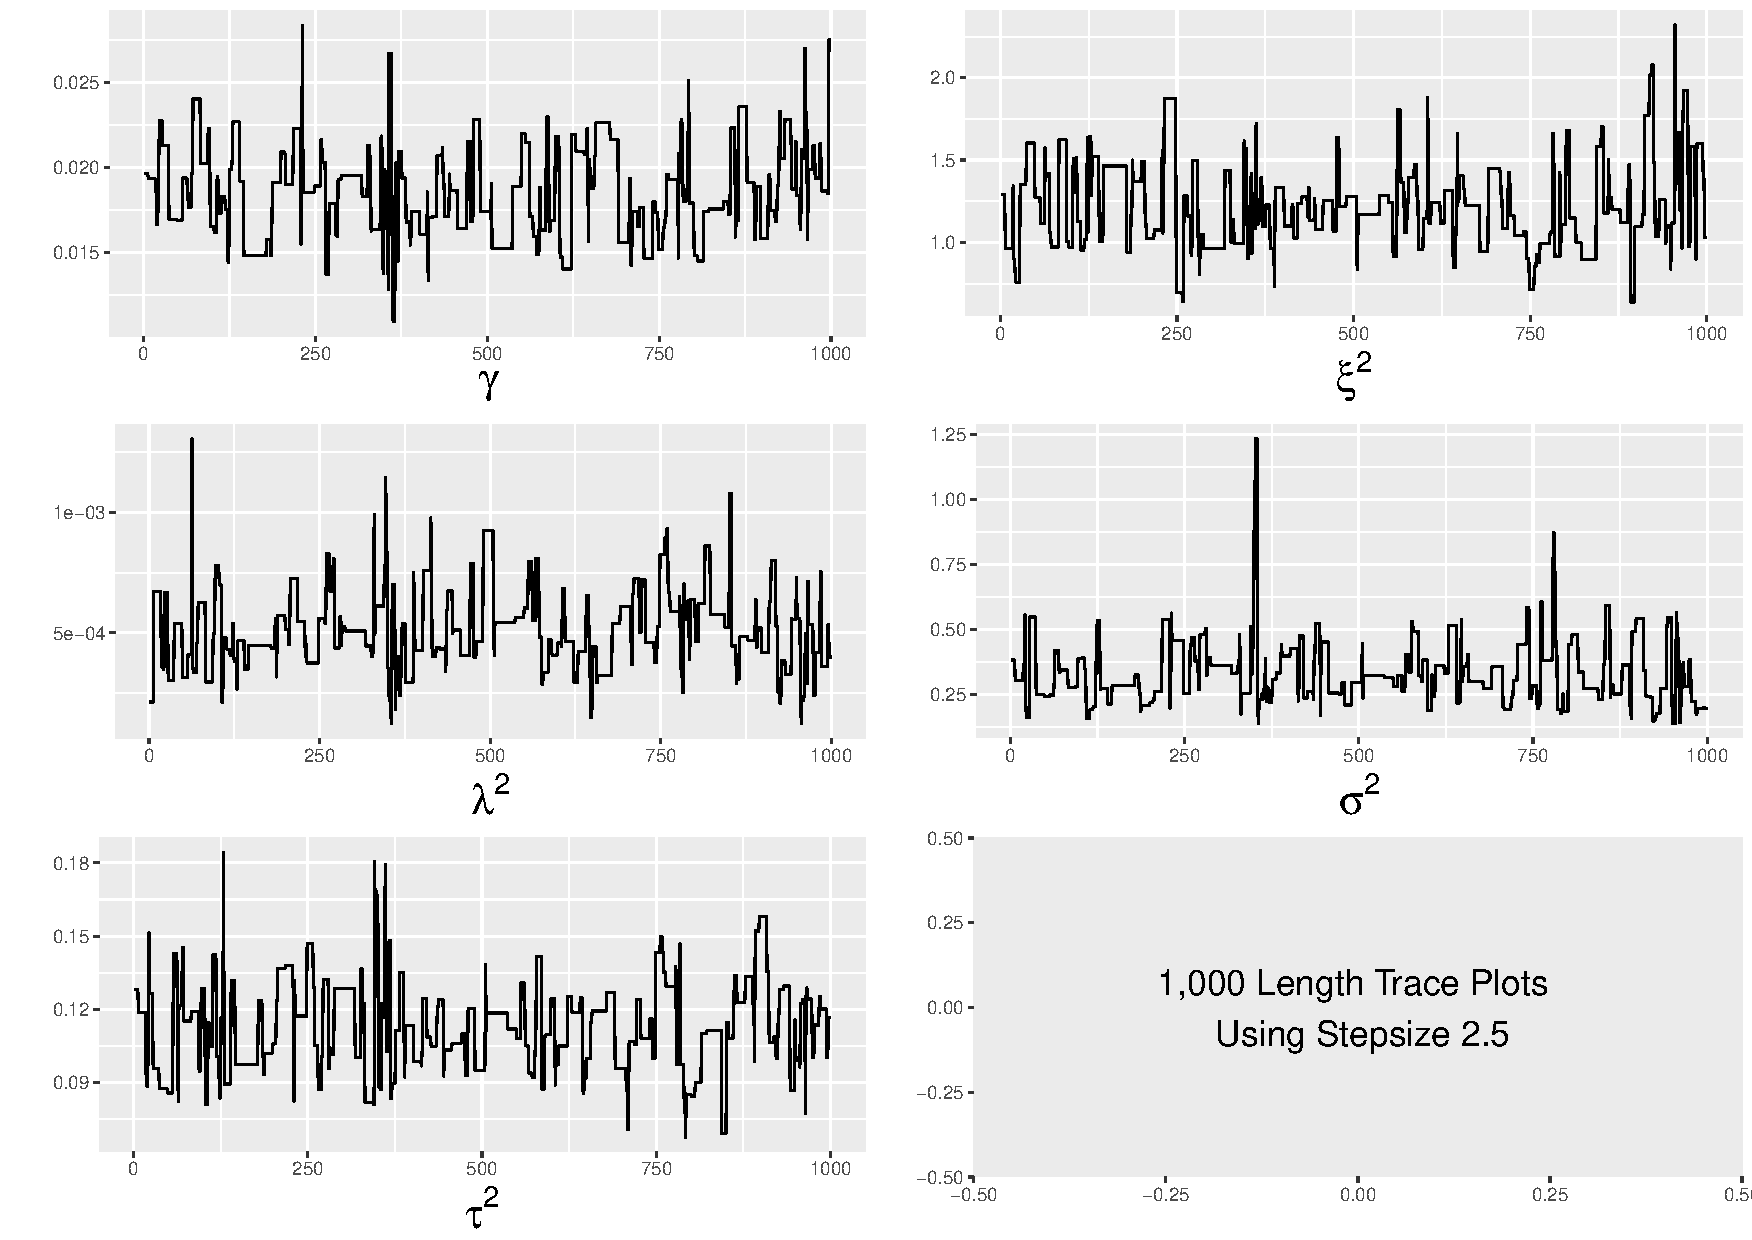
\includegraphics[width=8cm,height=5cm]{Chapters/05MCMCOU/plots/gg1k5chain.pdf}
%%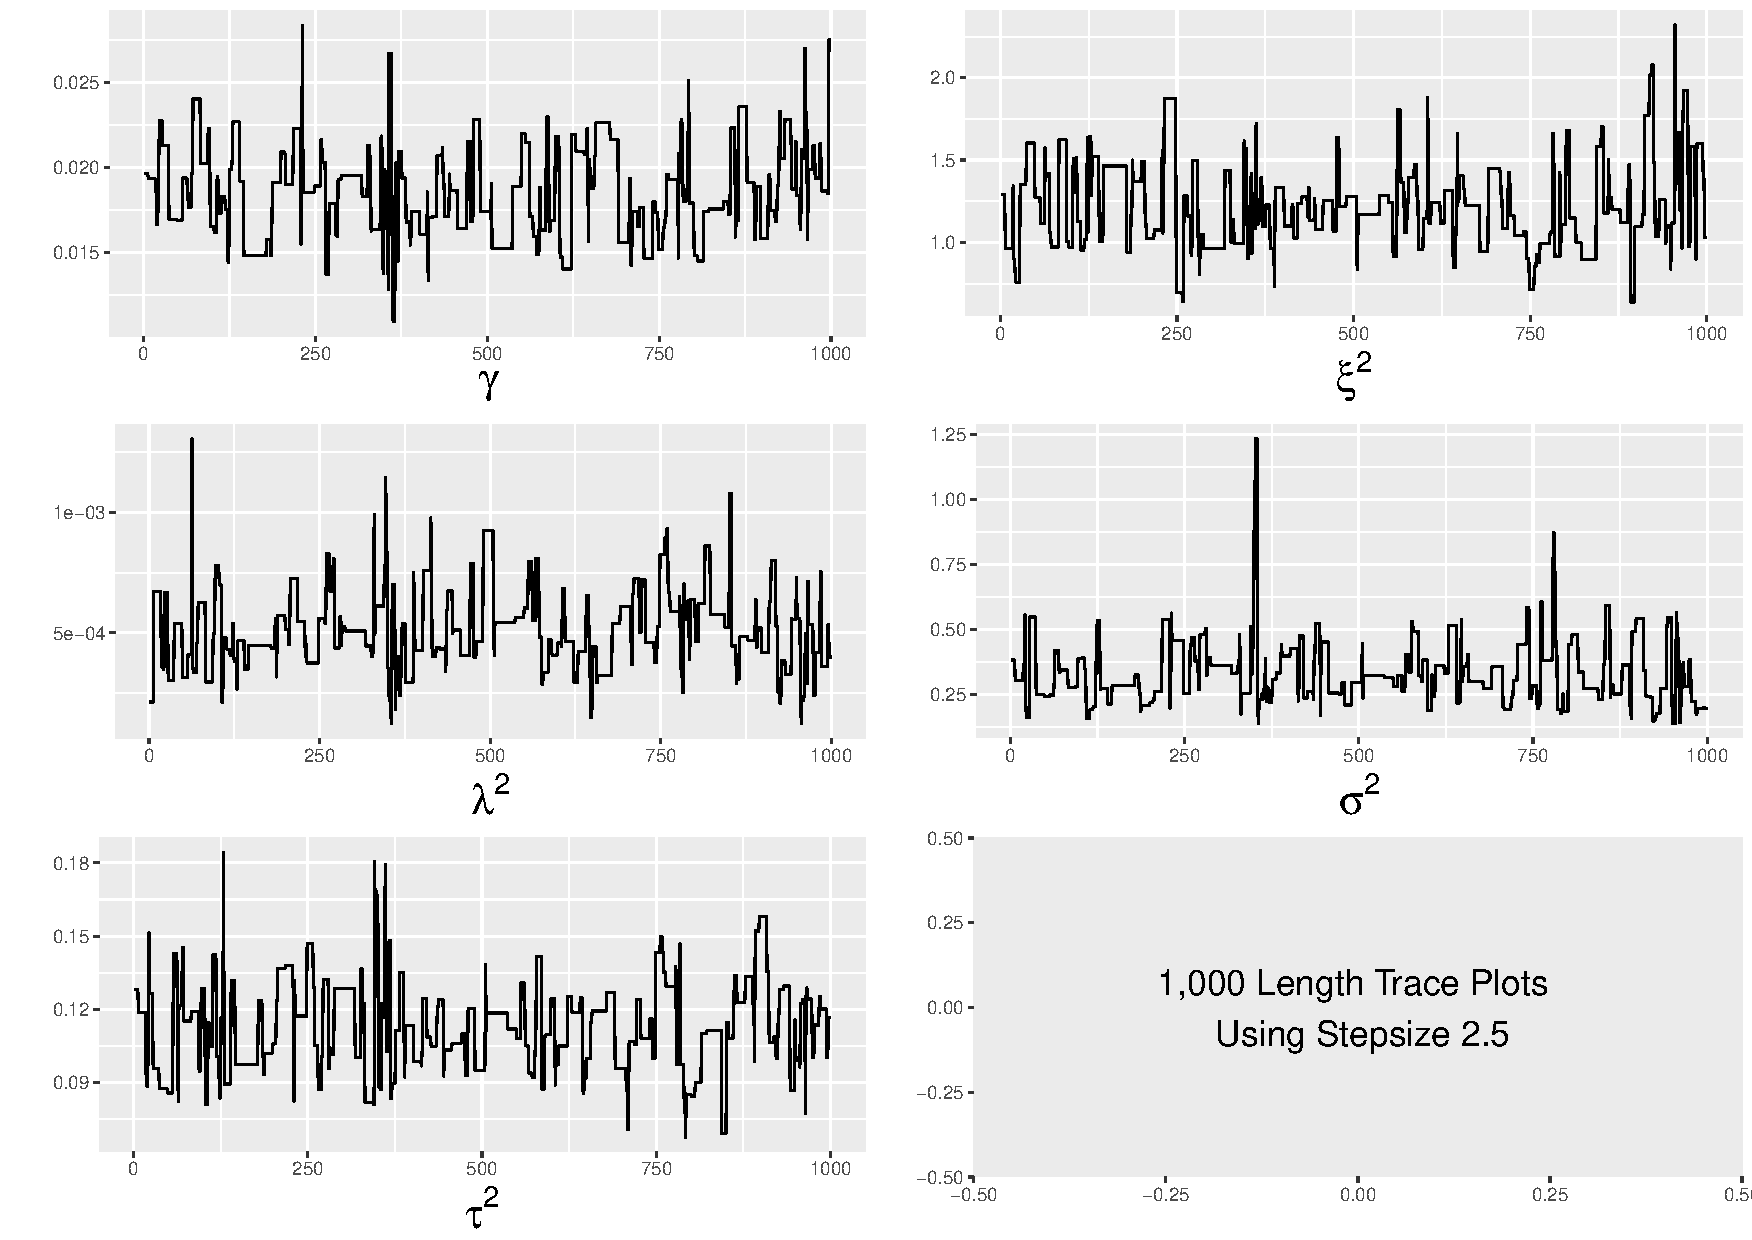
\includegraphics[width=8cm,height=5cm]{Chapters/05MCMCOU/plots/gg1k5chain.pdf}
%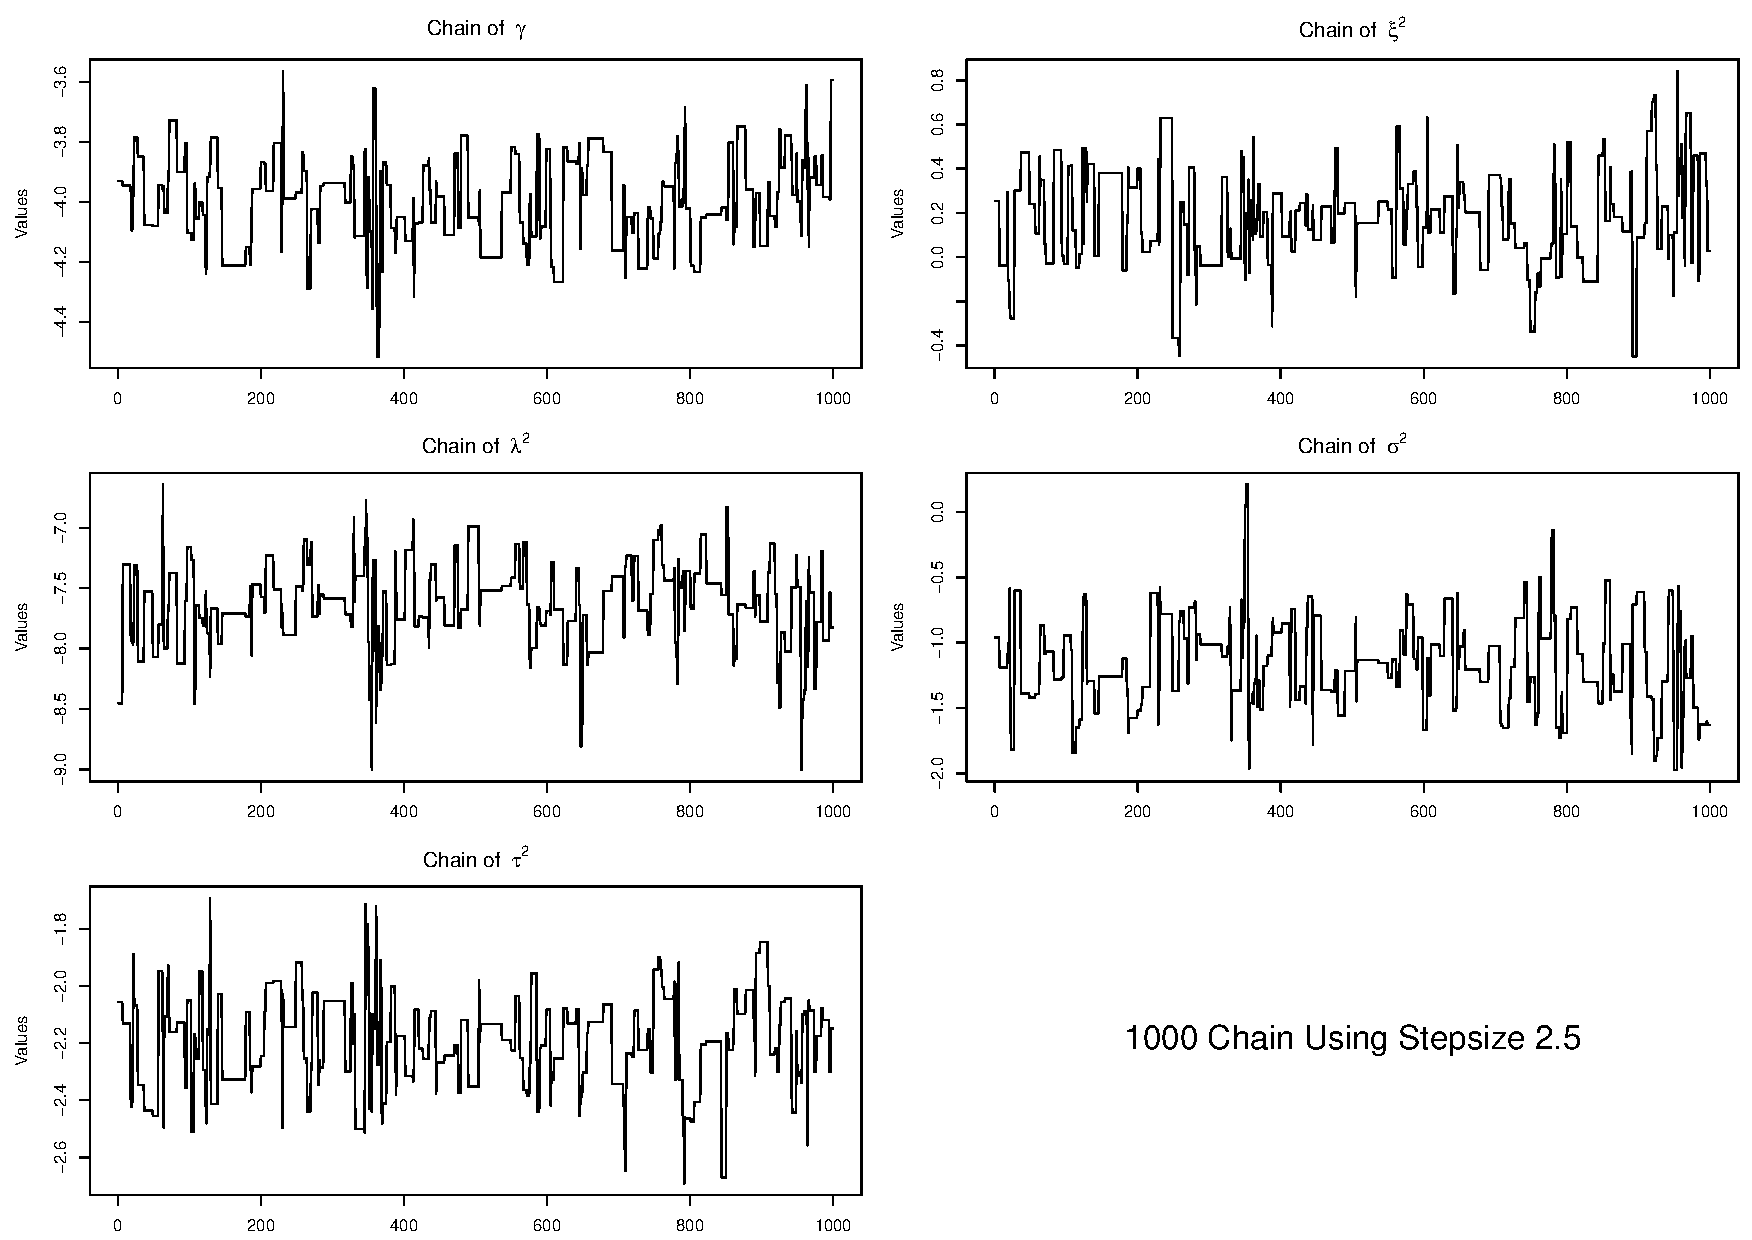
\includegraphics[width=8cm,height=5cm]{Chapters/05MCMCOU/plots/1k5chain.pdf}
%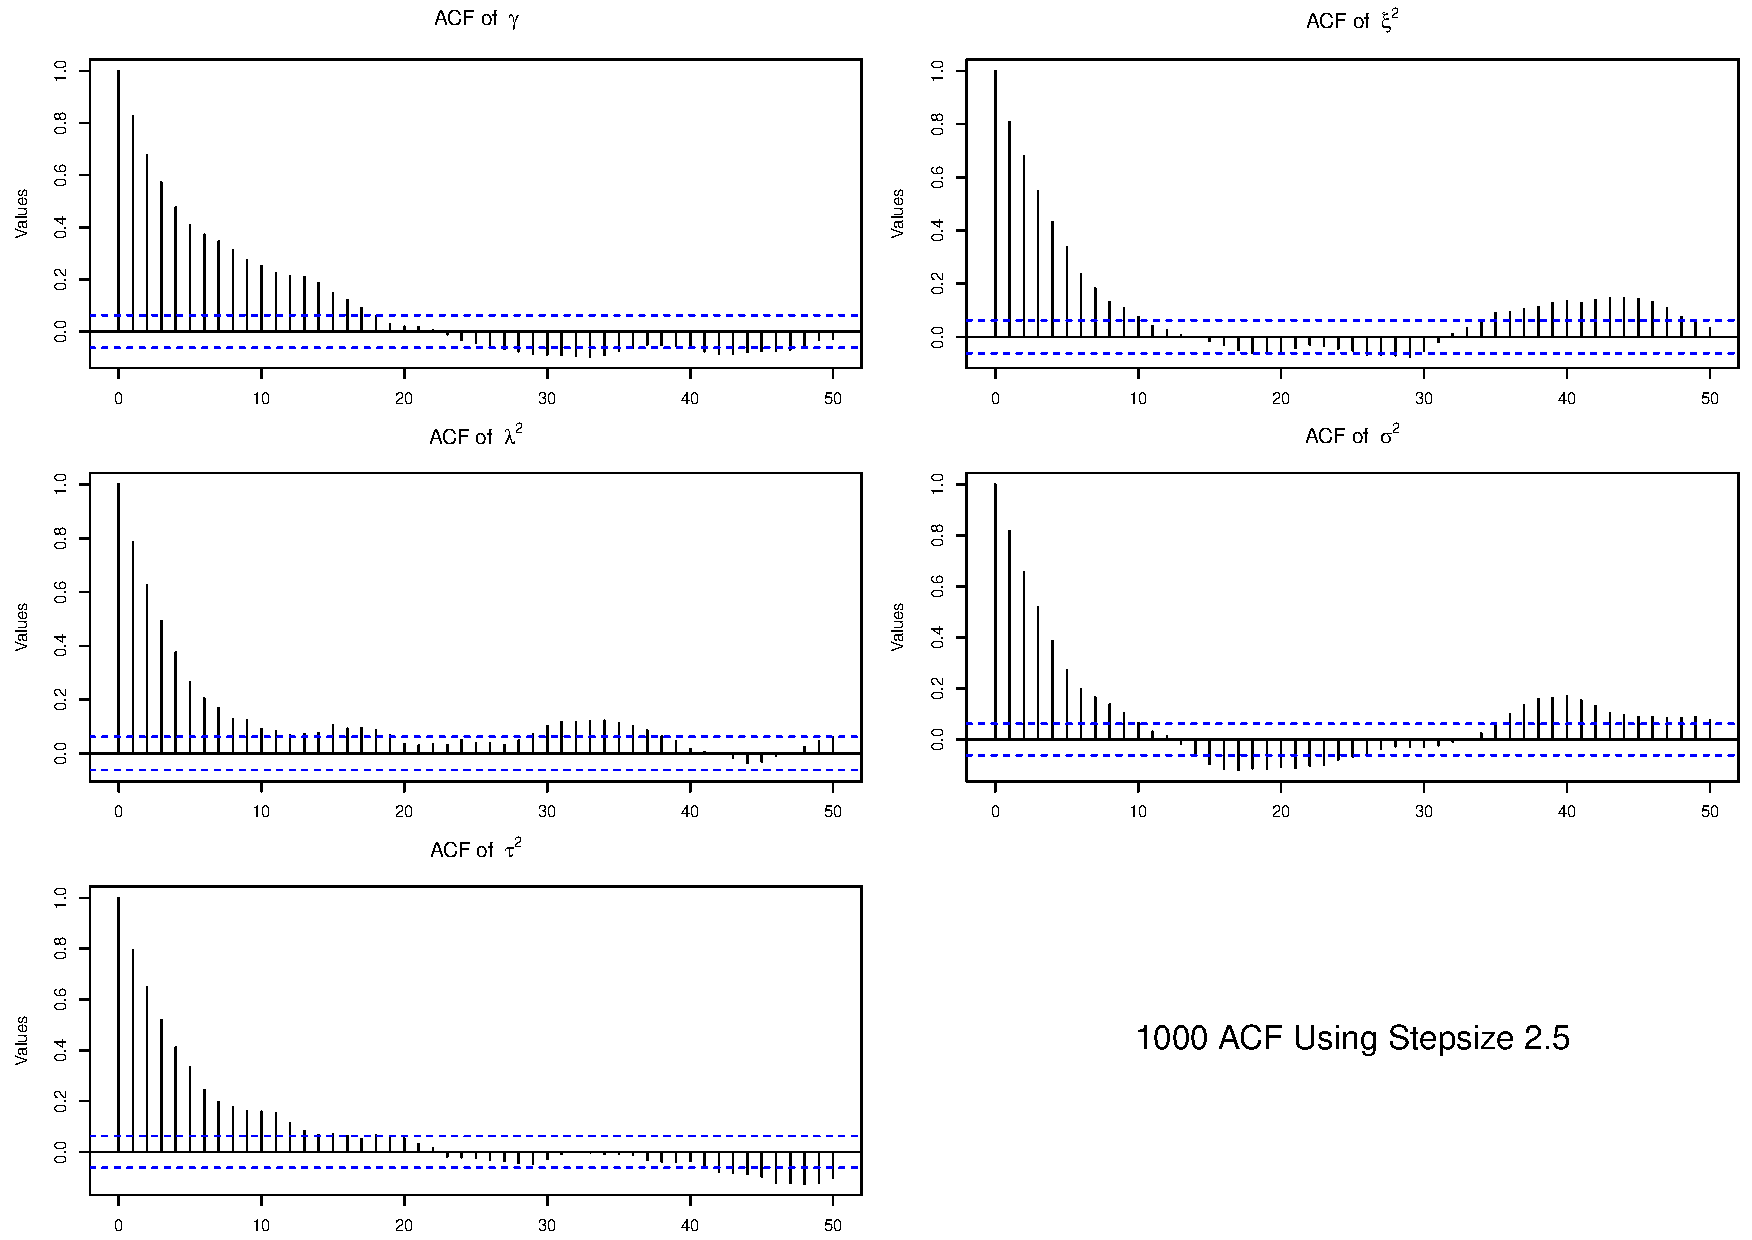
\includegraphics[width=8cm,height=5cm]{Chapters/05MCMCOU/plots/1k5acf.pdf}
%%\includegraphics[width=8cm,height=5cm]{Chapters/05MCMCOU/plots/1k8chain.pdf}
%%\includegraphics[width=8cm,height=5cm]{Chapters/05MCMCOU/plots/1k8acf.pdf}
%\caption{Running the same amount of time and taking the same length of data, the larger step size with the highest ESSUT value generates more effective samples and has a lower correlation. }\label{1koutof8kfigures}
%\end{figure}

\begin{figure}[h]
\centering
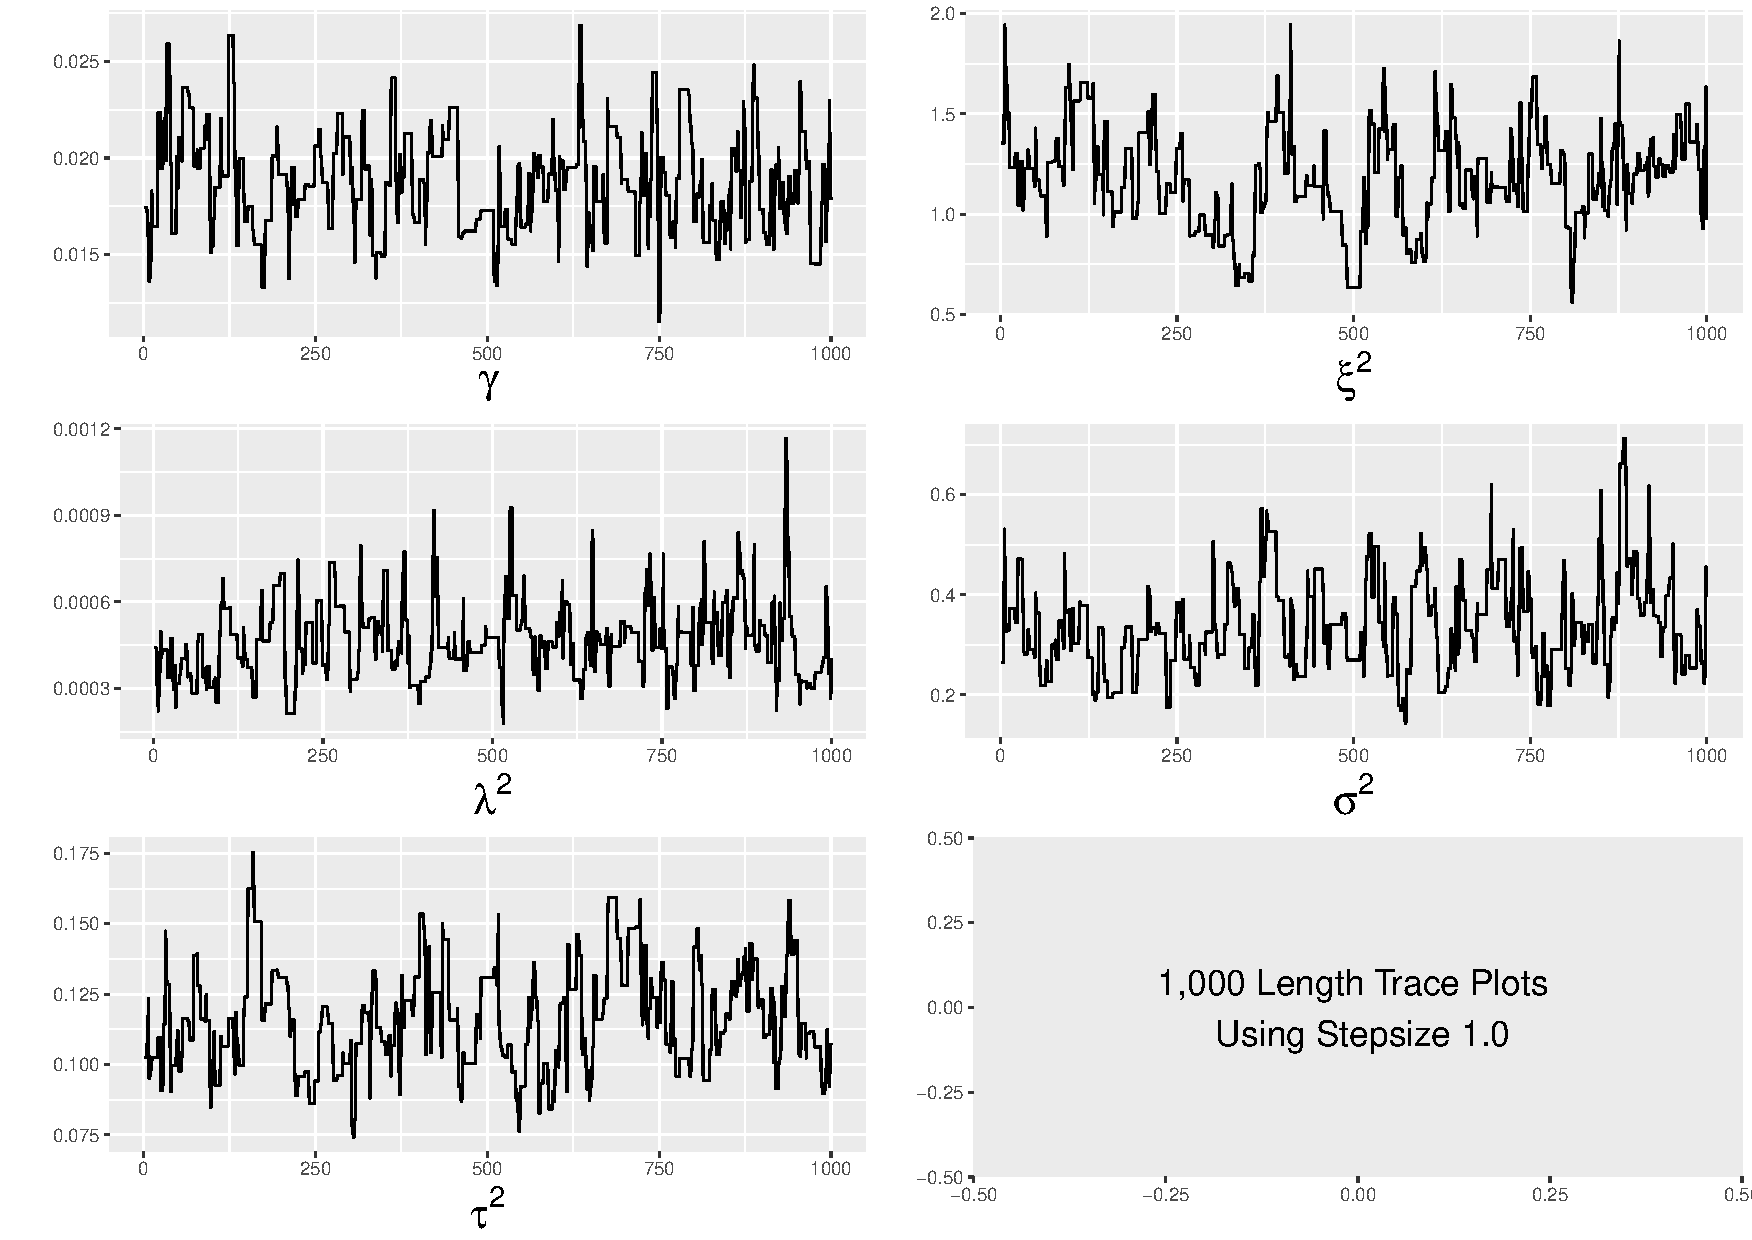
\includegraphics[width=0.45\textwidth,height=5cm]{Chapters/05MCMCOU/plots/gg1k1chain.pdf}
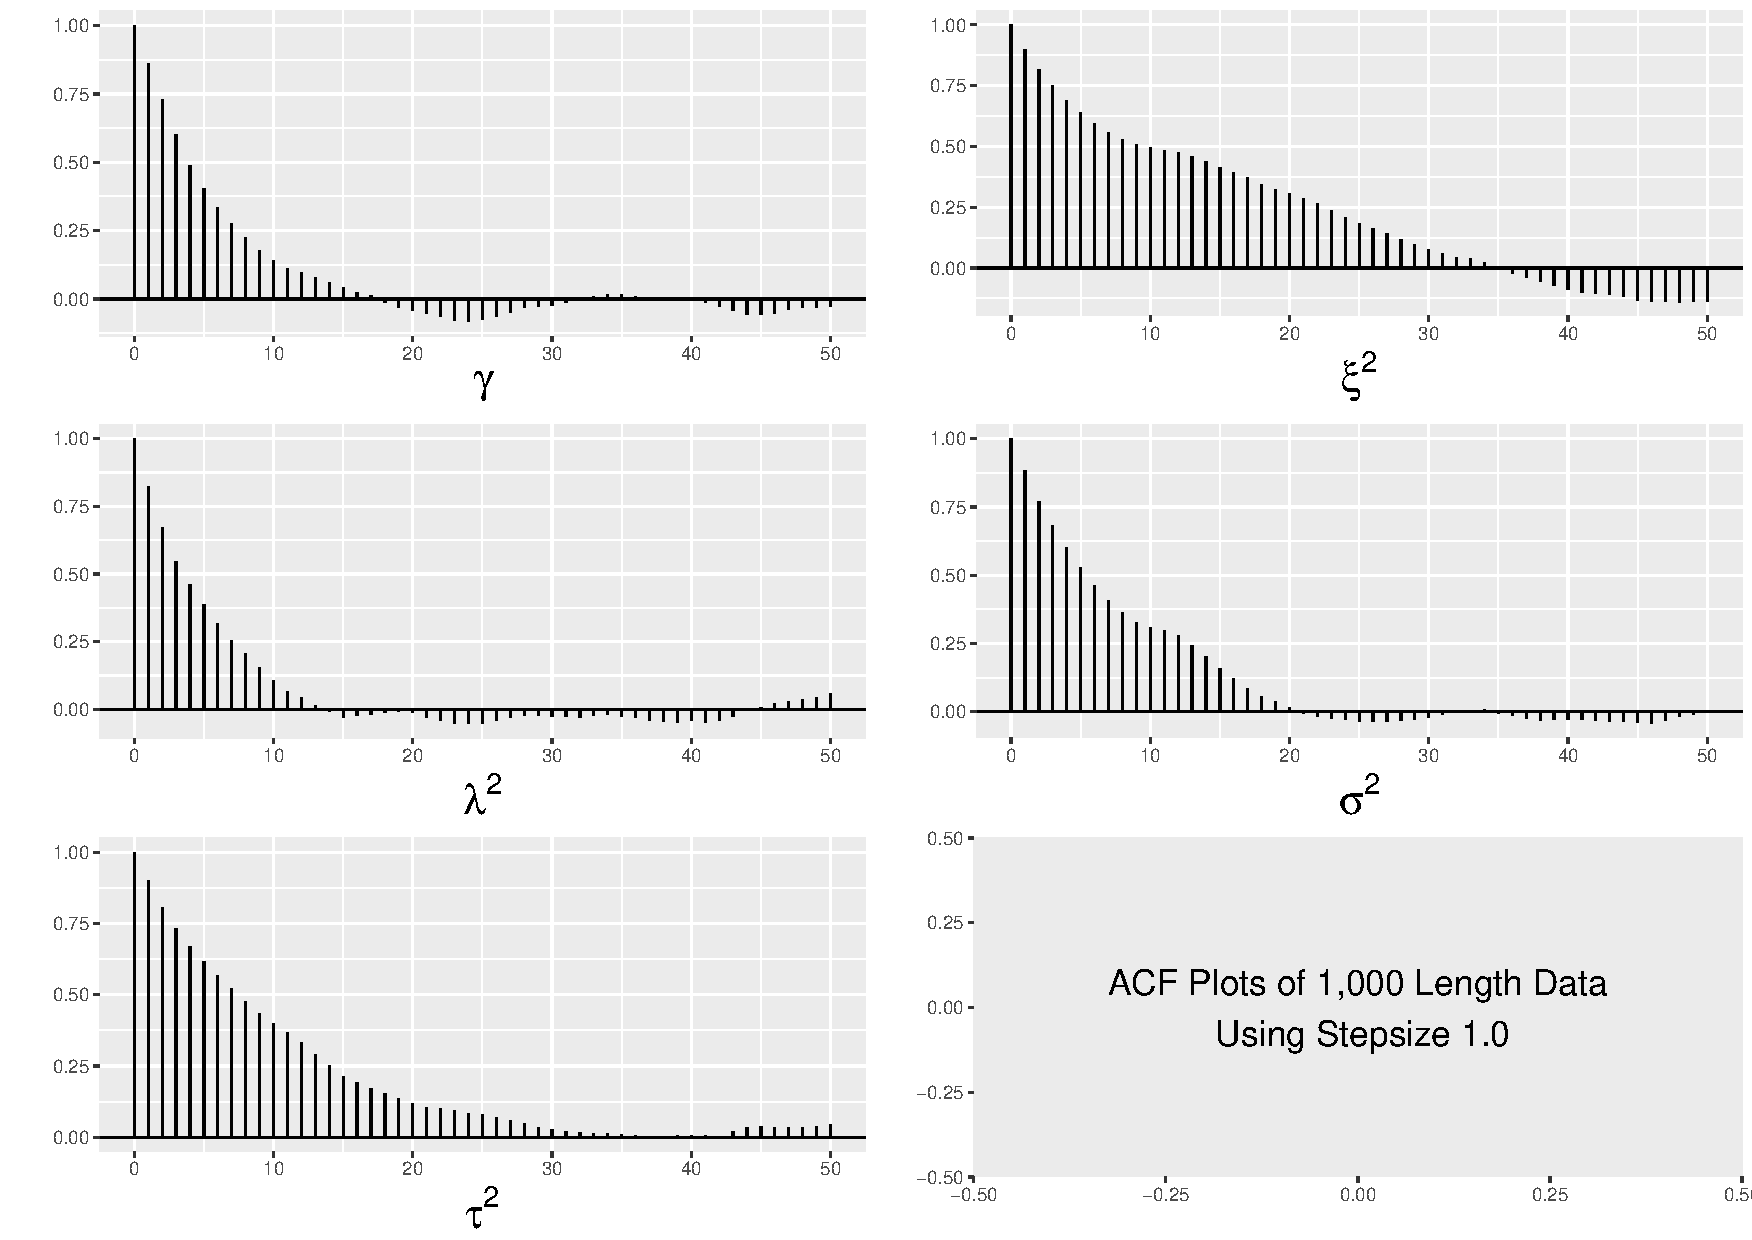
\includegraphics[width=0.45\textwidth,height=5cm]{Chapters/05MCMCOU/plots/gg1k1acf.pdf}
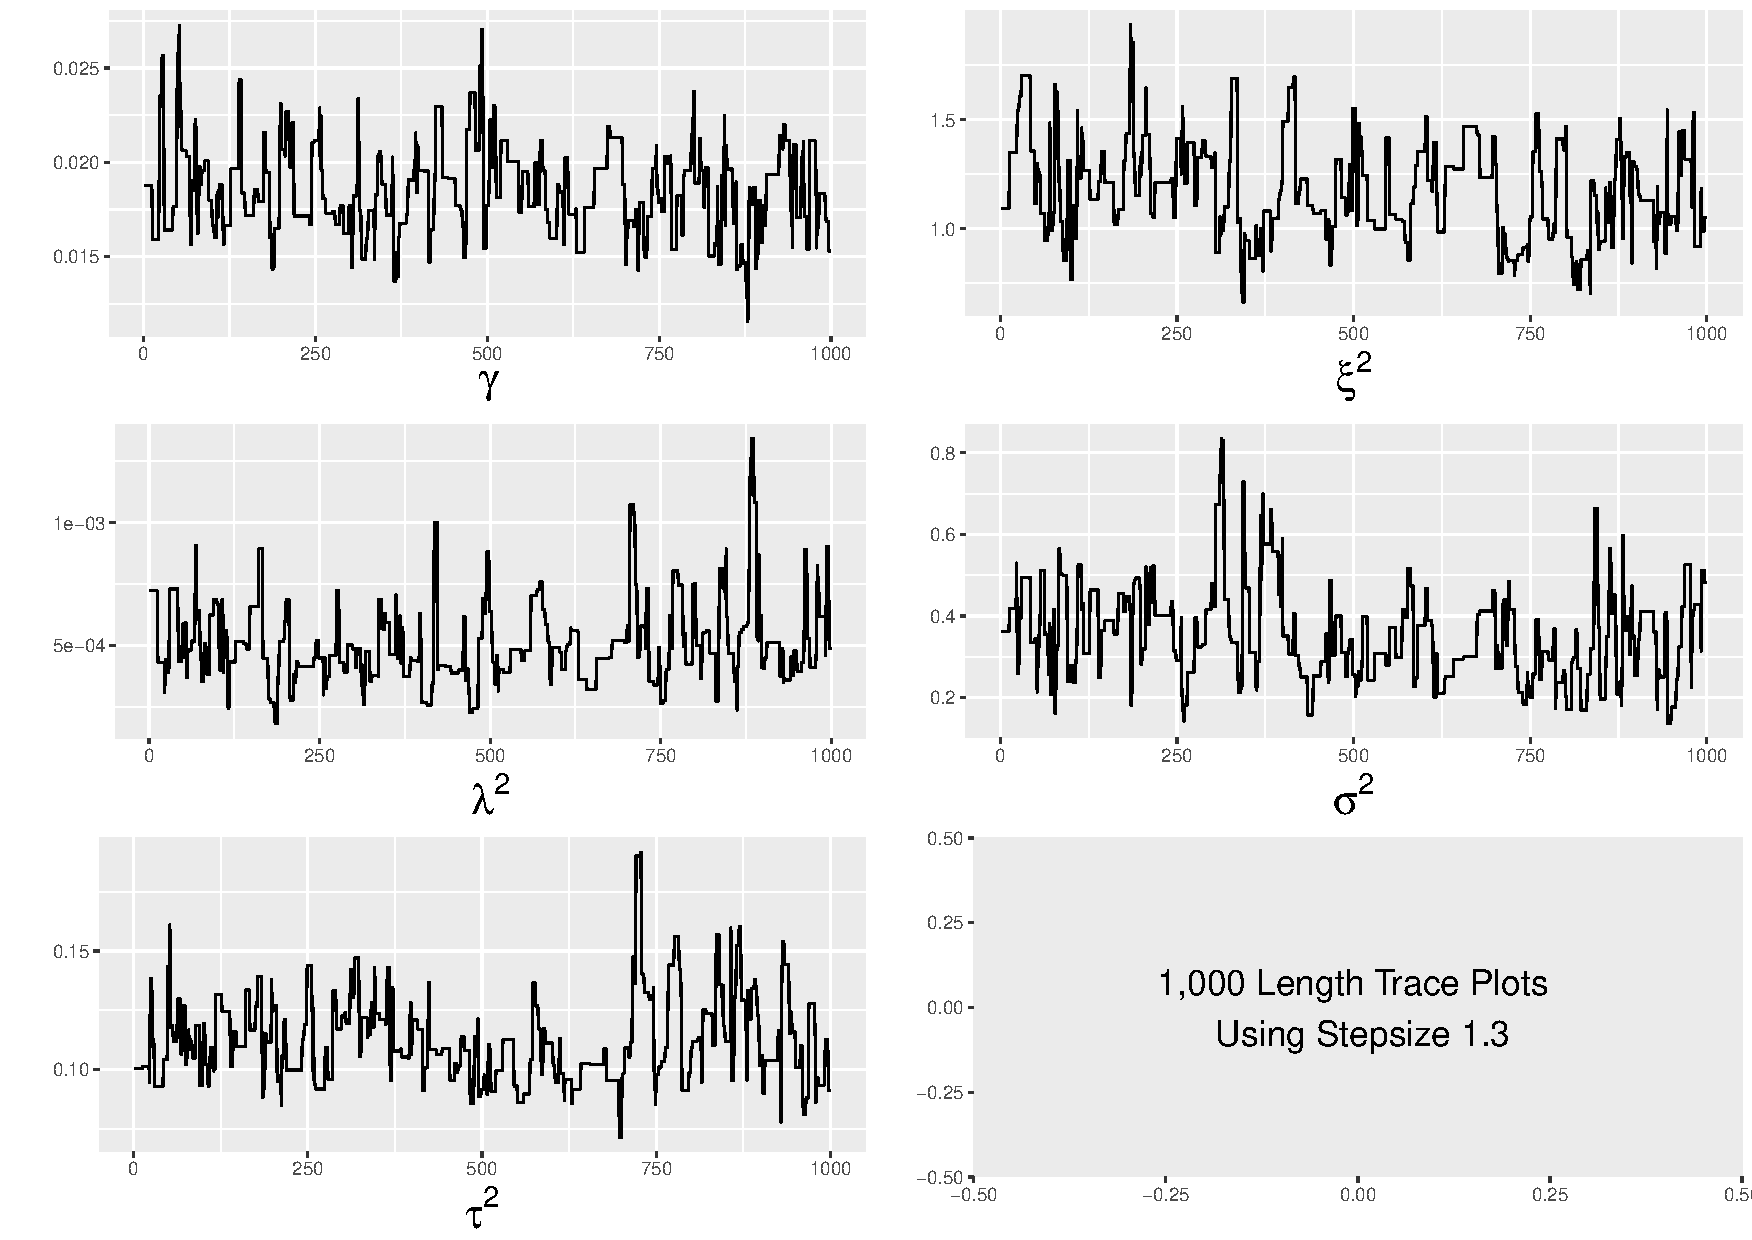
\includegraphics[width=0.45\textwidth,height=5cm]{Chapters/05MCMCOU/plots/gg1k13chain.pdf}
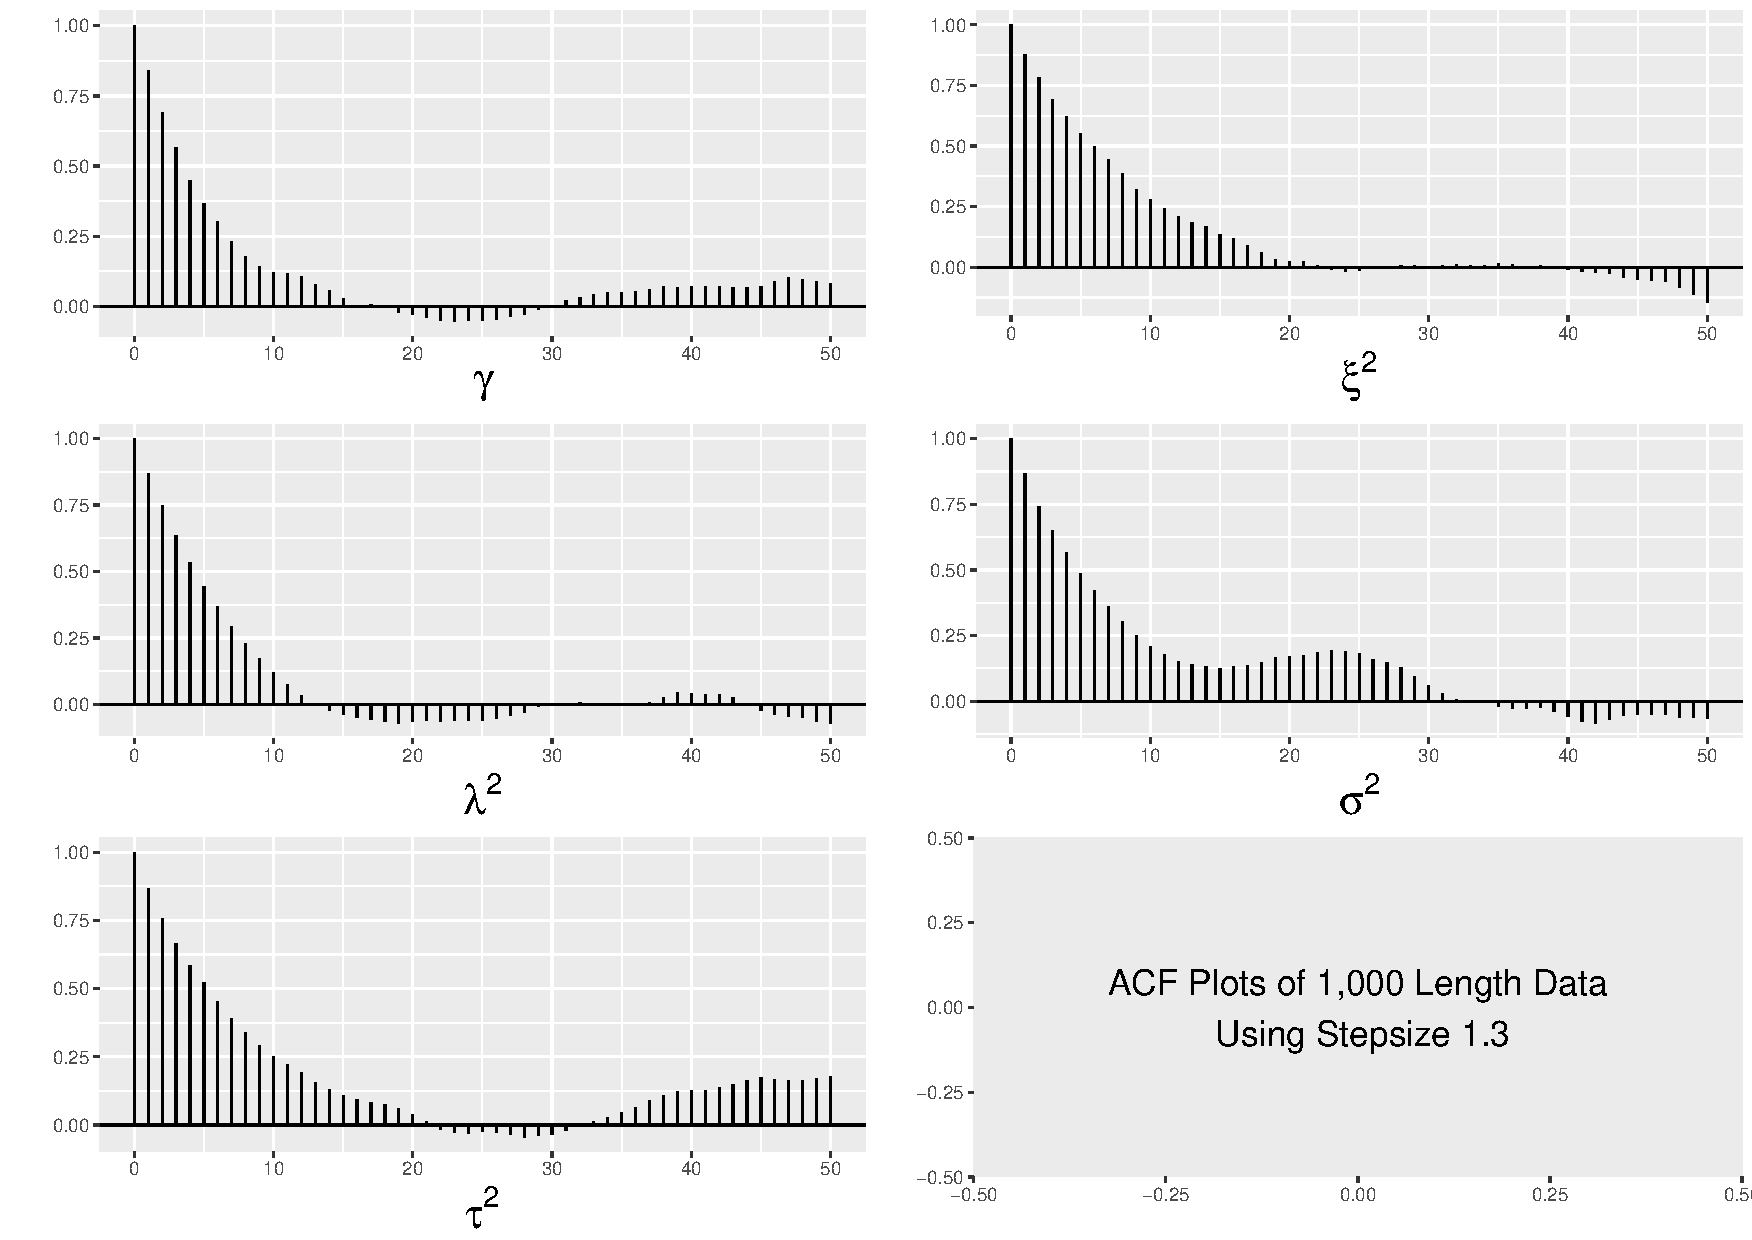
\includegraphics[width=0.45\textwidth,height=5cm]{Chapters/05MCMCOU/plots/gg1k13acf.pdf}
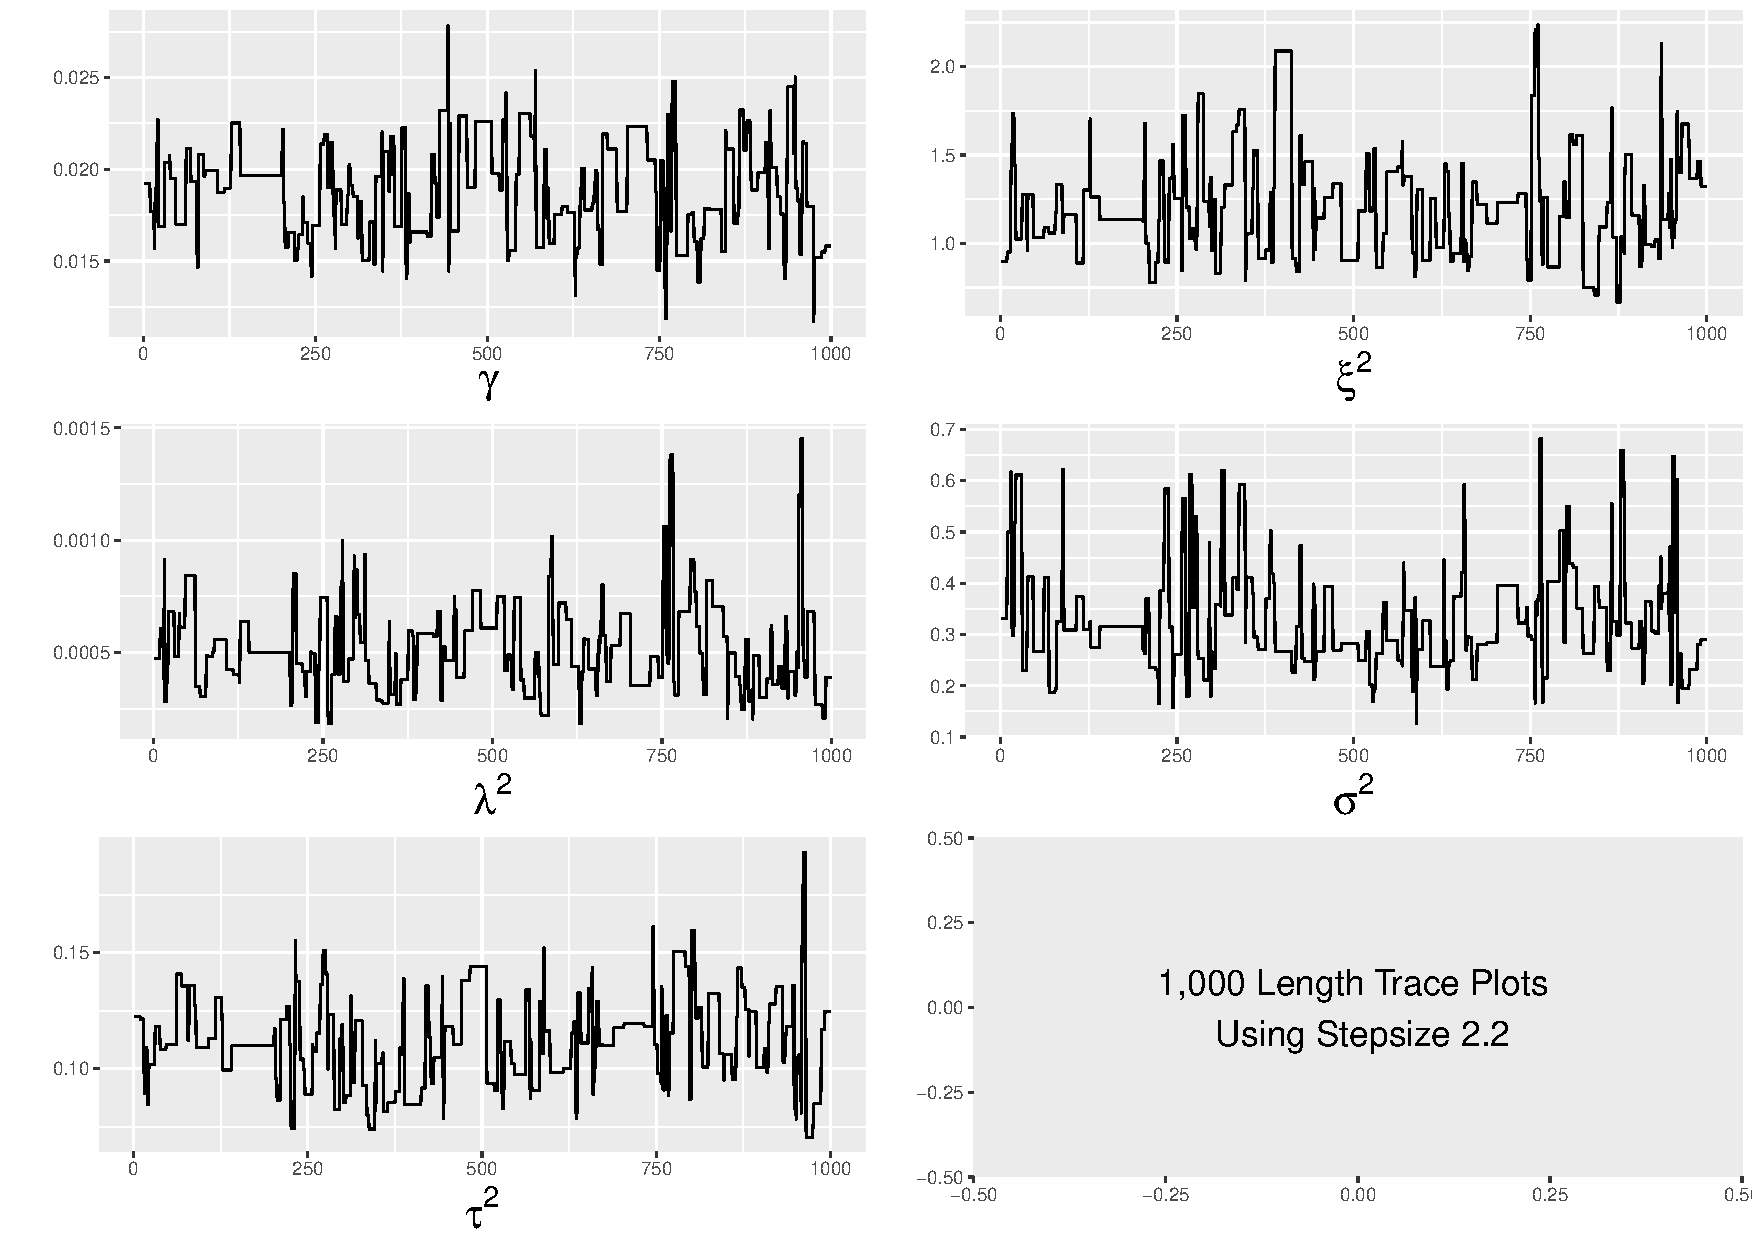
\includegraphics[width=0.45\textwidth,height=5cm]{Chapters/05MCMCOU/plots/gg1k22chain.pdf}
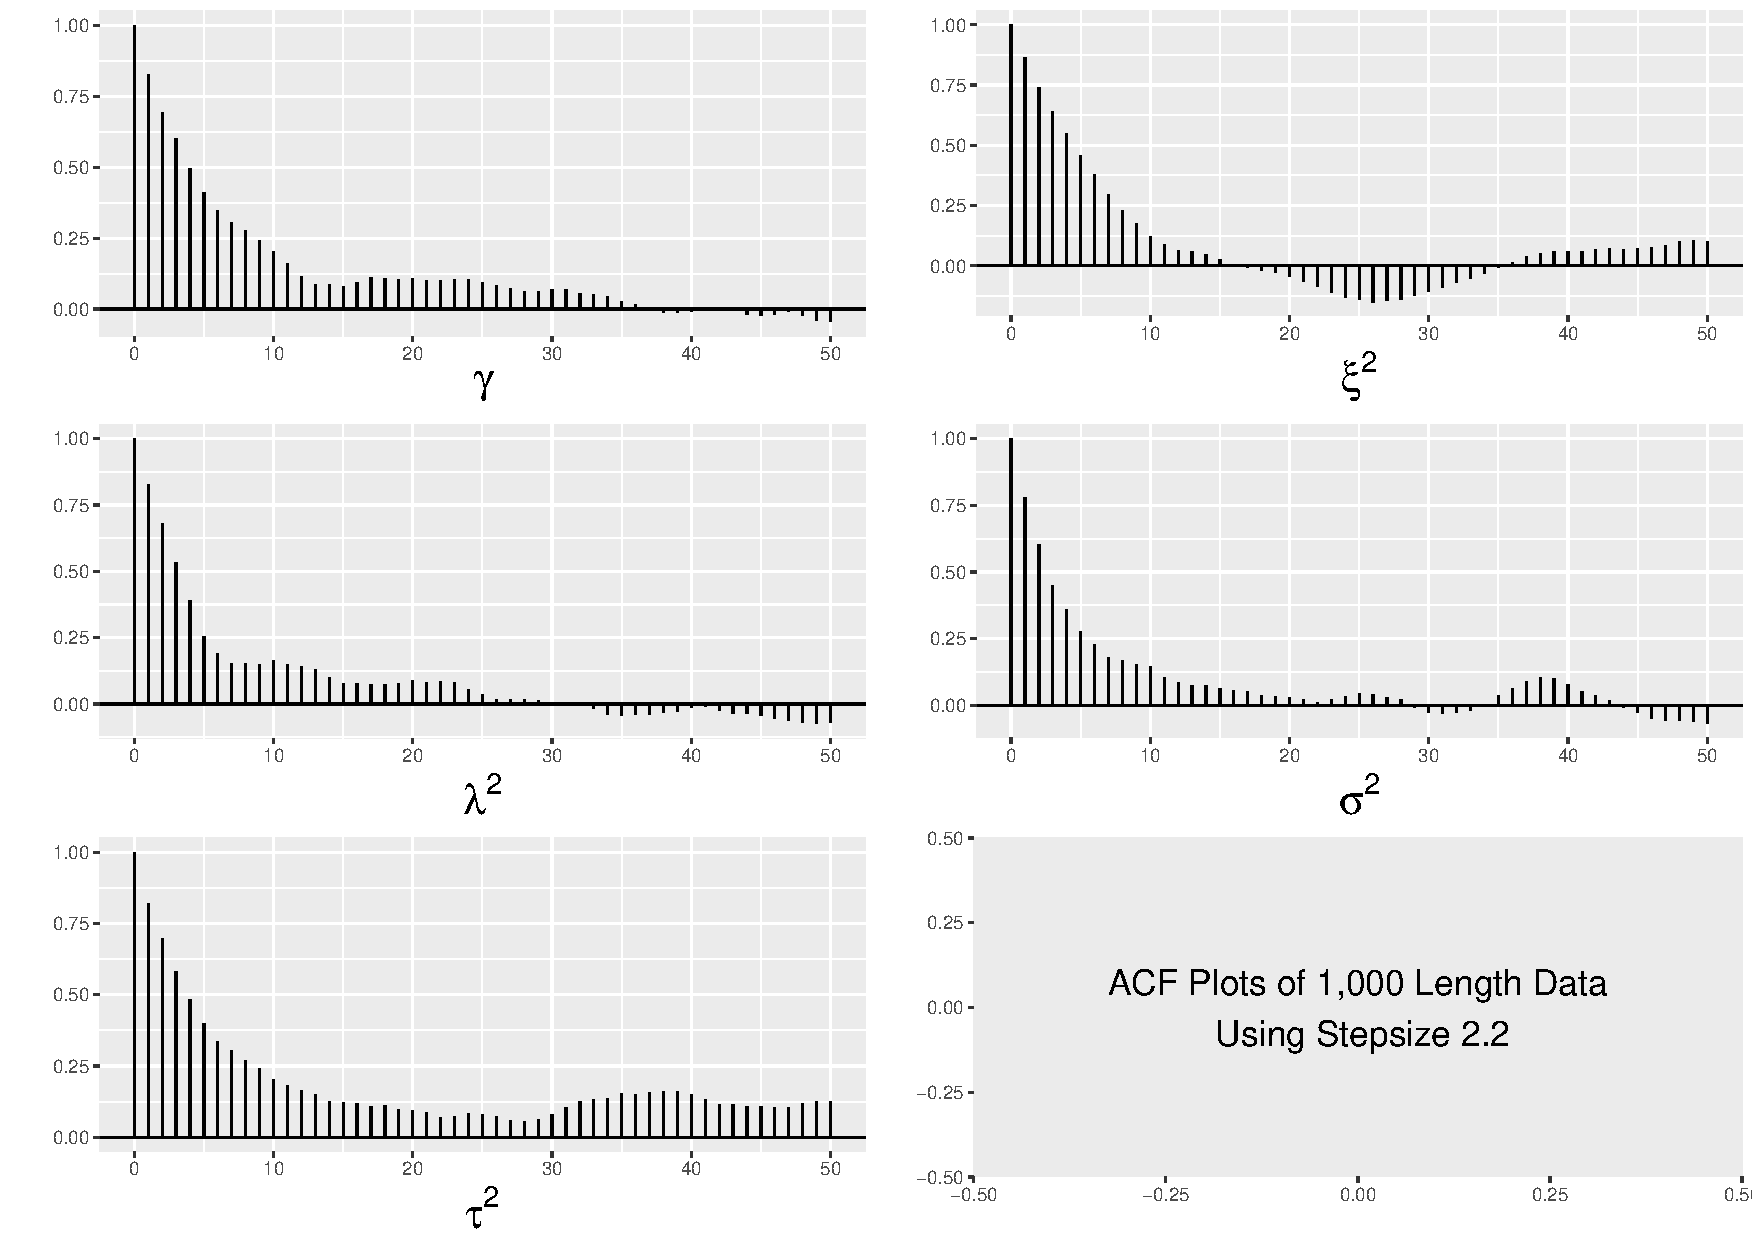
\includegraphics[width=0.45\textwidth,height=5cm]{Chapters/05MCMCOU/plots/gg1k22acf.pdf}
\end{figure}
\begin{figure}[h]\ContinuedFloat
\centering
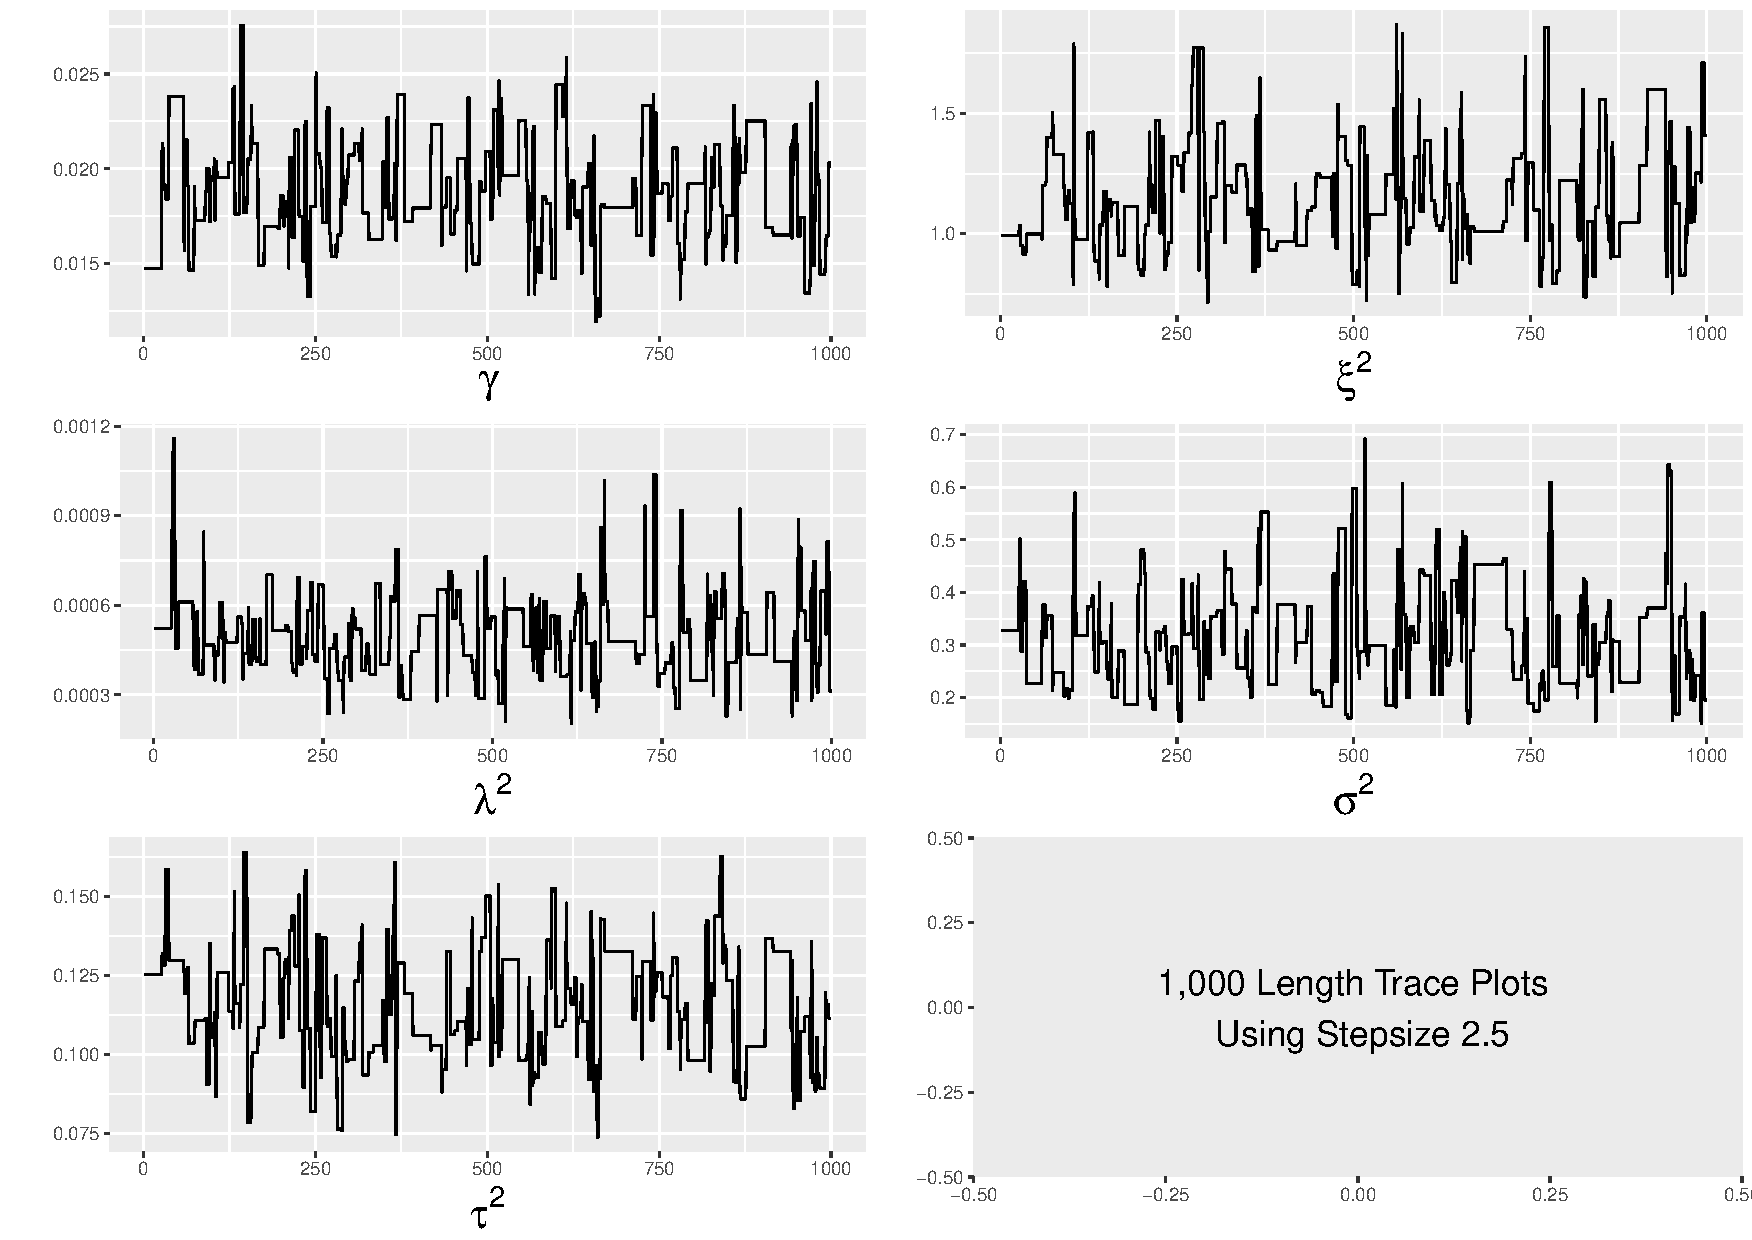
\includegraphics[width=0.45\textwidth,height=5cm]{Chapters/05MCMCOU/plots/gg1k25chain.pdf}
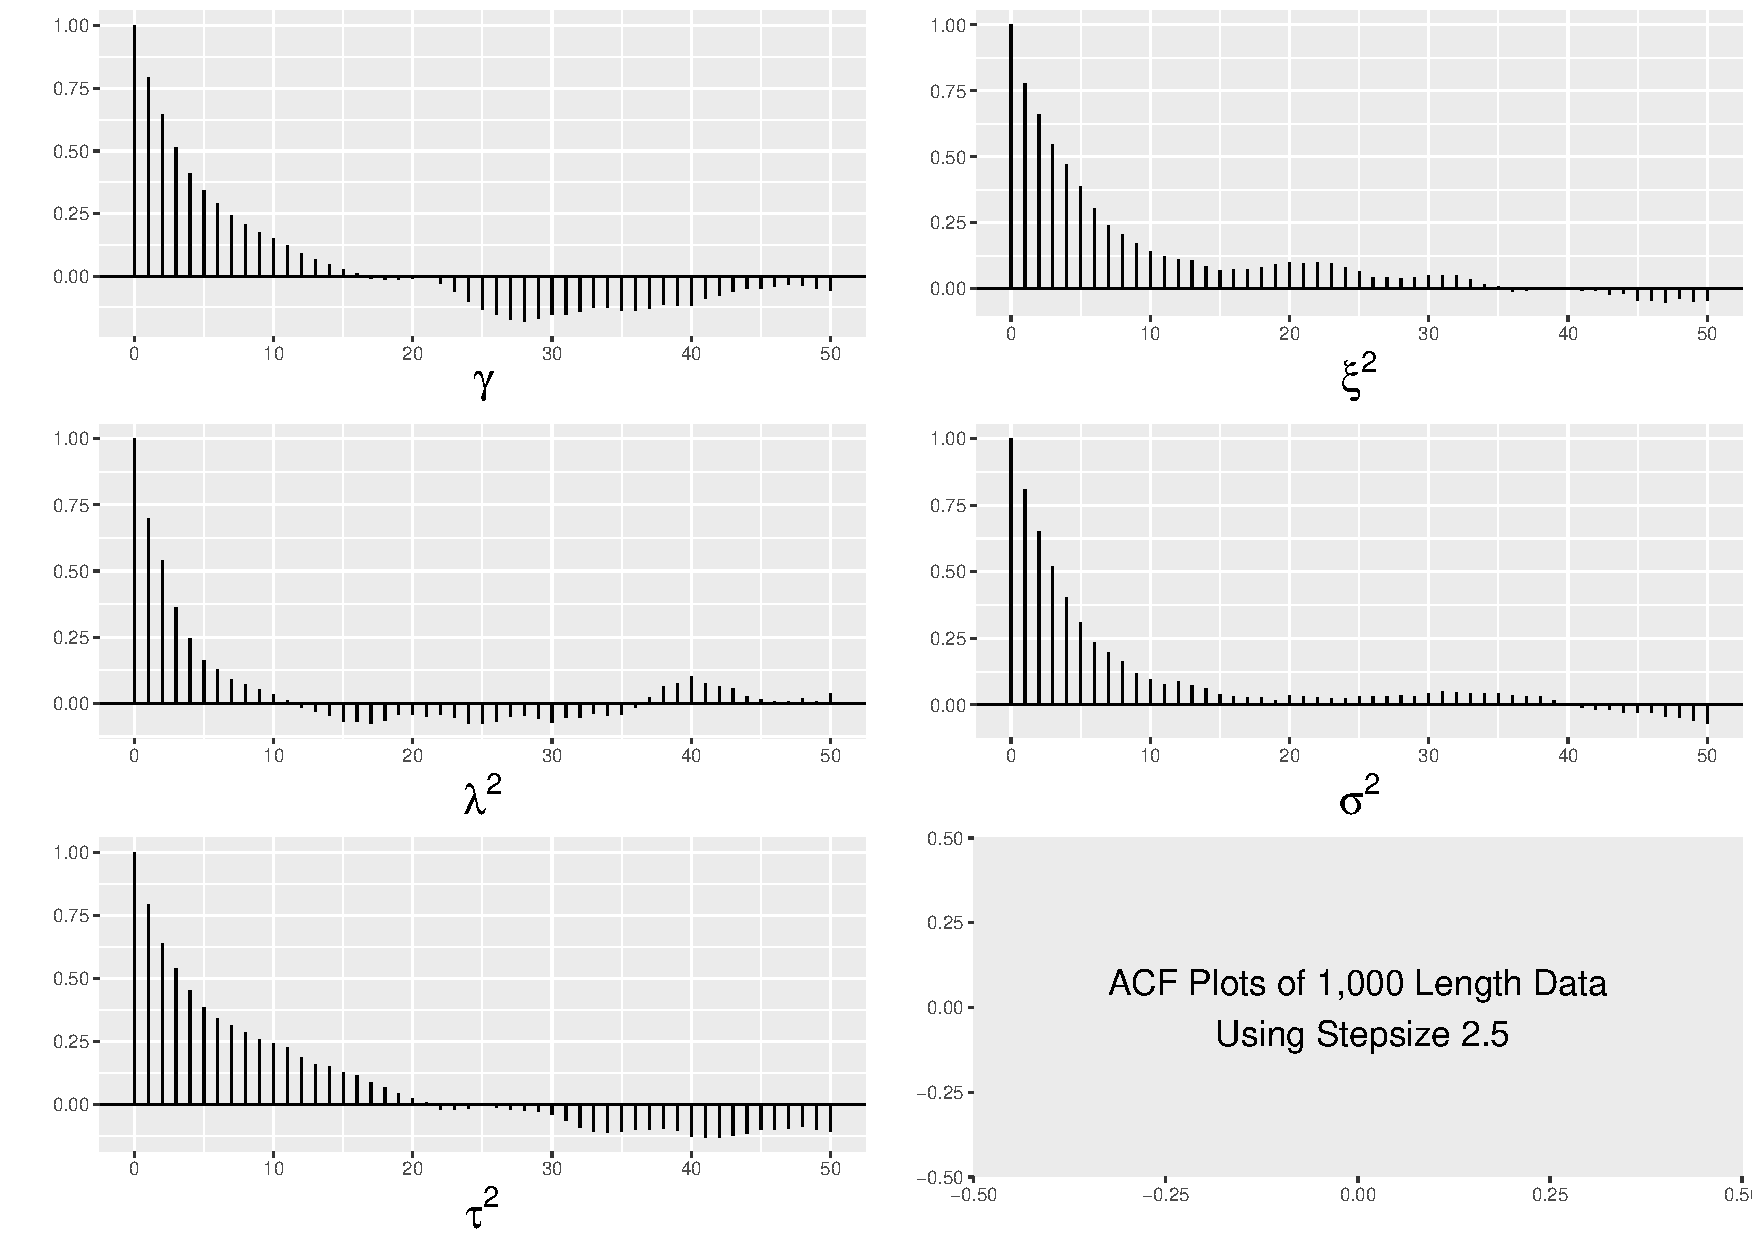
\includegraphics[width=0.45\textwidth,height=5cm]{Chapters/05MCMCOU/plots/gg1k25acf.pdf}
\caption{Running the same amount of time and taking the same length of data, the step size $\epsilon=2.5$ returns the highest ESSUT value and generates more effective samples in a lower correlated relationship. }\label{1koutof8kfigures}
\end{figure}



\clearpage

\subsection*{Comparing Estimation with Different Length of Data }


\begin{figure}[h]
\centering
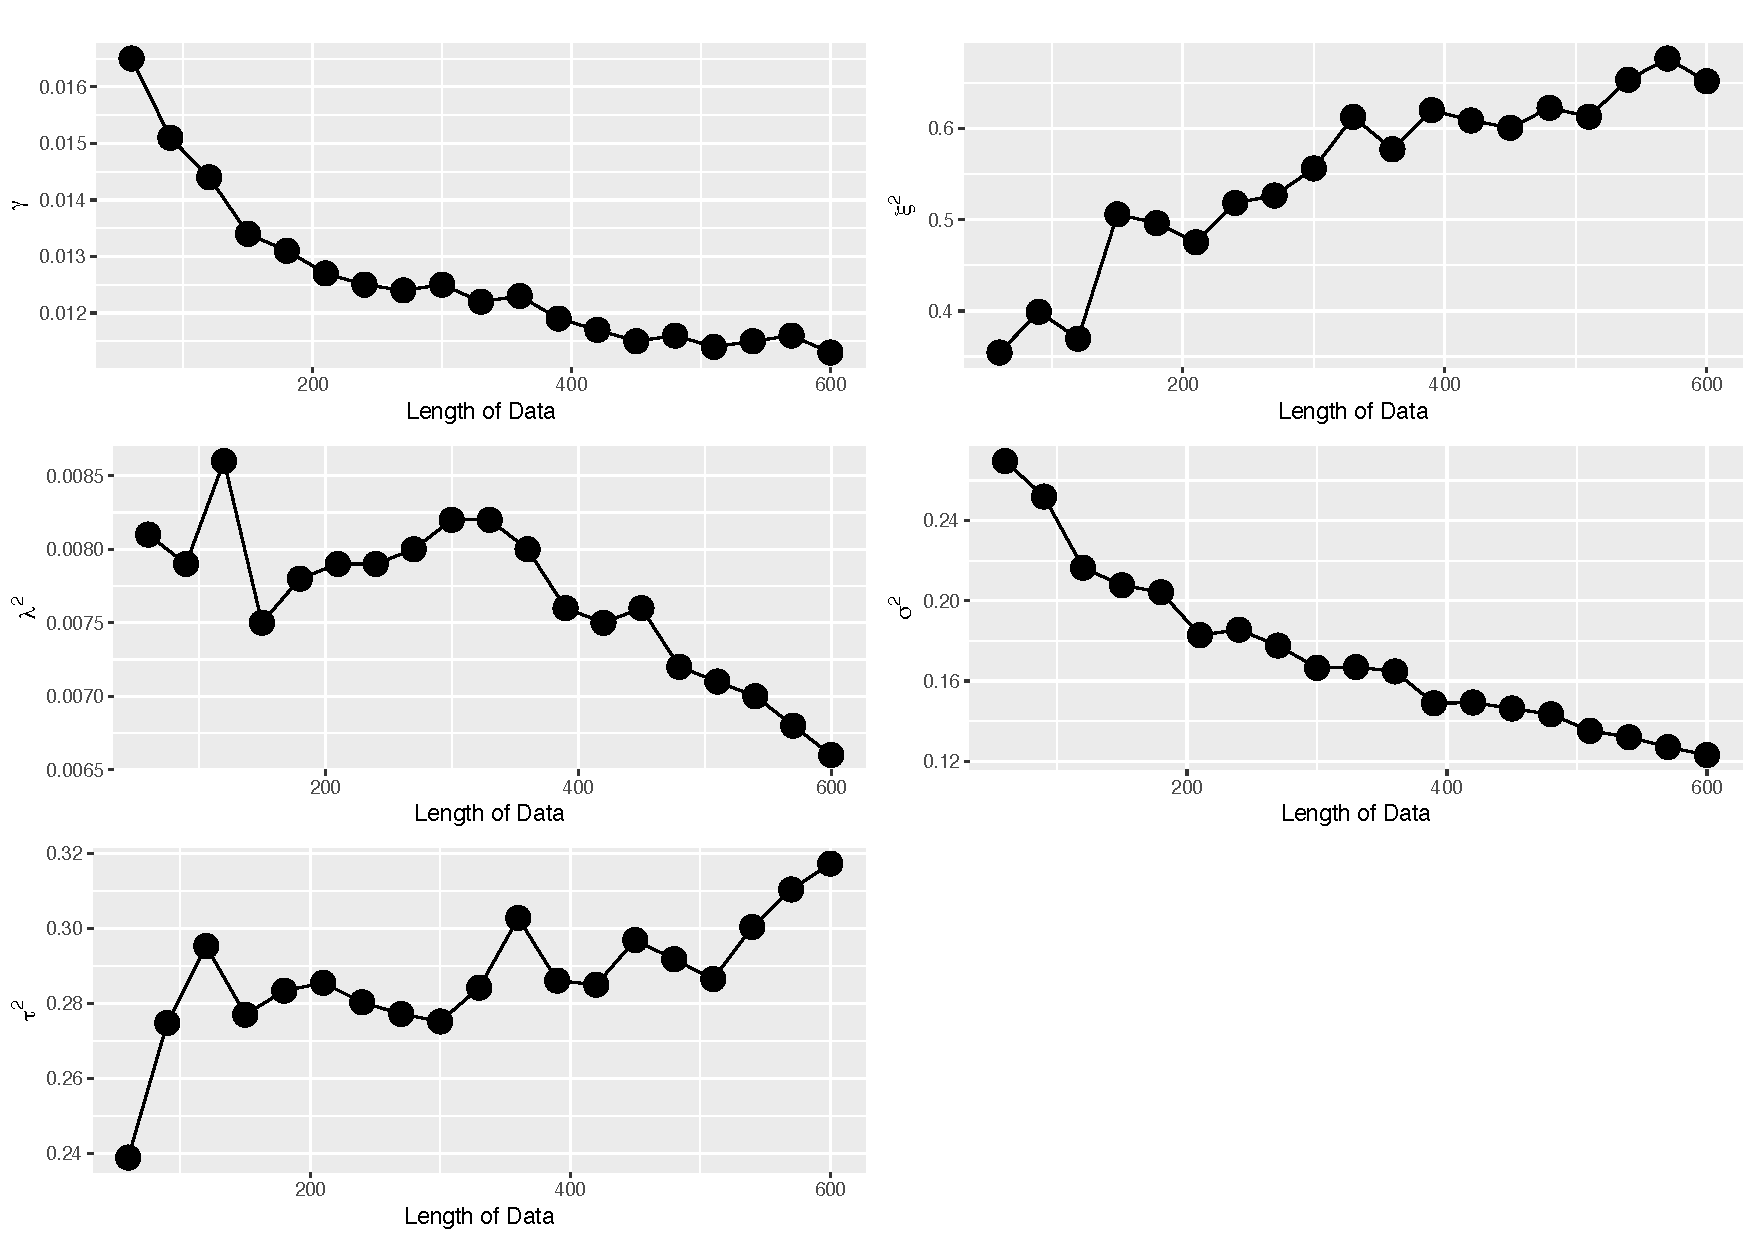
\includegraphics[width=\textwidth,height=0.5\textheight]{Chapters/05MCMCOU/plots/realdatalengthcompare.pdf}
\caption{Impacts of data length on optimal parameter. There is an obvious trend on the estimation against length of data in the estimation process. }
\end{figure}



\begin{landscape}
%\begin{table}[h]
%\centering
%\caption{Parameter estimation by running the whole surface learning and DA-MH processes with different length of data}
%\begin{tabular}{|l|l|l|l|l|l|l|l|l|l|l|l|l|}
%\hline
%\textbf{Length} & \textbf{Time} & $\gamma$ & $\xi$ & $\lambda$ & $\sigma$ & $\tau$ & $\alpha_1$ & $\alpha_2$ &$x$ & $v_x$ &$y$&$v_y$\\ \hline
%\textbf{Obs}    & -             & -              & -           & -             & -              & -            & -           & -           & -339.0569  & 0.0414  & -100.2065  & 1.1825    \\ \hline
%\textbf{600}    & 80.03         & 0.0113         & 0.8076      & 0.0813        & 0.3509         & 0.5633       & 0.0536      & 0.7873      & -339.0868  & 0.4331      & -100.1498  & -0.7498     \\ \hline
%\textbf{550}    & 82.01         & 0.0116         & 0.8369      & 0.0828        & 0.3606         & 0.5492       & 0.0574      & 0.7038      & -339.0878  & 0.4253      & -100.1456  & -0.7231     \\ \hline
%\textbf{500}    & 79.65         & 0.0115         & 0.7829      & 0.0854        & 0.3698         & 0.5412       & 0.0564      & 0.8121      & -339.0905  & 0.4397      & -100.1391  & -0.7464     \\ \hline
%\textbf{450}    & 77.50         & 0.0115         & 0.7752      & 0.0871        & 0.3825         & 0.5449       & 0.0580      & 0.7931      & -339.0924  & 0.4432      & -100.1348  & -0.7521     \\ \hline
%\textbf{400}    & 76.11         & 0.0120         & 0.7760      & 0.0879        & 0.3886         & 0.5347       & 0.0658      & 0.7781      & -339.0941  & 0.4405      & -100.1298  & -0.7404     \\ \hline
%\textbf{350}    & 75.13         & 0.0122         & 0.7854      & 0.0897        & 0.4034         & 0.5380       & 0.0534      & 0.7341      & -339.0958  & 0.4399      & -100.1254  & -0.7368     \\ \hline
%\textbf{300}    & 73.99         & 0.0125         & 0.7459      & 0.0904        & 0.4081         & 0.5246       & 0.0548      & 0.8212      & -339.0989  & 0.4457      & -100.1174  & -0.7443     \\ \hline
%\textbf{250}    & 71.48         & 0.0123         & 0.7372      & 0.0893        & 0.4282         & 0.5310       & 0.0508      & 0.8346      & -339.1031  & 0.4480      & -100.1102  & -0.7542     \\ \hline
%\textbf{200}    & 68.53         & 0.0129         & 0.6461      & 0.0904        & 0.4338         & 0.5280       & 0.0514      & 0.7510      & -339.1082  & 0.4662      & -100.0997  & -0.7935     \\ \hline
%\textbf{150}    & 65.91         & 0.0134         & 0.7114      & 0.0864        & 0.4559         & 0.5263       & 0.0582      & 0.7801      & -339.1129  & 0.4436      & -100.0916  & -0.7507     \\ \hline
%\textbf{100}    & 62.92         & 0.0149         & 0.6498      & 0.0917        & 0.4811         & 0.5254       & 0.0568      & 0.7958      & -339.1212  & 0.4553      & -100.0697  & -0.7691     \\ \hline
%\textbf{50}     & 60.78         & 0.0174         & 0.5910      & 0.0887        & 0.5143         & 0.5166       & 0.0610      & 0.8262      & -339.1382  & 0.4527      & -100.0353  & -0.7694     \\ \hline
%\end{tabular}
%\end{table}\label{lengthofdatacompare}


\begin{table}[h]
\centering
\caption{Parameter estimation by running the whole surface learning and DA MH processes with different length of data}
\begin{tabular}{|c|c|c|c|c|c|c|c|c|c|c|c|c|}
\hline
\textbf{Length} & \textbf{Time} & $\gamma$ & $\xi^2$ & $\lambda^2$ & $\sigma^2$ & $\tau^2$ & $\alpha_1$ & $\alpha_2$ &$x$ & $u$ &$y$&$v$\\ \hline
\textbf{Obs}    & -             & -              & -            & -              & -               & -             & -           & -           & -339.0569  & 0.0413      & -100.2065  & 1.1825      \\ \hline
\textbf{600}    & 85.96         & 0.0113         & 0.6521       & 0.0066         & 0.1231          & 0.3173        & 0.0536      & 0.7873      & -339.0868  & 0.4331      & -100.1498  & -0.7498     \\ \hline
\textbf{570}    & 85.72         & 0.0116         & 0.6770       & 0.0068         & 0.1271          & 0.3104        & 0.0542      & 0.7638      & -339.0872  & 0.4292      & -100.1476  & -0.7356     \\ \hline
\textbf{540}    & 84.25         & 0.0115         & 0.6537       & 0.0070         & 0.1320          & 0.3004        & 0.0662      & 0.7553      & -339.0889  & 0.4326      & -100.1435  & -0.7375     \\ \hline
\textbf{510}    & 85.13         & 0.0114         & 0.6132       & 0.0071         & 0.1352          & 0.2865        & 0.0684      & 0.7310      & -339.0907  & 0.4376      & -100.1387  & -0.7425     \\ \hline
\textbf{480}    & 81.23         & 0.0116         & 0.6229       & 0.0072         & 0.1434          & 0.2918        & 0.0534      & 0.8127      & -339.0921  & 0.4368      & -100.1359  & -0.7408     \\ \hline
\textbf{450}    & 81.57         & 0.0115         & 0.6010       & 0.0076         & 0.1463          & 0.2969        & 0.0580      & 0.7931      & -339.0924  & 0.4432      & -100.1348  & -0.7521     \\ \hline
\textbf{420}    & 80.31         & 0.0117         & 0.6090       & 0.0075         & 0.1493          & 0.2850        & 0.0626      & 0.7636      & -339.0938  & 0.4392      & -100.1310  & -0.7397     \\ \hline
\textbf{390}    & 78.84         & 0.0119         & 0.6204       & 0.0076         & 0.1489          & 0.2861        & 0.0620      & 0.7581      & -339.0931  & 0.4373      & -100.1320  & -0.7354     \\ \hline
\textbf{360}    & 76.66         & 0.0123         & 0.5774       & 0.0080         & 0.1648          & 0.3028        & 0.0554      & 0.7762      & -339.0971  & 0.4457      & -100.1248  & -0.7563     \\ \hline
\textbf{330}    & 76.38         & 0.0122         & 0.6130       & 0.0082         & 0.1670          & 0.2842        & 0.0636      & 0.7830      & -339.0969  & 0.4403      & -100.1220  & -0.7336     \\ \hline
\textbf{300}    & 73.27         & 0.0125         & 0.5564       & 0.0082         & 0.1666          & 0.2752        & 0.0548      & 0.8212      & -339.0989  & 0.4457      & -100.1174  & -0.7443     \\ \hline
\textbf{270}    & 73.68         & 0.0124         & 0.5266       & 0.0080         & 0.1777          & 0.2772        & 0.0636      & 0.6698      & -339.1027  & 0.4489      & -100.1104  & -0.7546     \\ \hline
\textbf{240}    & 71.85         & 0.0125         & 0.5185       & 0.0079         & 0.1856          & 0.2803        & 0.0548      & 0.7336      & -339.1050  & 0.4495      & -100.1067  & -0.7590     \\ \hline
\textbf{210}    & 71.26         & 0.0127         & 0.4754       & 0.0079         & 0.1829          & 0.2855        & 0.0656      & 0.7561      & -339.1057  & 0.4559      & -100.1065  & -0.7754     \\ \hline
\textbf{180}    & 70.25         & 0.0131         & 0.4964       & 0.0078         & 0.2043          & 0.2834        & 0.0566      & 0.7880      & -339.1107  & 0.4498      & -100.0955  & -0.7620     \\ \hline
\textbf{150}    & 70.87         & 0.0134         & 0.5060       & 0.0075         & 0.2078          & 0.2770        & 0.0582      & 0.7801      & -339.1129  & 0.4436      & -100.0916  & -0.7507     \\ \hline
\textbf{120}    & 68.38         & 0.0144         & 0.3696       & 0.0086         & 0.2165          & 0.2953        & 0.0570      & 0.7754      & -339.1168  & 0.4705      & -100.0825  & -0.8057     \\ \hline
\textbf{90}     & 65.73         & 0.0151         & 0.3990       & 0.0079         & 0.2520          & 0.2748        & 0.0552      & 0.8188      & -339.1296  & 0.4550      & -100.0556  & -0.7740     \\ \hline
\textbf{60}     & 68.81         & 0.0165         & 0.3543       & 0.0081         & 0.2697          & 0.2389        & 0.0694      & 0.7176      & -339.1412  & 0.4527      & -100.0204  & -0.7573     \\ \hline
\end{tabular}
\end{table}\label{lengthofdatacompare}
\end{landscape}




\section{Comparison Between Batch and Sliding Window Methods}

\begin{figure}[h]
\centering
\begin{subfigure}[b]{0.45\textwidth}
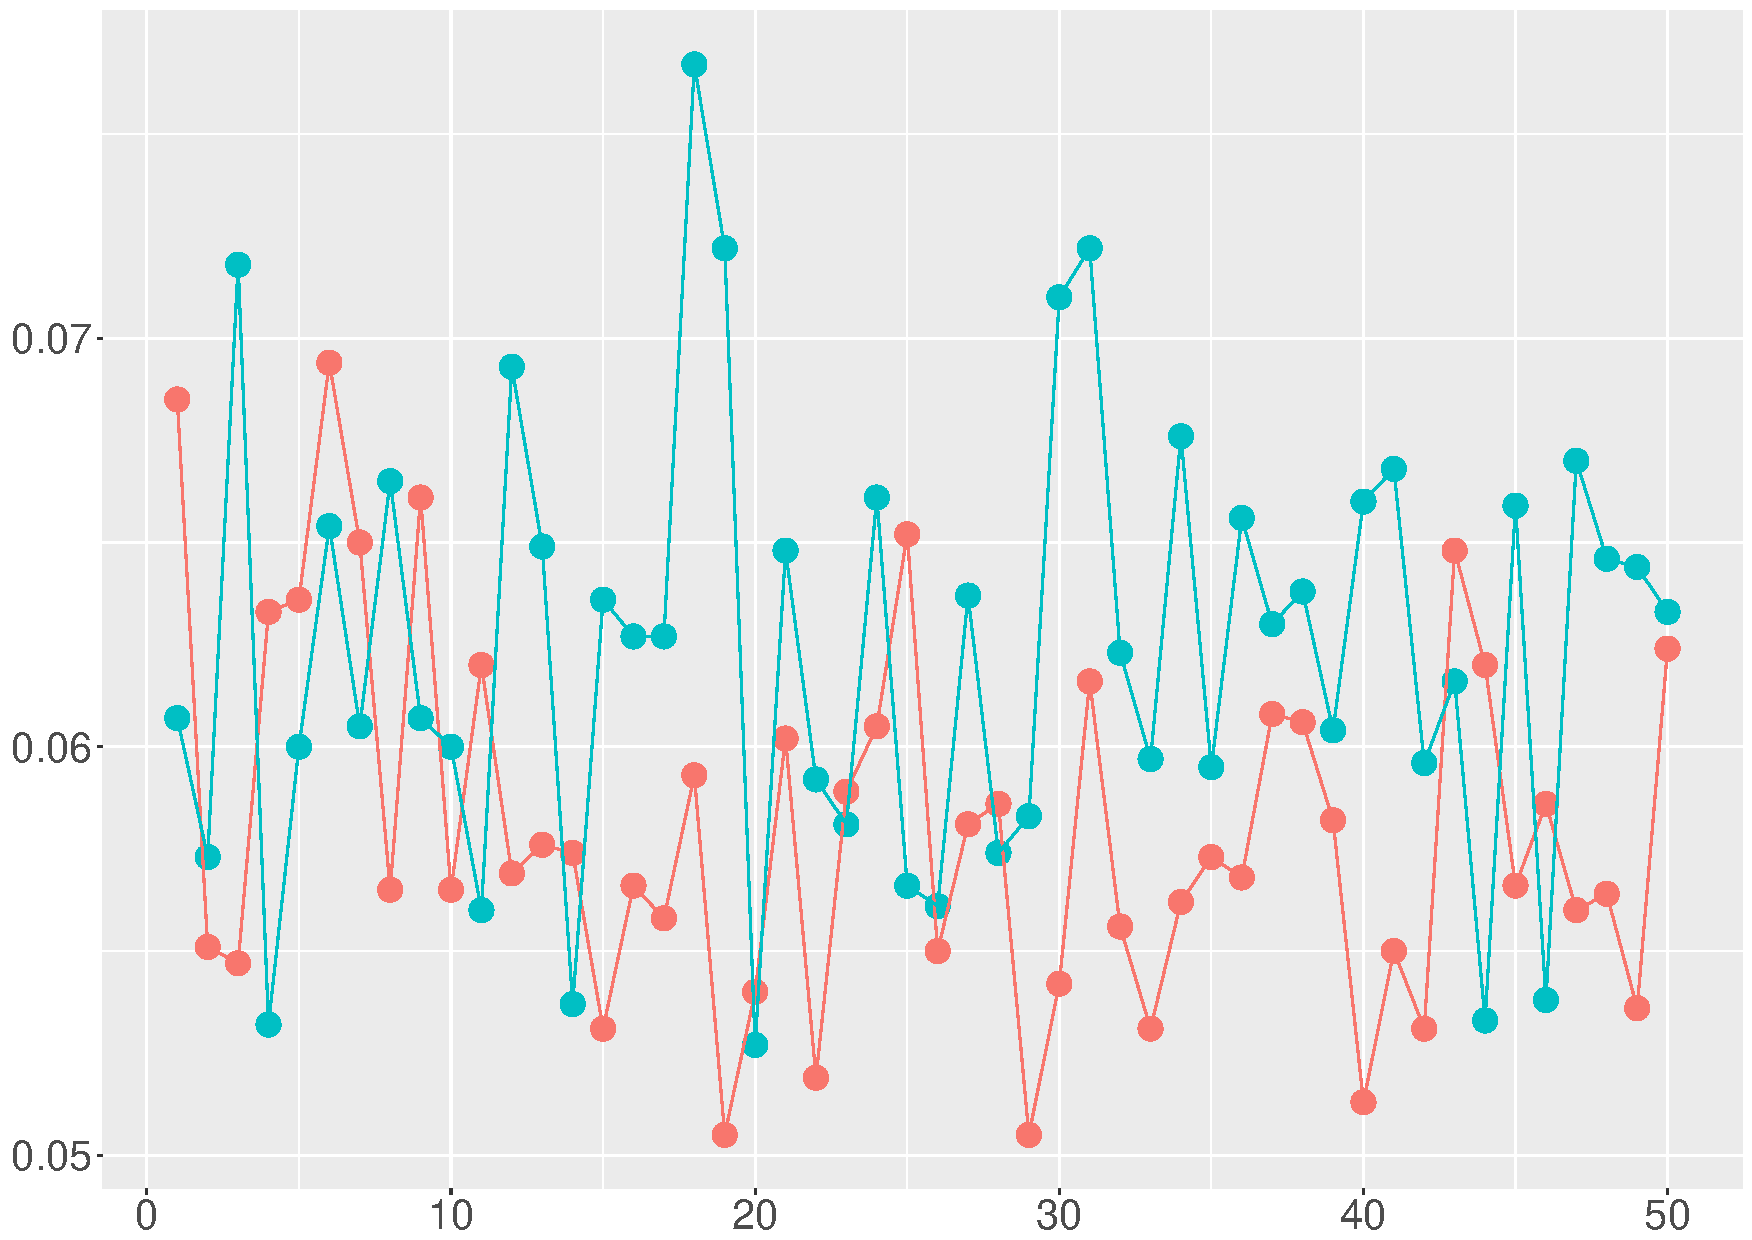
\includegraphics[width=\textwidth]{Chapters/05MCMCOU/plots/realdatacomparea1batchwindow2.pdf}
	\caption{$\alpha_1$}
\end{subfigure}
\begin{subfigure}[b]{0.45\textwidth}
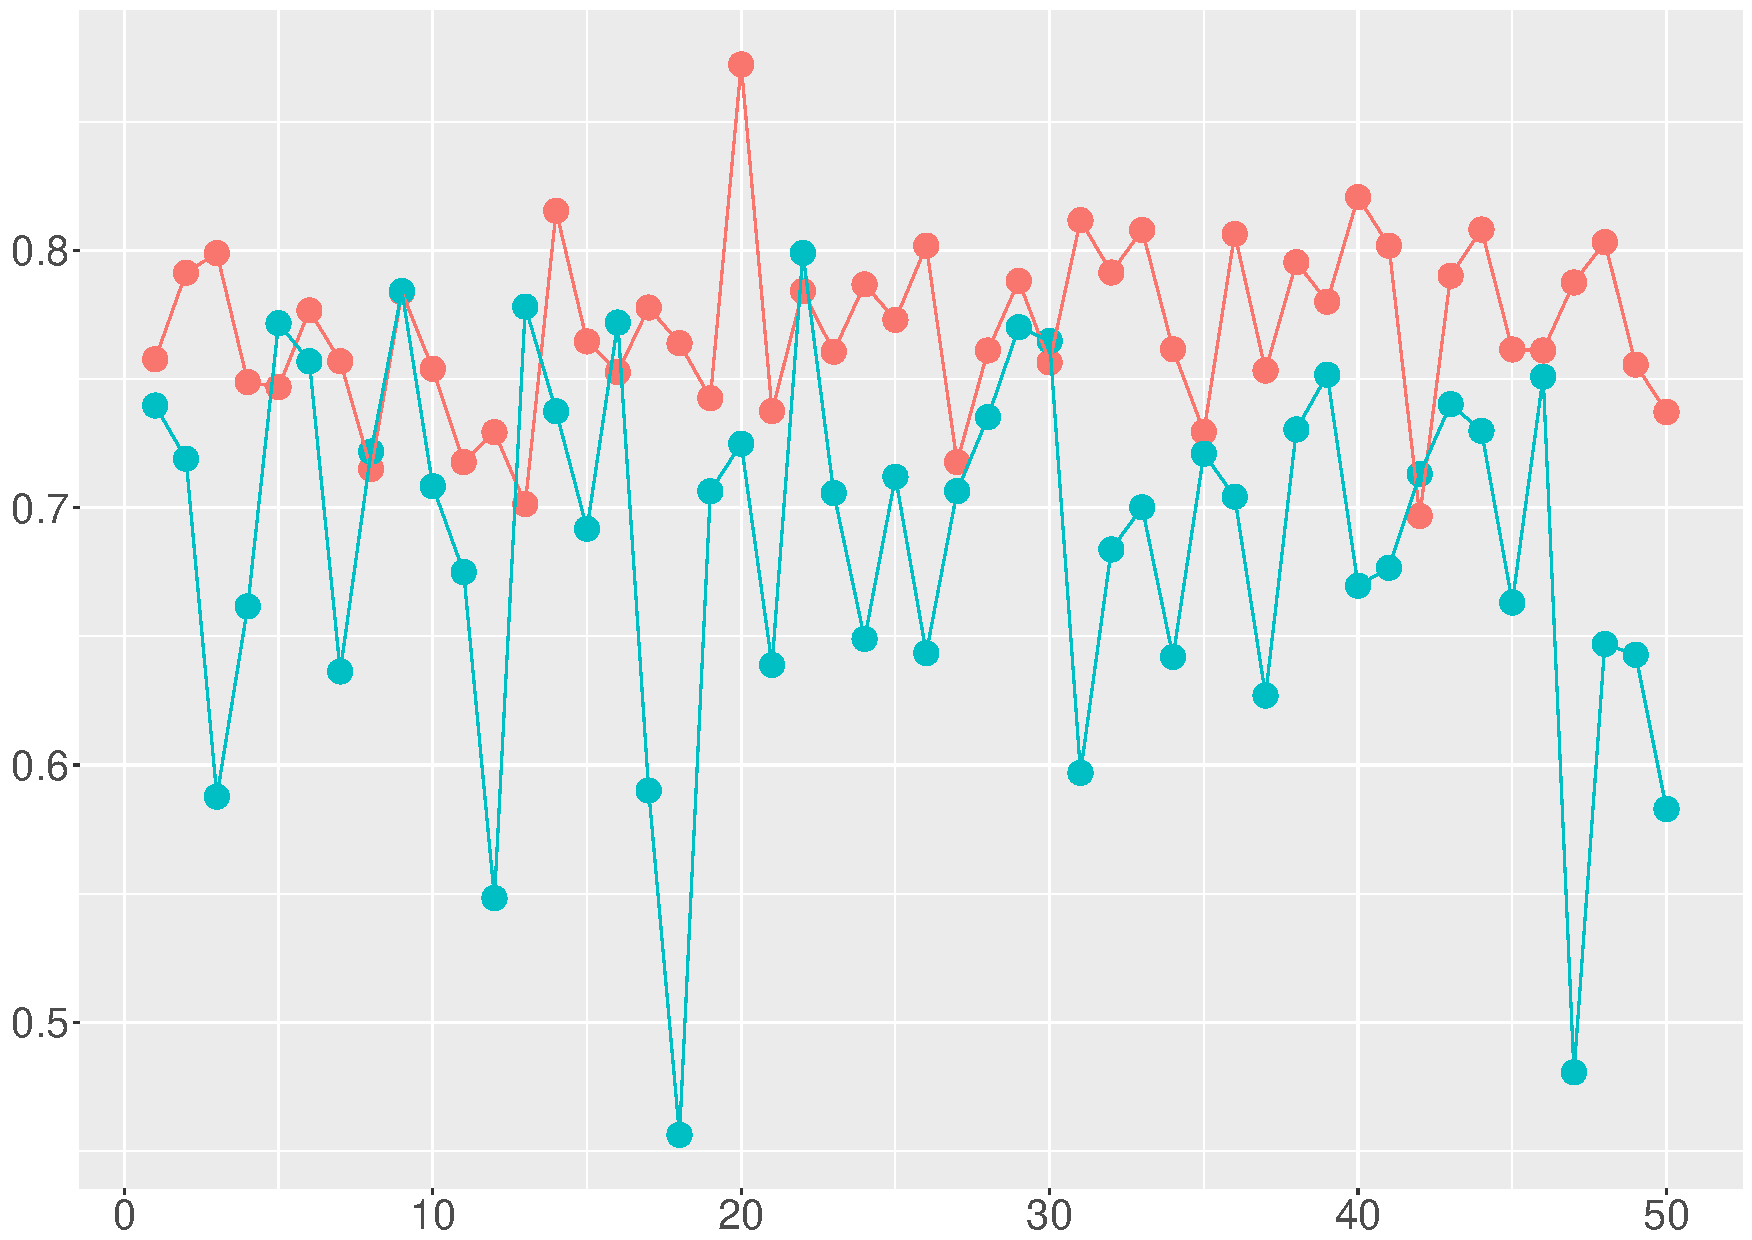
\includegraphics[width=\textwidth]{Chapters/05MCMCOU/plots/realdatacomparea2batchwindow2.pdf}
	\caption{$\alpha_2$}
\end{subfigure}
\begin{subfigure}[b]{0.45\textwidth}
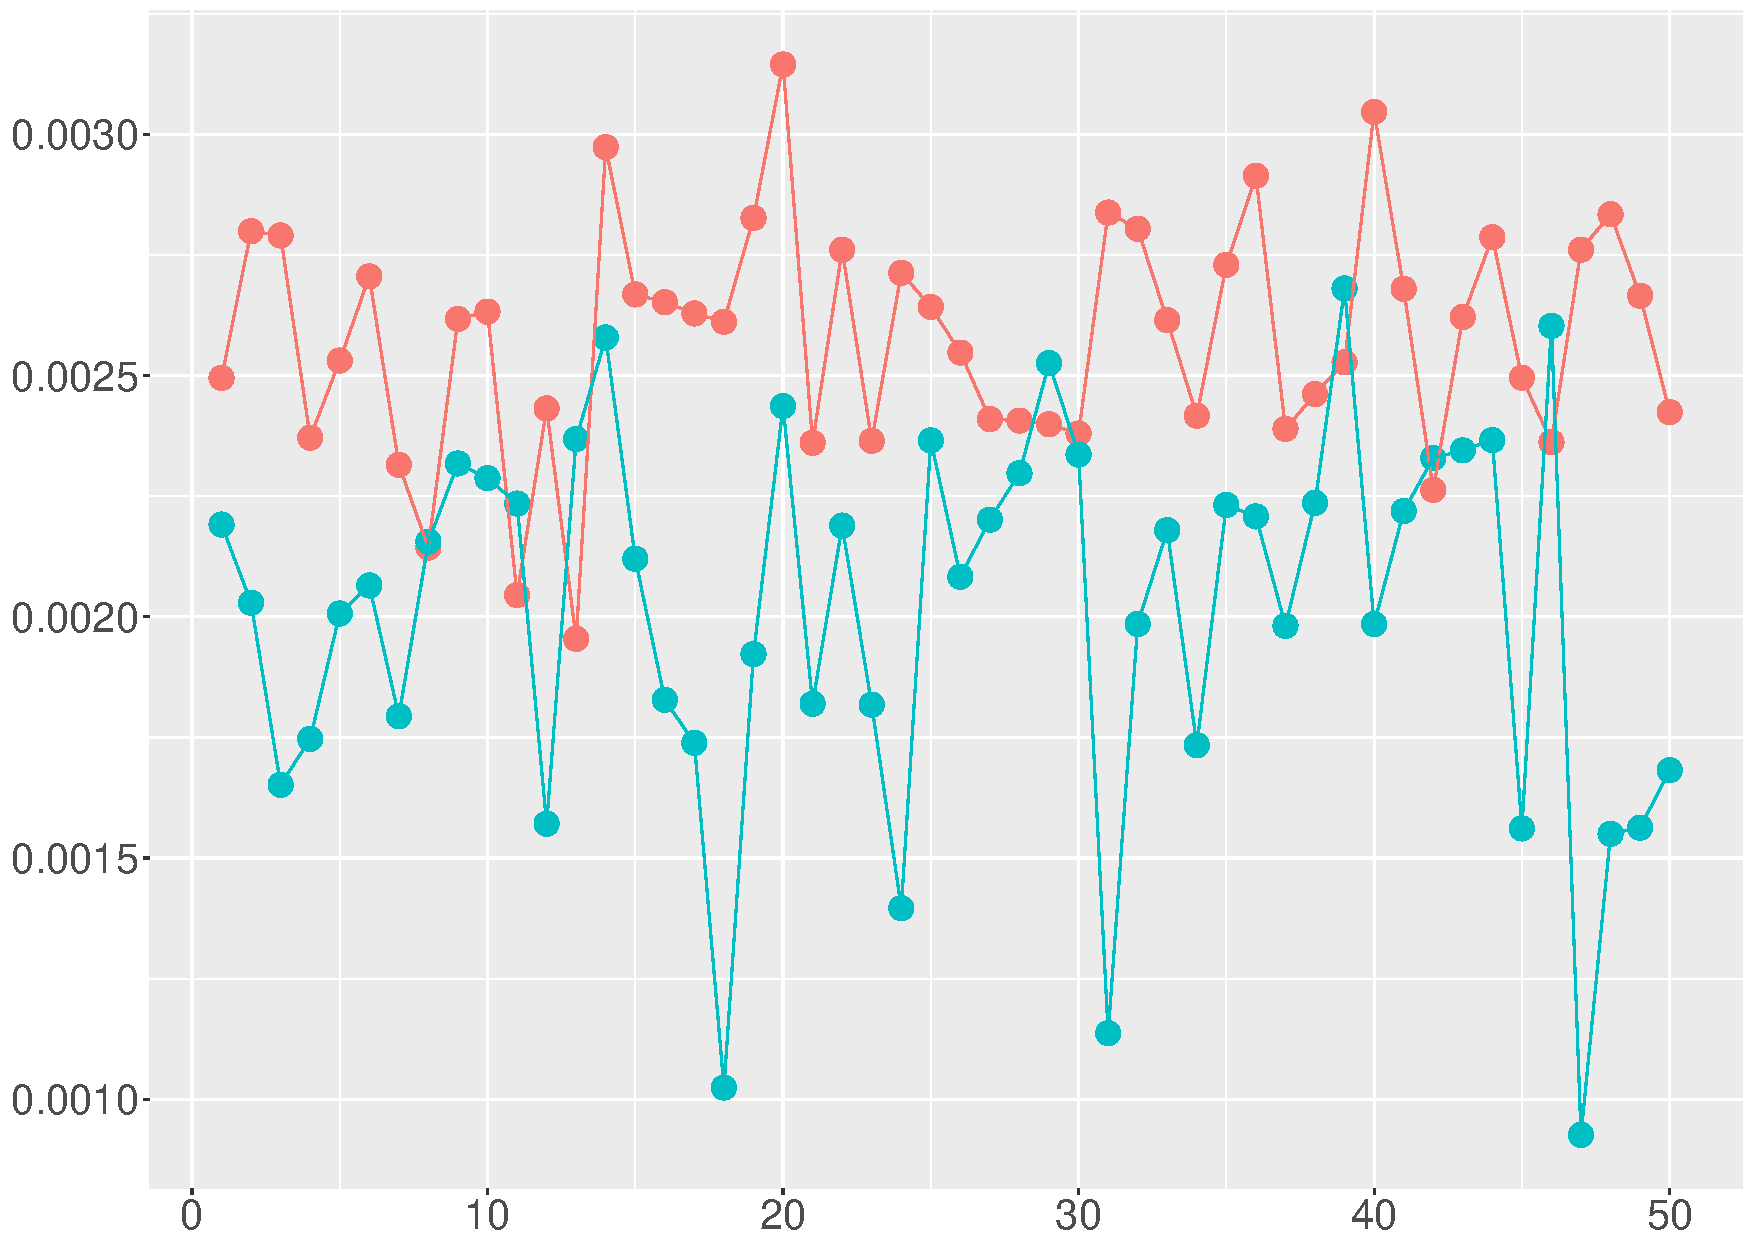
\includegraphics[width=\textwidth]{Chapters/05MCMCOU/plots/realdatacompareeffutbatchwindow2.pdf}
	\caption{EffUT}
\end{subfigure}
\begin{subfigure}[b]{0.45\textwidth}
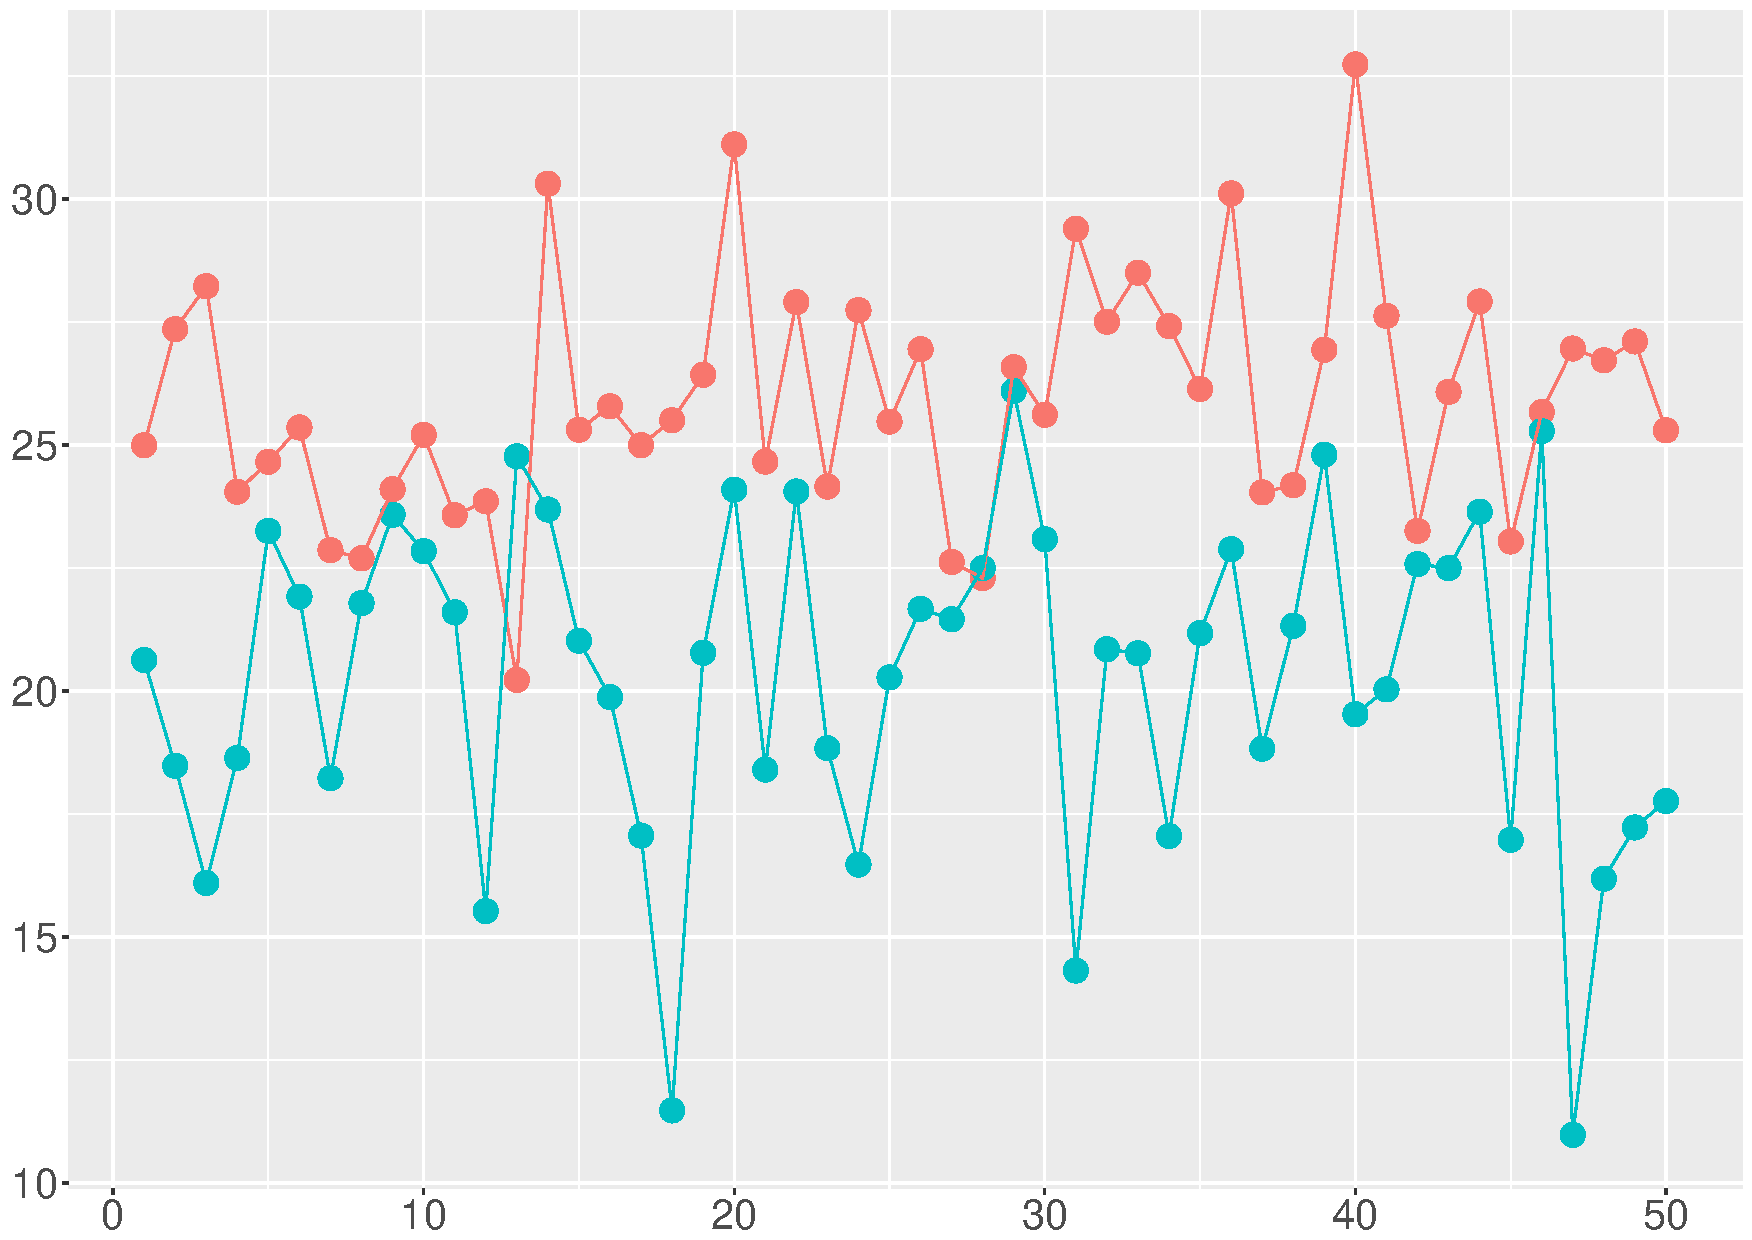
\includegraphics[width=\textwidth]{Chapters/05MCMCOU/plots/realdatacompareessutbatchwindow2.pdf}
	\caption{ESSUT}
\end{subfigure}
\caption{Comparison of $\alpha_1$, $\alpha_2$, EffUT and ESSUT between batch MCMC (orange) and sliding window MCMC (green). }\label{batchwindowkeyfeature}
\end{figure}

\begin{figure}[h]
\centering
\begin{subfigure}[b]{0.45\textwidth}
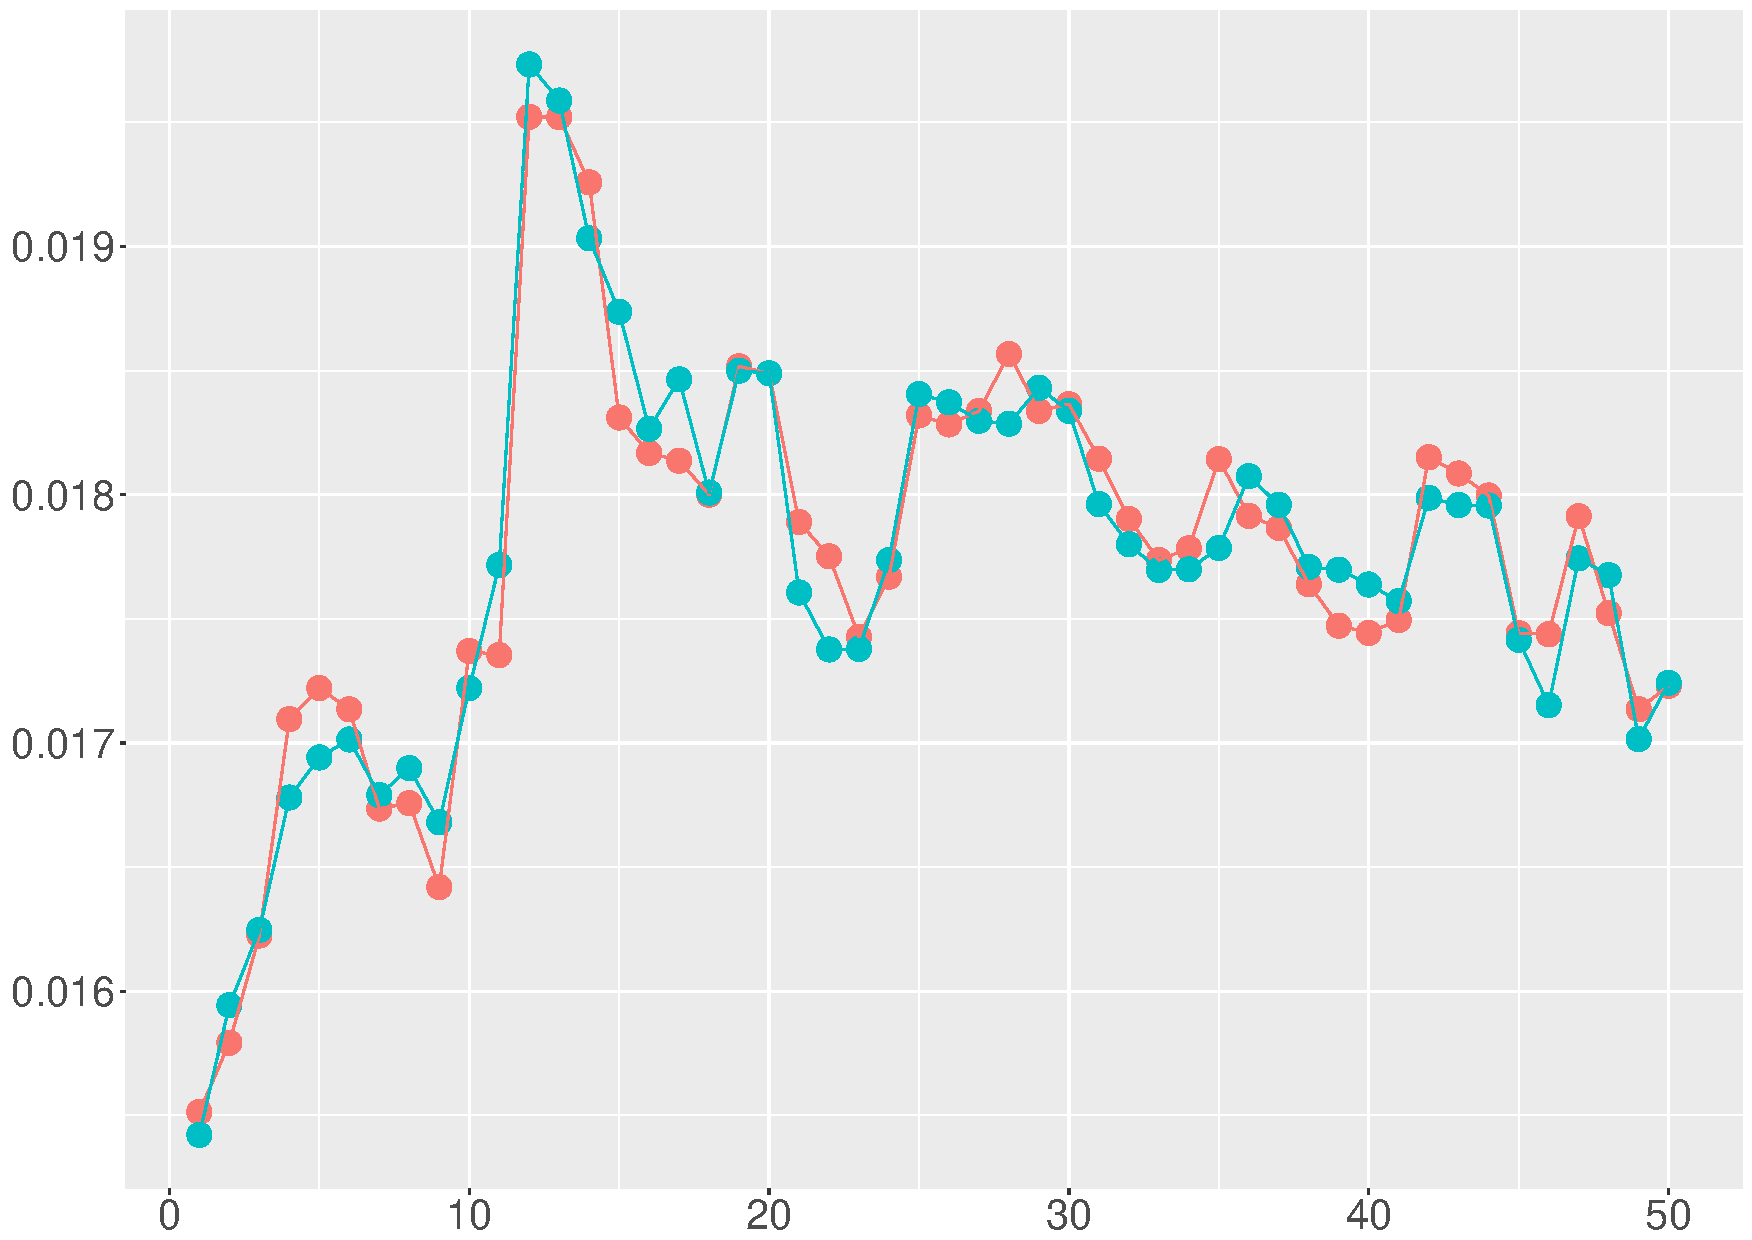
\includegraphics[width=\textwidth]{Chapters/05MCMCOU/plots/realdatacomparegambatchwindow2.pdf}
	\caption{$\gamma$}
\end{subfigure}
\begin{subfigure}[b]{0.45\textwidth}
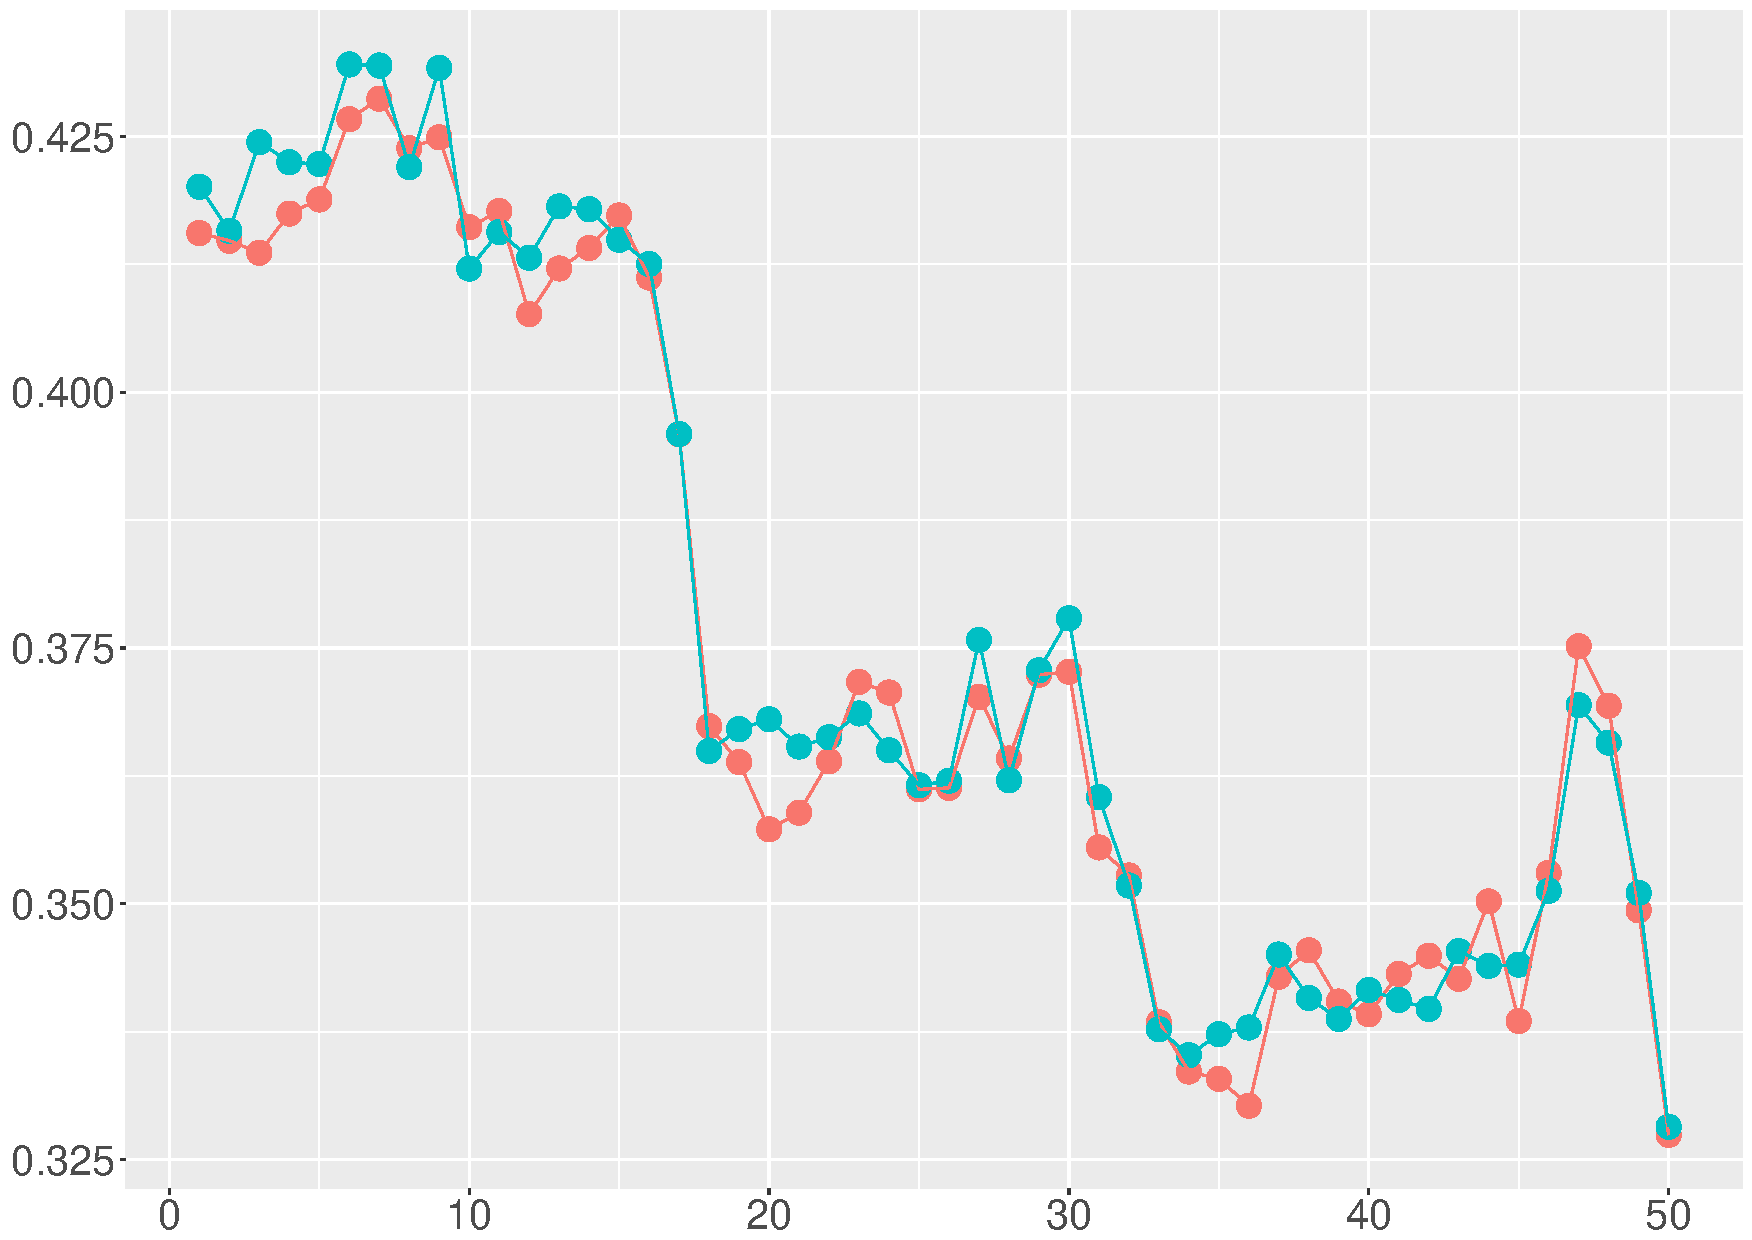
\includegraphics[width=\textwidth]{Chapters/05MCMCOU/plots/realdatacomparexi2batchwindow2.pdf}
	\caption{$\xi^2$}
\end{subfigure}
\begin{subfigure}[b]{0.45\textwidth}
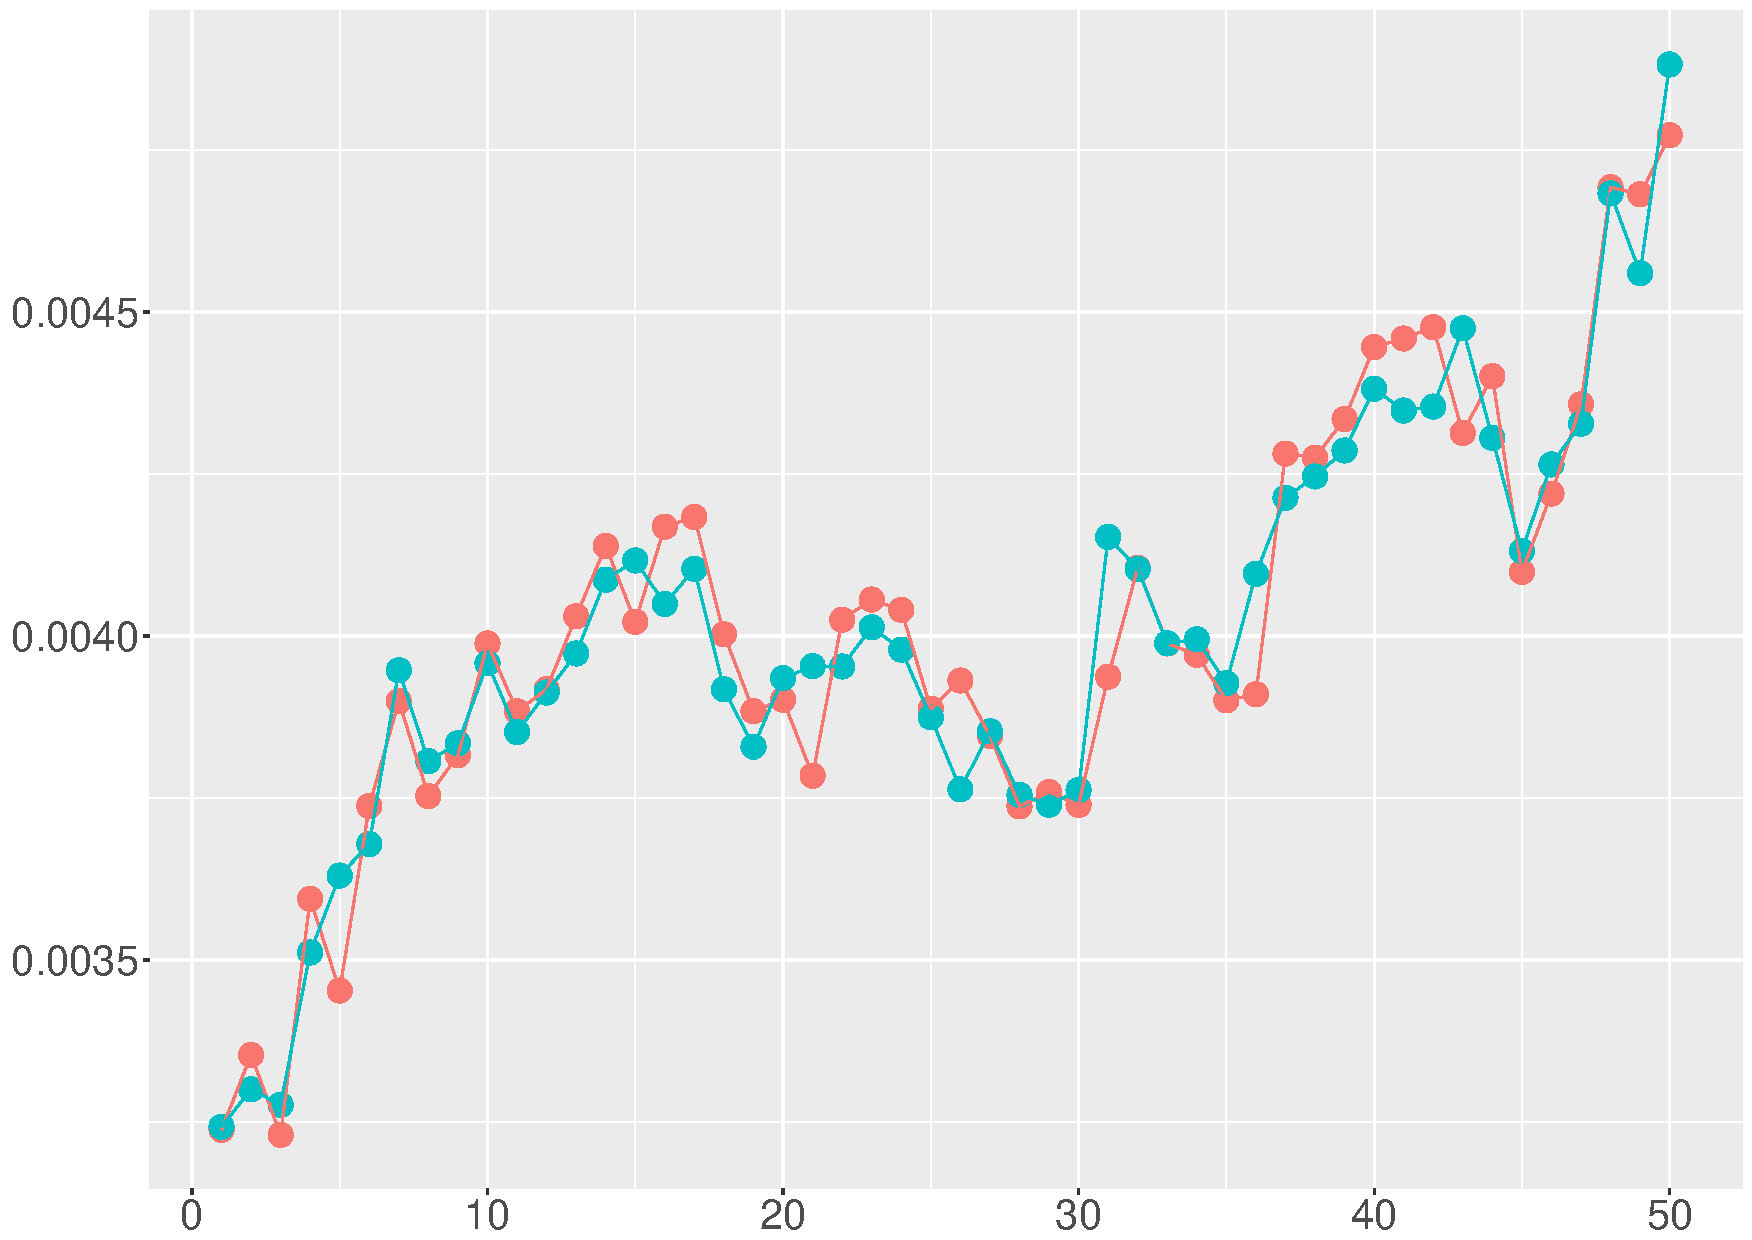
\includegraphics[width=\textwidth]{Chapters/05MCMCOU/plots/realdatacomparelab2batchwindow2.pdf}
\caption{$\lambda^2$}
\end{subfigure}
\begin{subfigure}[b]{0.45\textwidth}
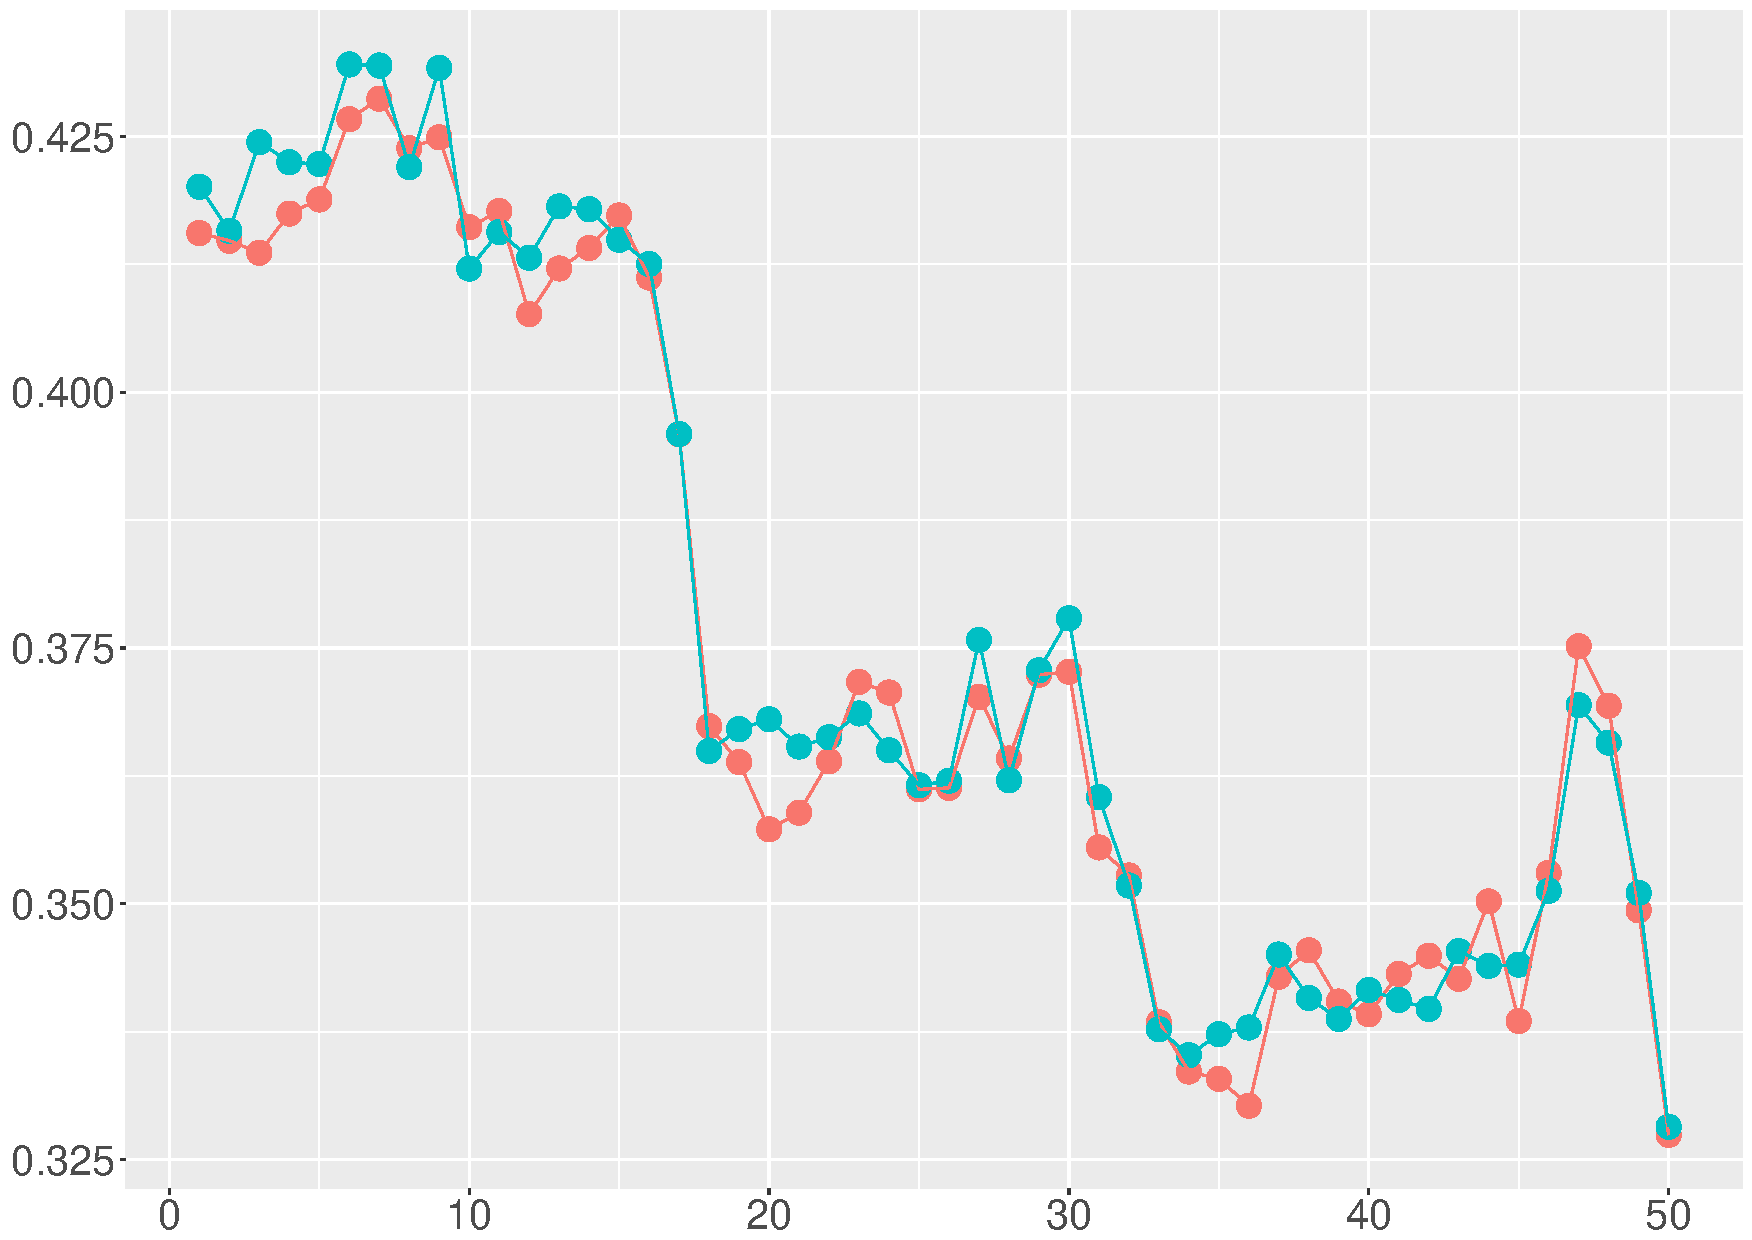
\includegraphics[width=\textwidth]{Chapters/05MCMCOU/plots/realdatacomparesig2batchwindow2.pdf}
\caption{$\sigma^2$}
\end{subfigure}
\begin{subfigure}[b]{0.45\textwidth}
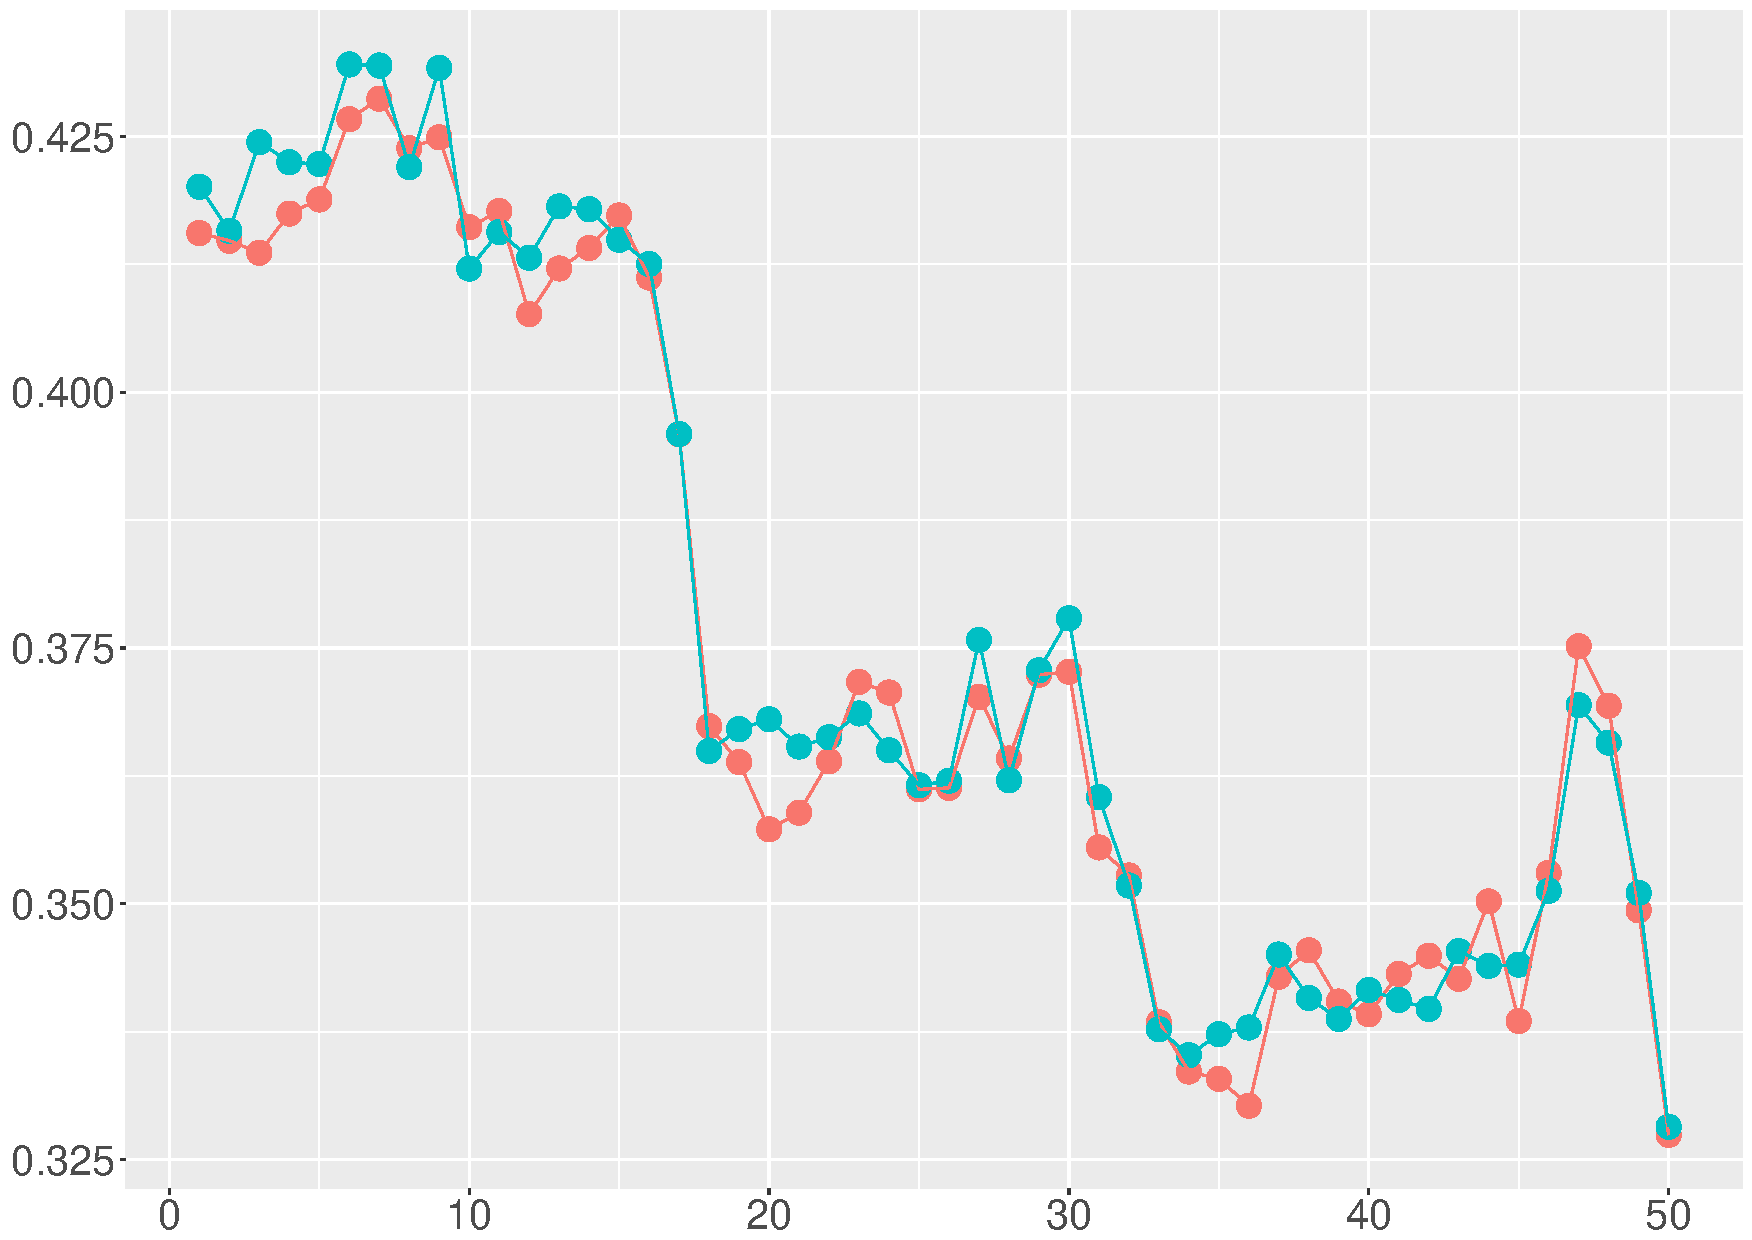
\includegraphics[width=\textwidth]{Chapters/05MCMCOU/plots/realdatacomparetau2batchwindow2.pdf}
\caption{$\tau^2$}
\end{subfigure}
\caption{Comparison of parameters estimation between batch MCMC (orange) and sliding window MCMC (green). }\label{batchwindowparameter}
\end{figure}



\clearpage

\section{Parameter Evolution Visualization}

\begin{figure}[h]
\centering
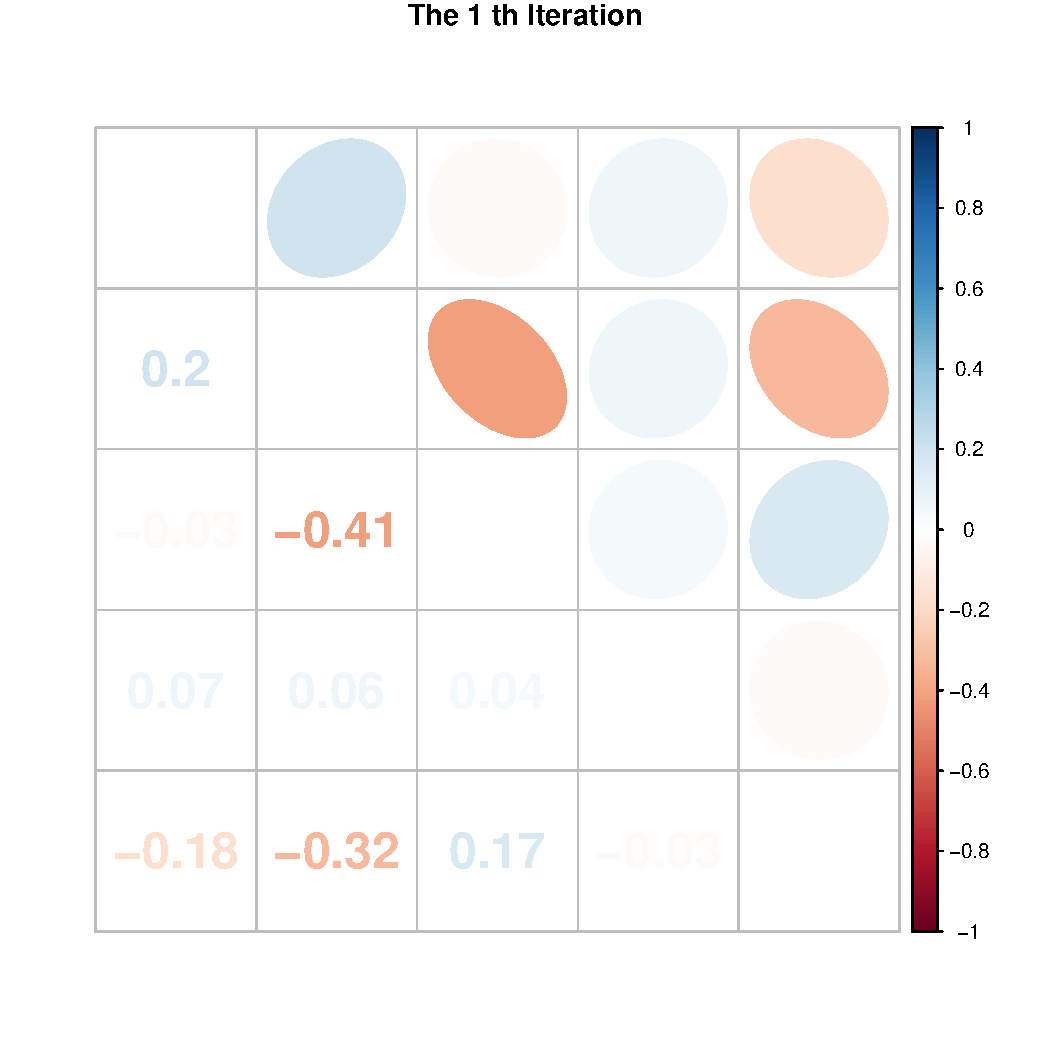
\includegraphics[width=0.3\textwidth,height=0.18\textheight]{Chapters/05MCMCOU/plots/paraEvolution/corMatrix1.pdf}
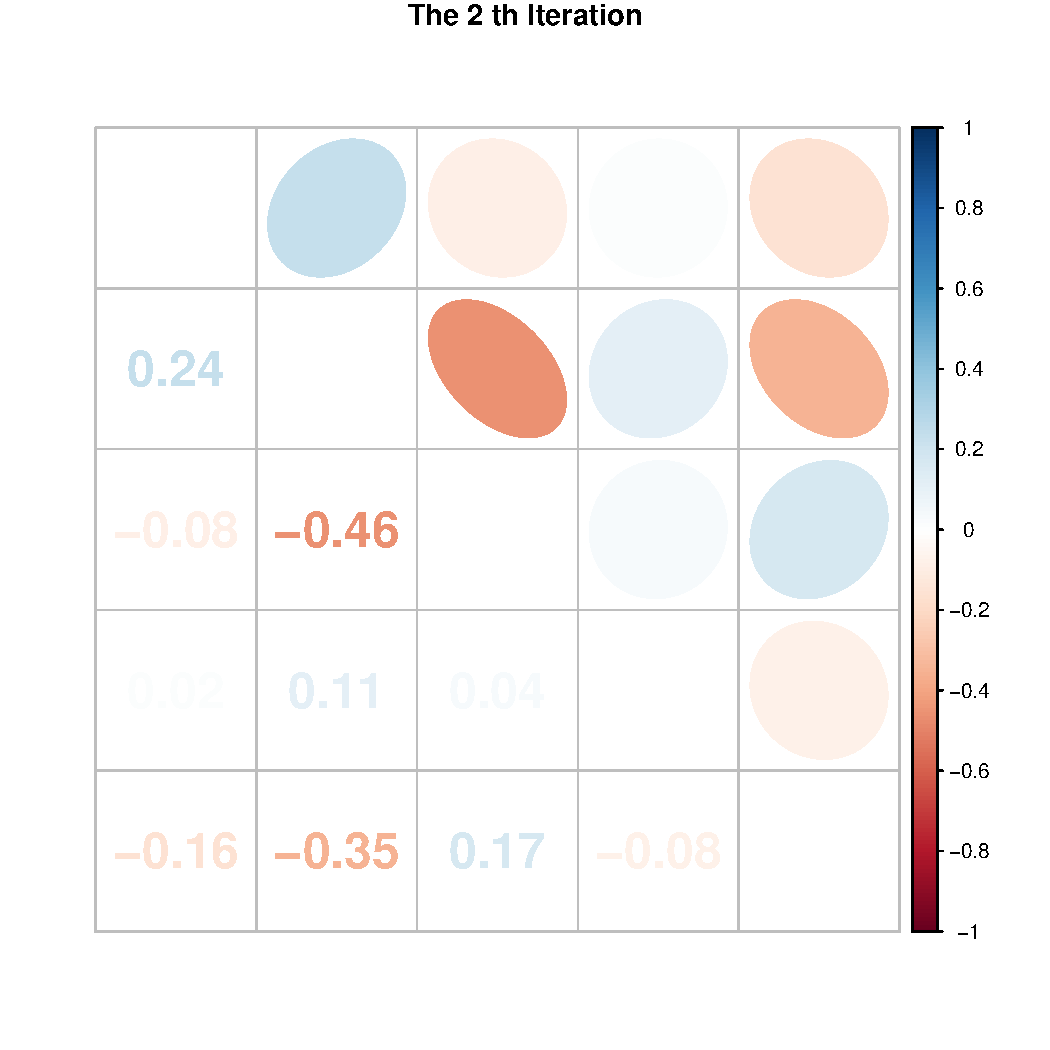
\includegraphics[width=0.3\textwidth,height=0.18\textheight]{Chapters/05MCMCOU/plots/paraEvolution/corMatrix2.pdf}
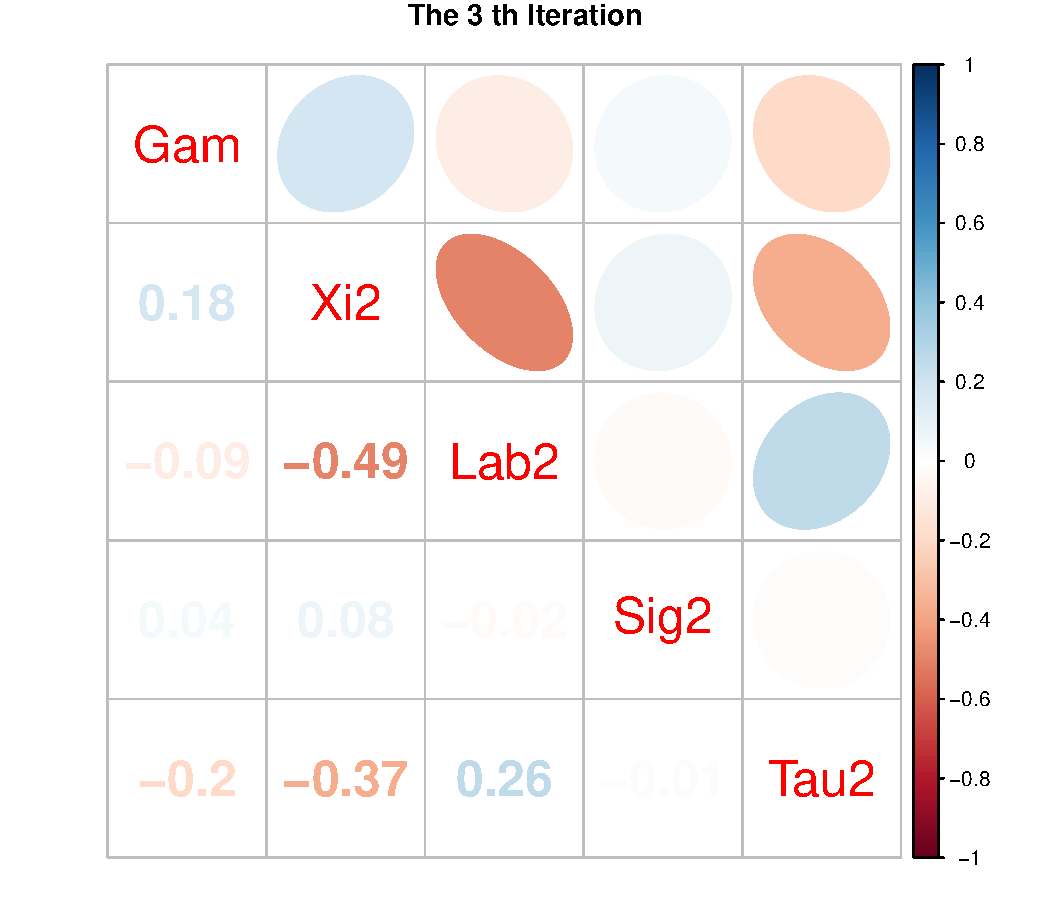
\includegraphics[width=0.3\textwidth,height=0.18\textheight]{Chapters/05MCMCOU/plots/paraEvolution/corMatrix3.pdf}
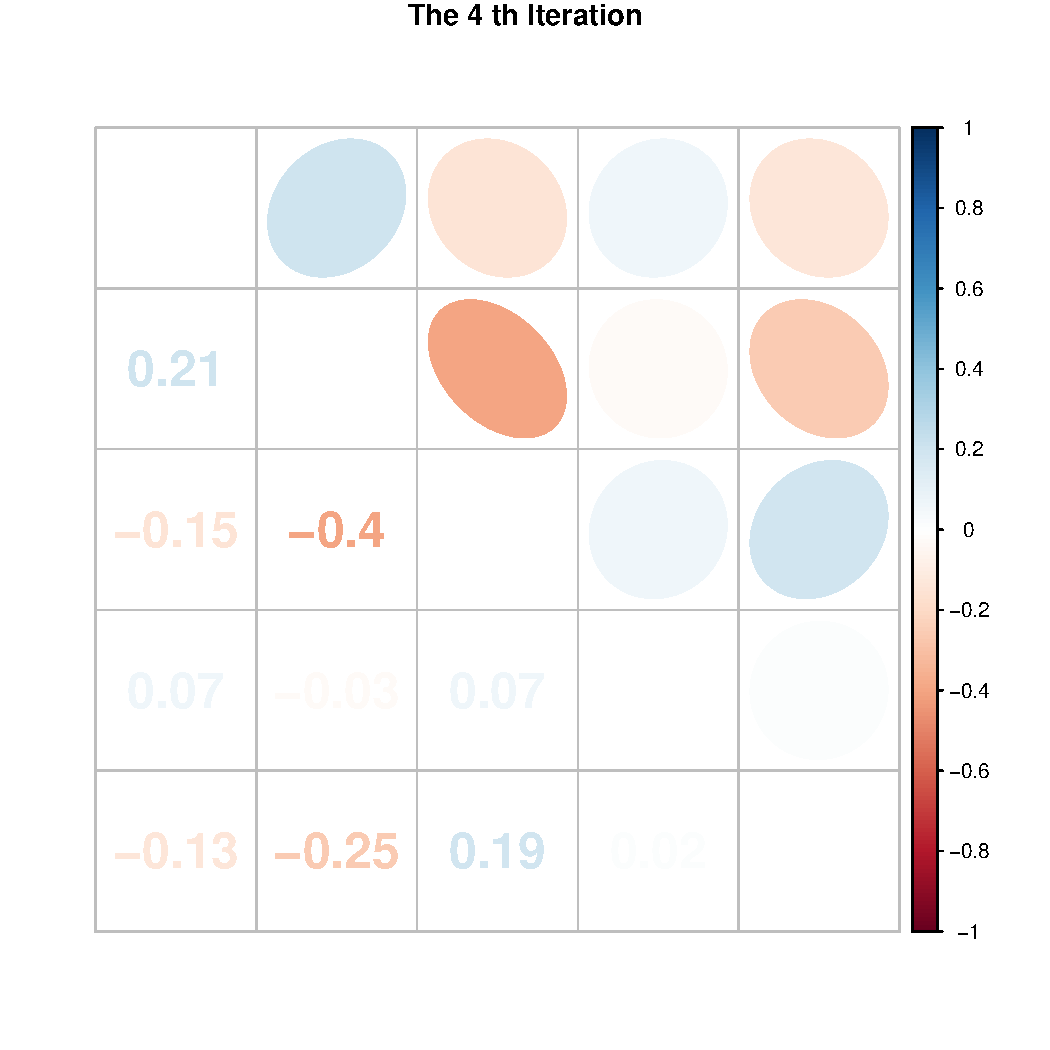
\includegraphics[width=0.3\textwidth,height=0.18\textheight]{Chapters/05MCMCOU/plots/paraEvolution/corMatrix4.pdf}
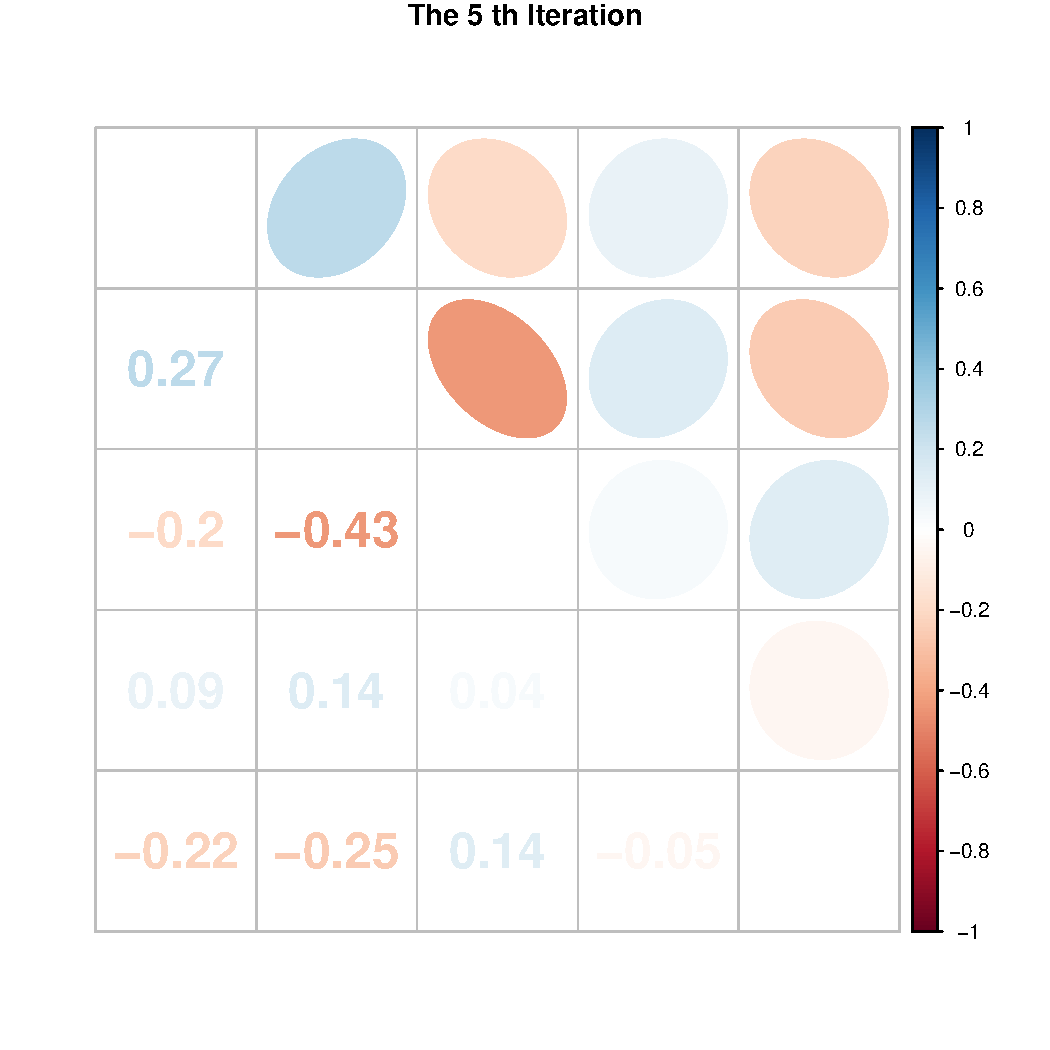
\includegraphics[width=0.3\textwidth,height=0.18\textheight]{Chapters/05MCMCOU/plots/paraEvolution/corMatrix5.pdf}
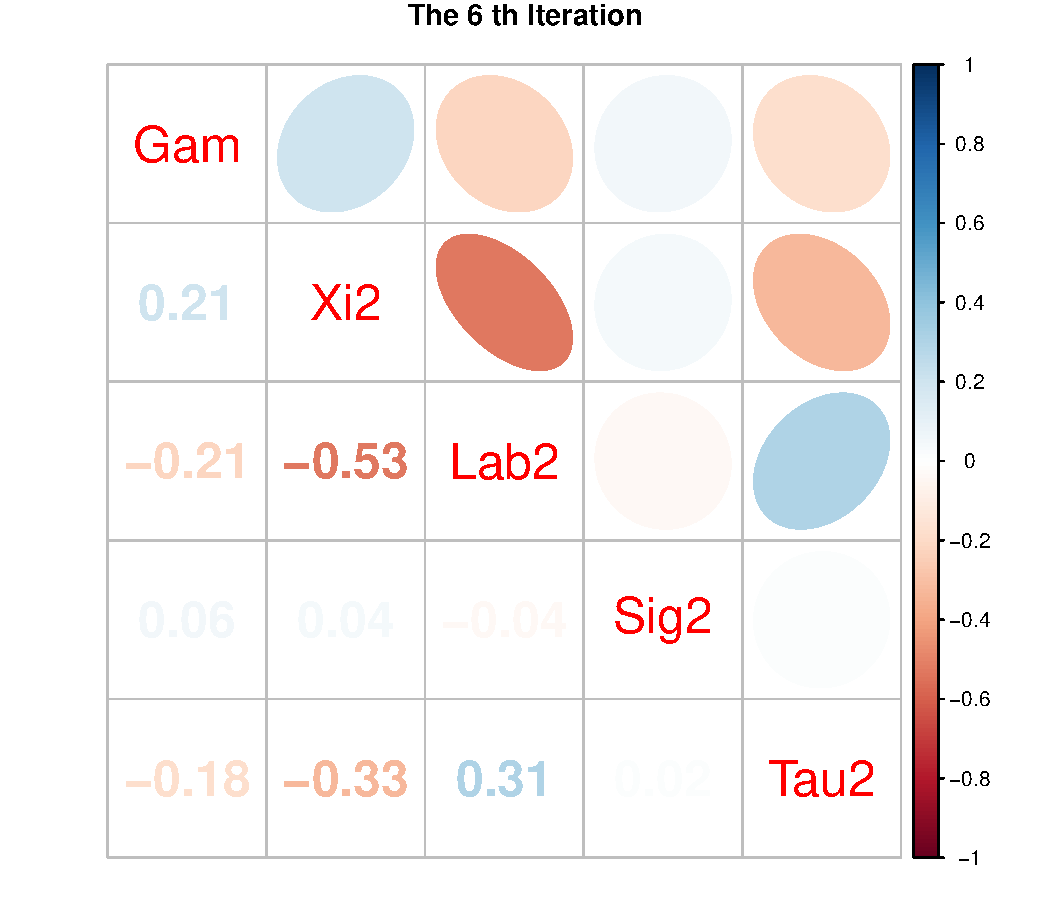
\includegraphics[width=0.3\textwidth,height=0.18\textheight]{Chapters/05MCMCOU/plots/paraEvolution/corMatrix6.pdf}
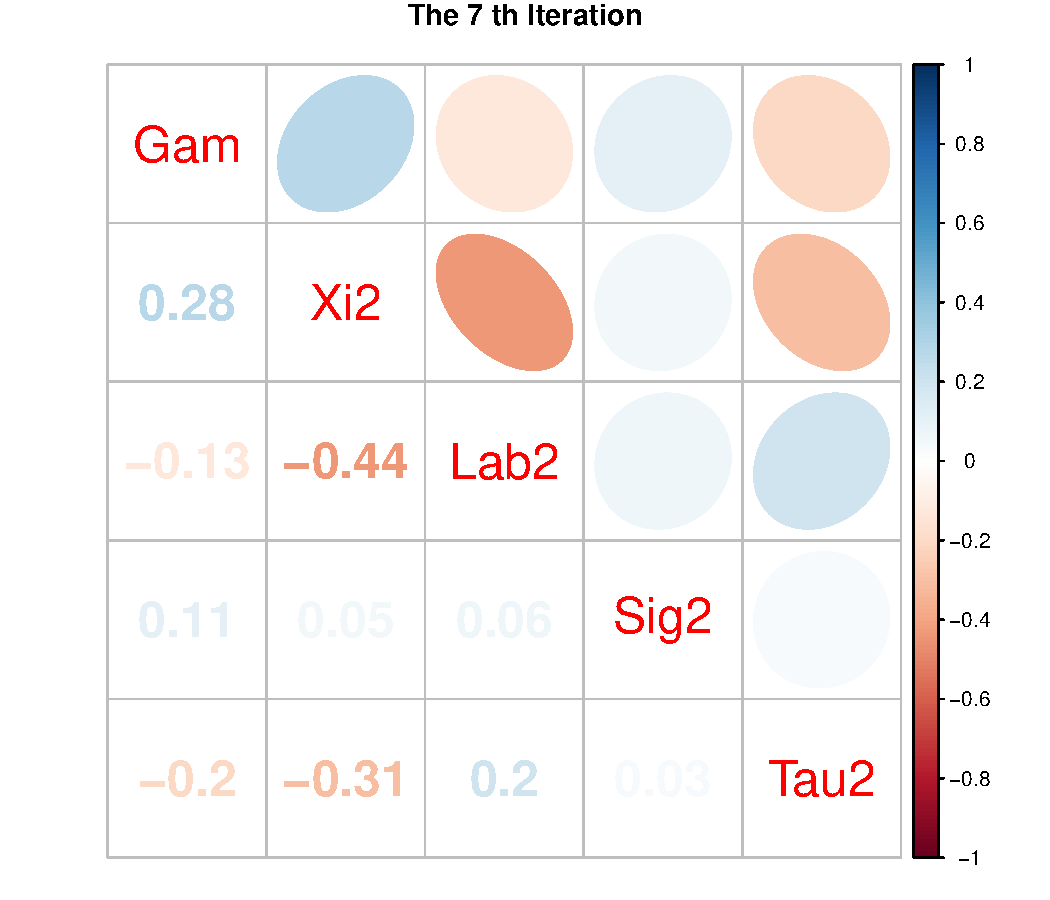
\includegraphics[width=0.3\textwidth,height=0.18\textheight]{Chapters/05MCMCOU/plots/paraEvolution/corMatrix7.pdf}
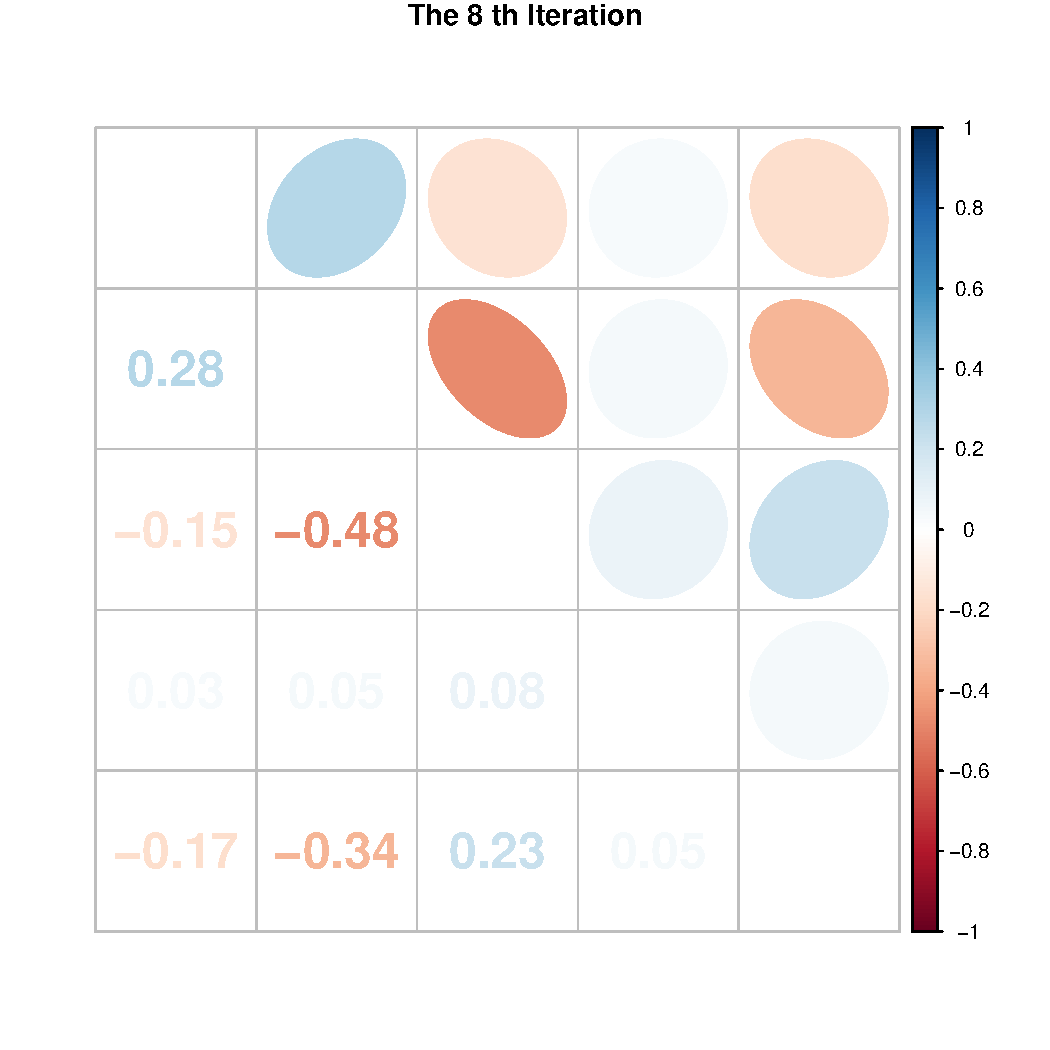
\includegraphics[width=0.3\textwidth,height=0.18\textheight]{Chapters/05MCMCOU/plots/paraEvolution/corMatrix8.pdf}
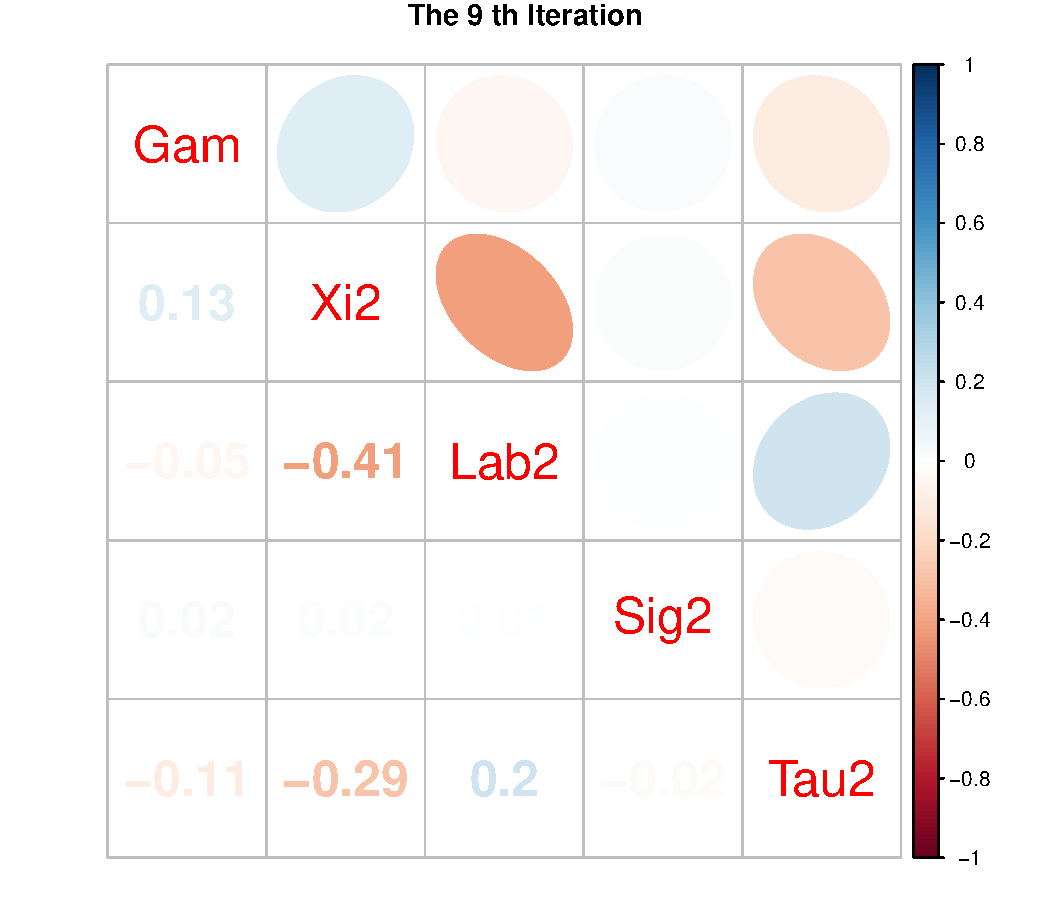
\includegraphics[width=0.3\textwidth,height=0.18\textheight]{Chapters/05MCMCOU/plots/paraEvolution/corMatrix9.pdf}
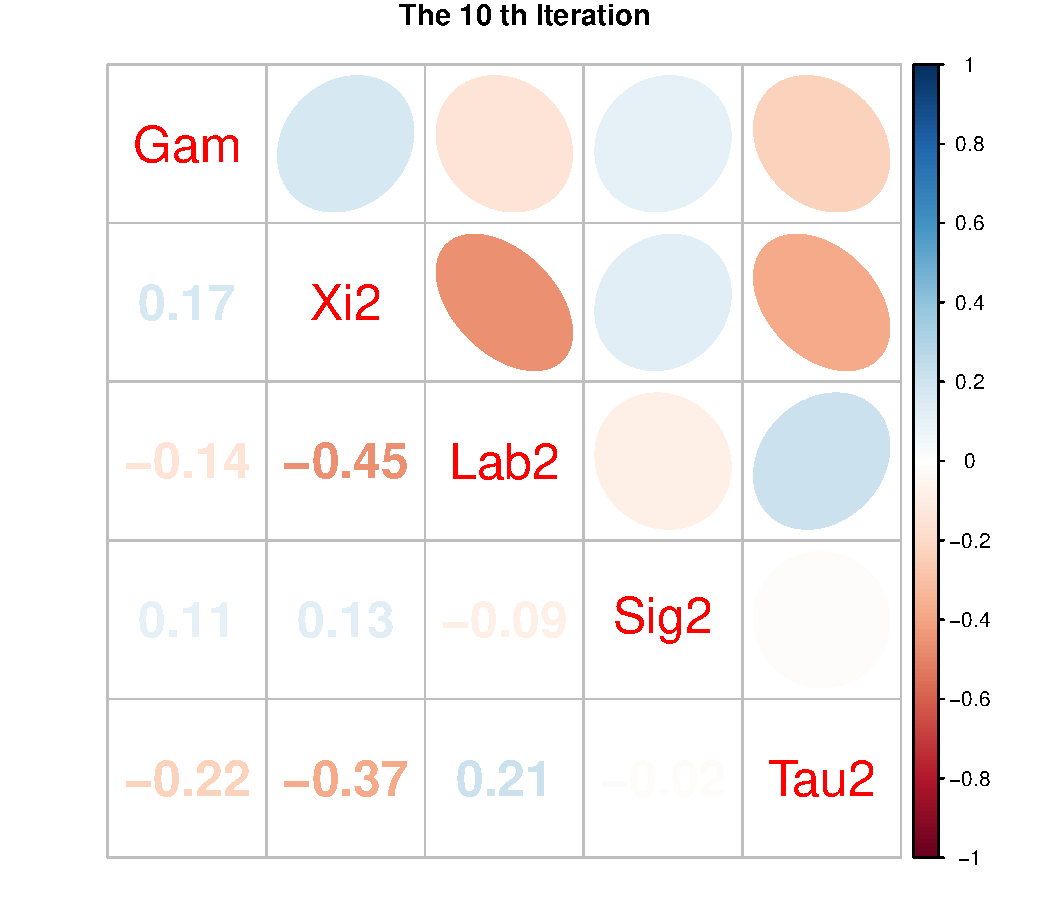
\includegraphics[width=0.3\textwidth,height=0.18\textheight]{Chapters/05MCMCOU/plots/paraEvolution/corMatrix10.pdf}
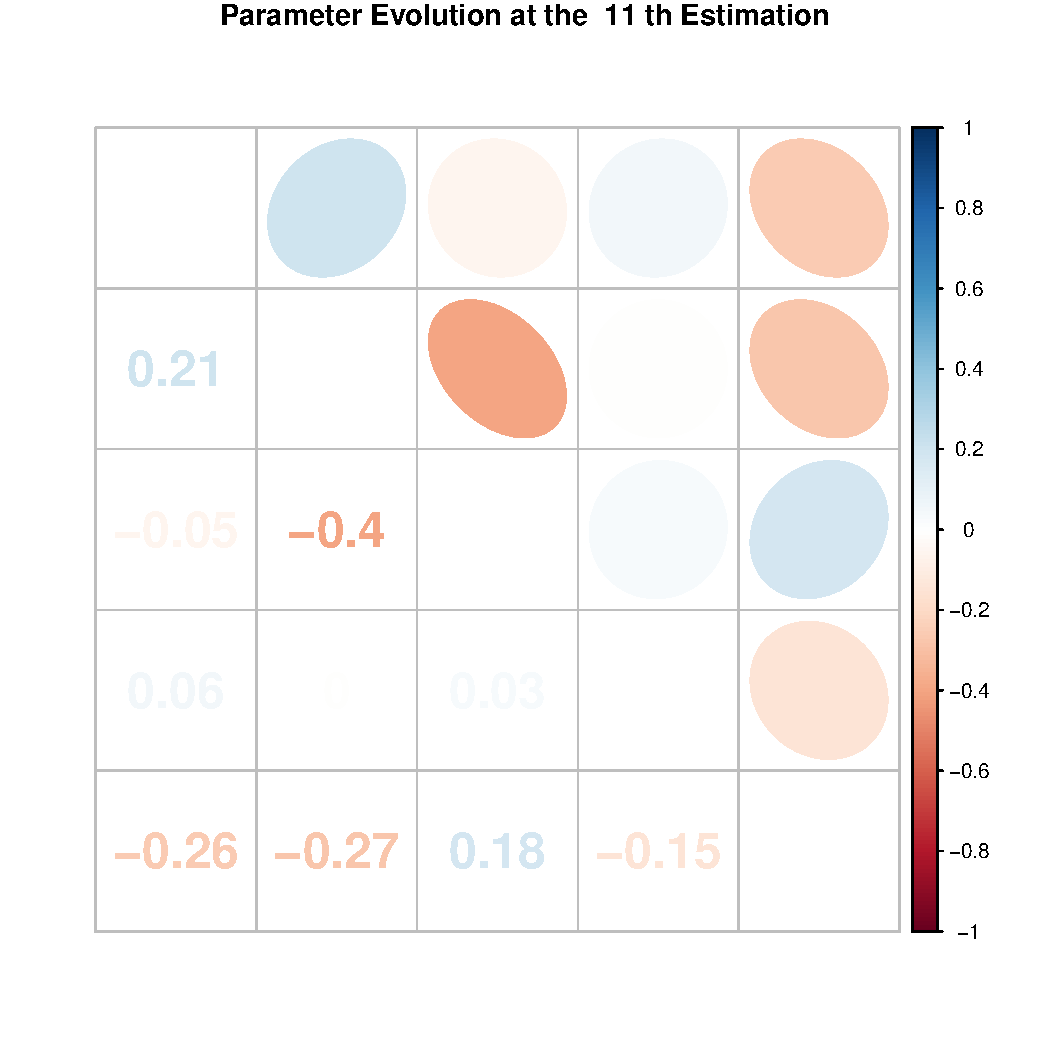
\includegraphics[width=0.3\textwidth,height=0.18\textheight]{Chapters/05MCMCOU/plots/paraEvolution/corMatrix11.pdf}
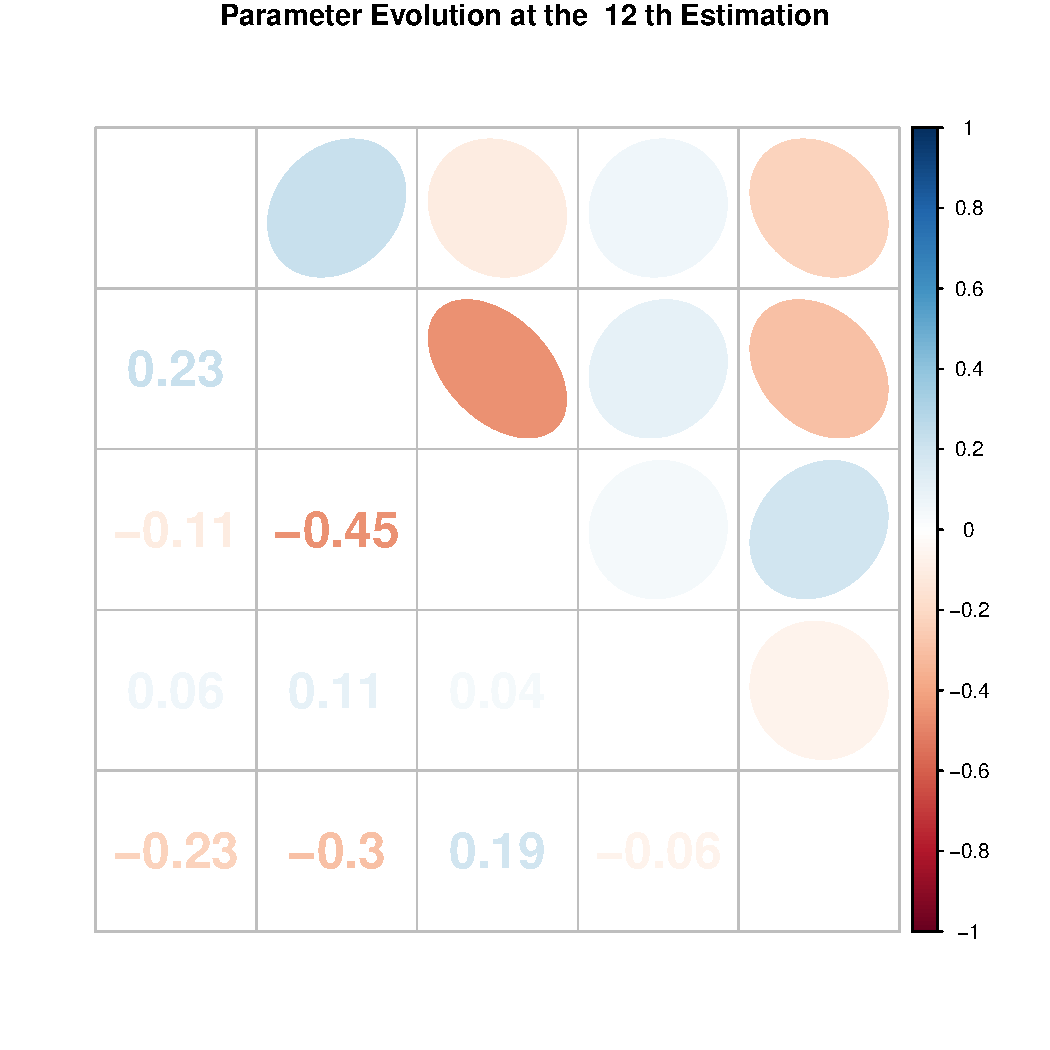
\includegraphics[width=0.3\textwidth,height=0.18\textheight]{Chapters/05MCMCOU/plots/paraEvolution/corMatrix12.pdf}
%\caption{Parameter Evolution Visualization. }
\end{figure}
\begin{figure}[h]\ContinuedFloat
\centering
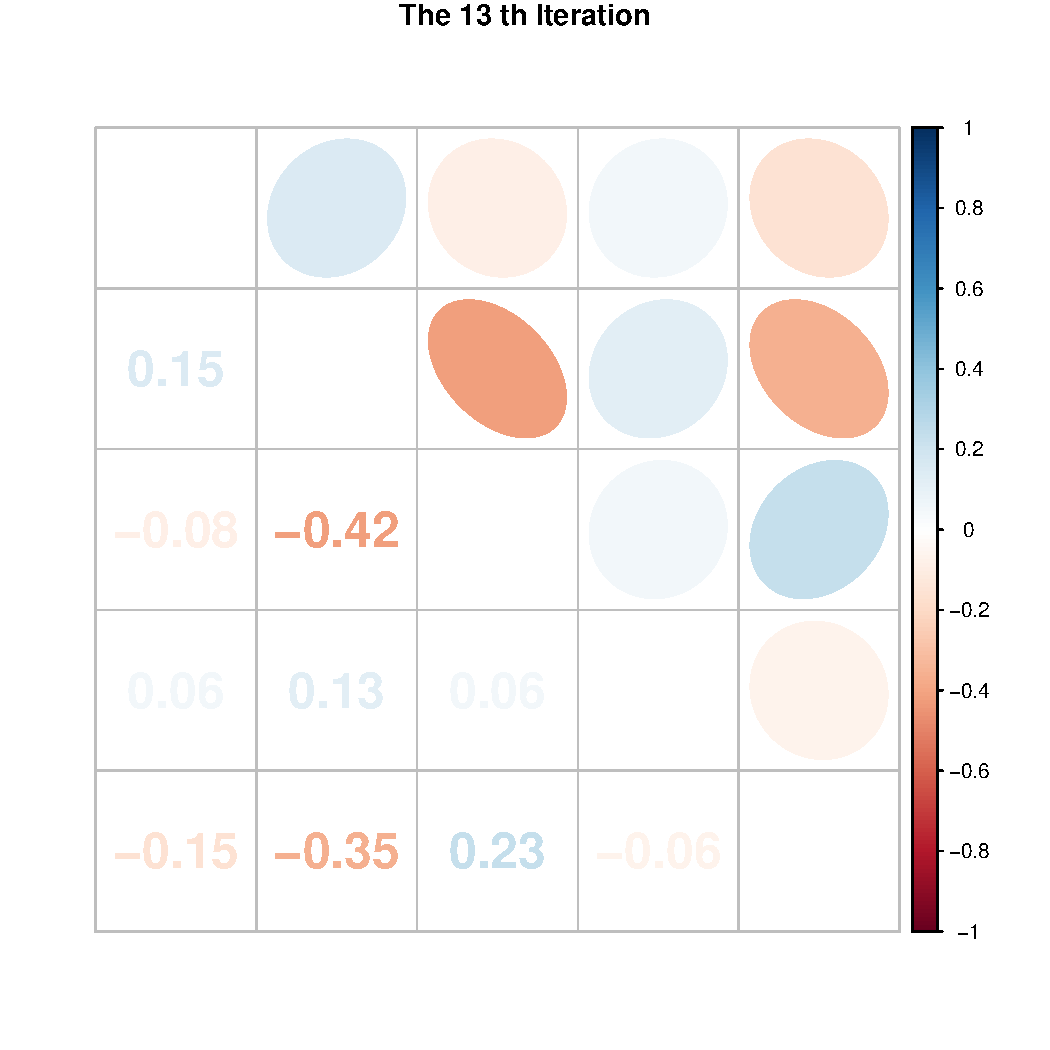
\includegraphics[width=0.3\textwidth,height=0.2\textheight]{Chapters/05MCMCOU/plots/paraEvolution/corMatrix13.pdf}
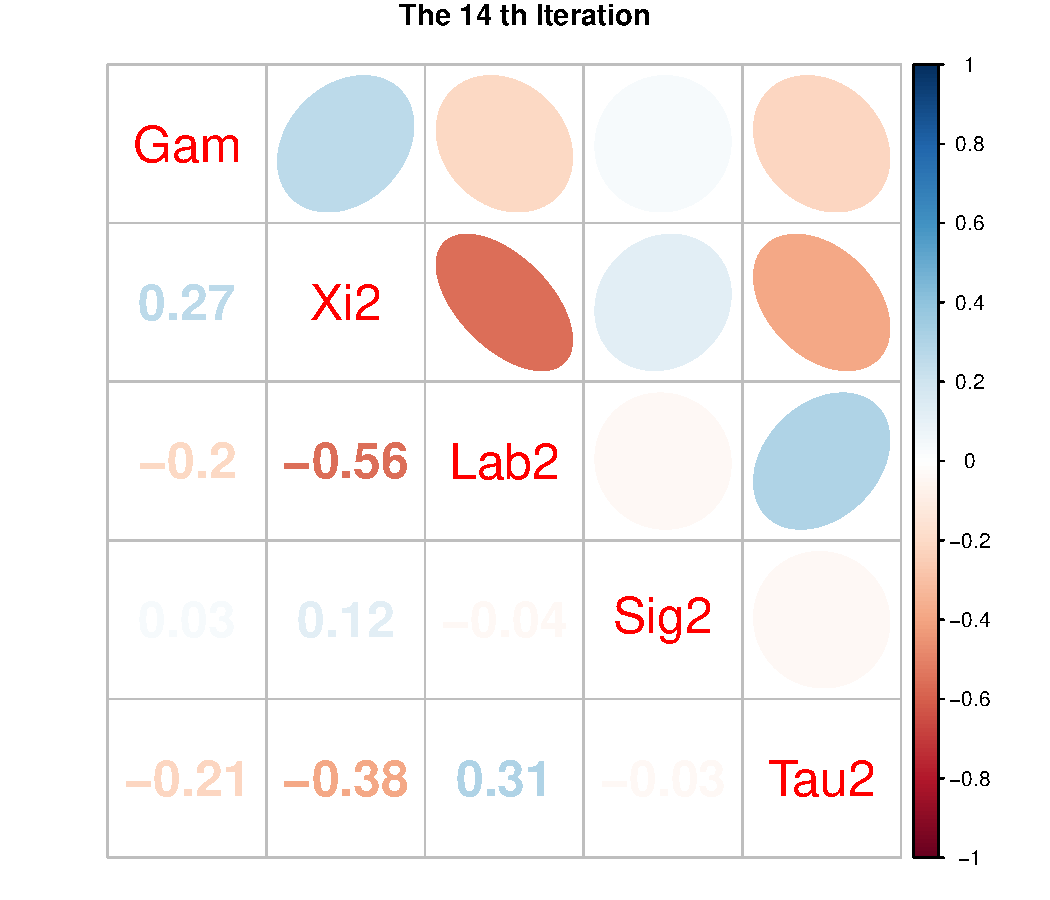
\includegraphics[width=0.3\textwidth,height=0.2\textheight]{Chapters/05MCMCOU/plots/paraEvolution/corMatrix14.pdf}
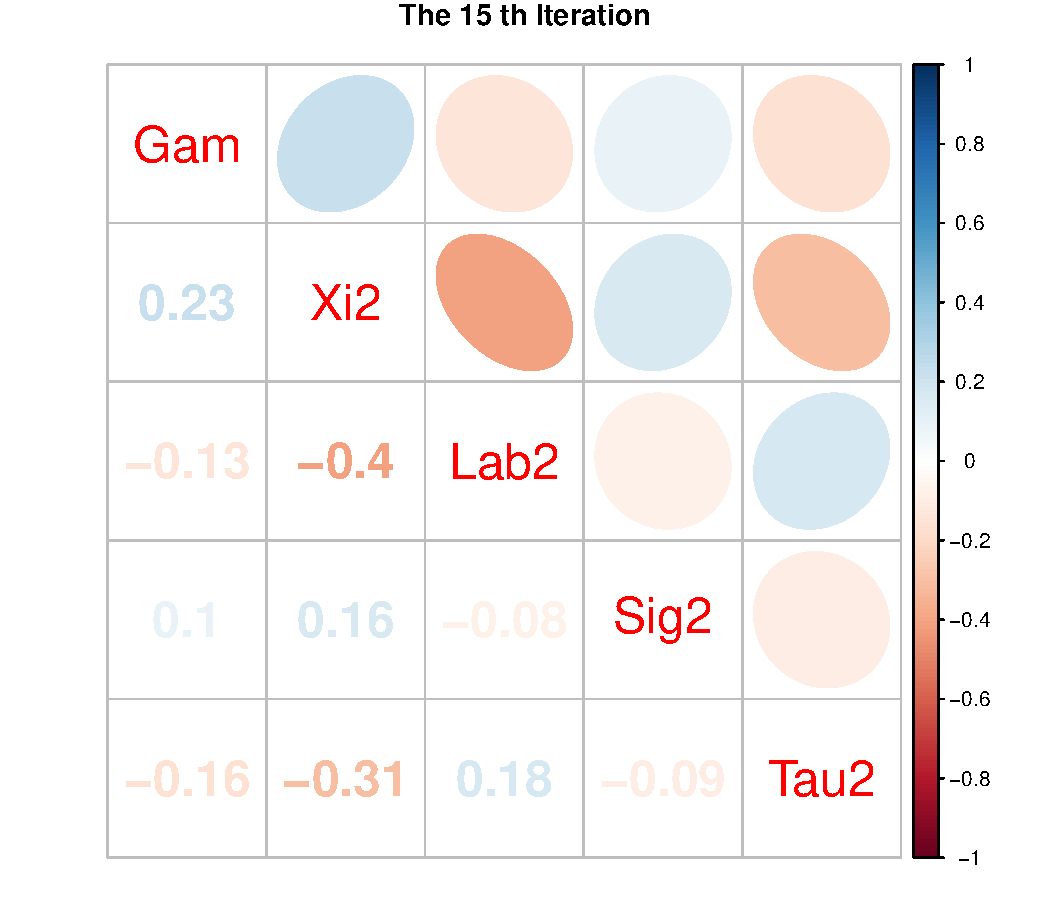
\includegraphics[width=0.3\textwidth,height=0.2\textheight]{Chapters/05MCMCOU/plots/paraEvolution/corMatrix15.pdf}
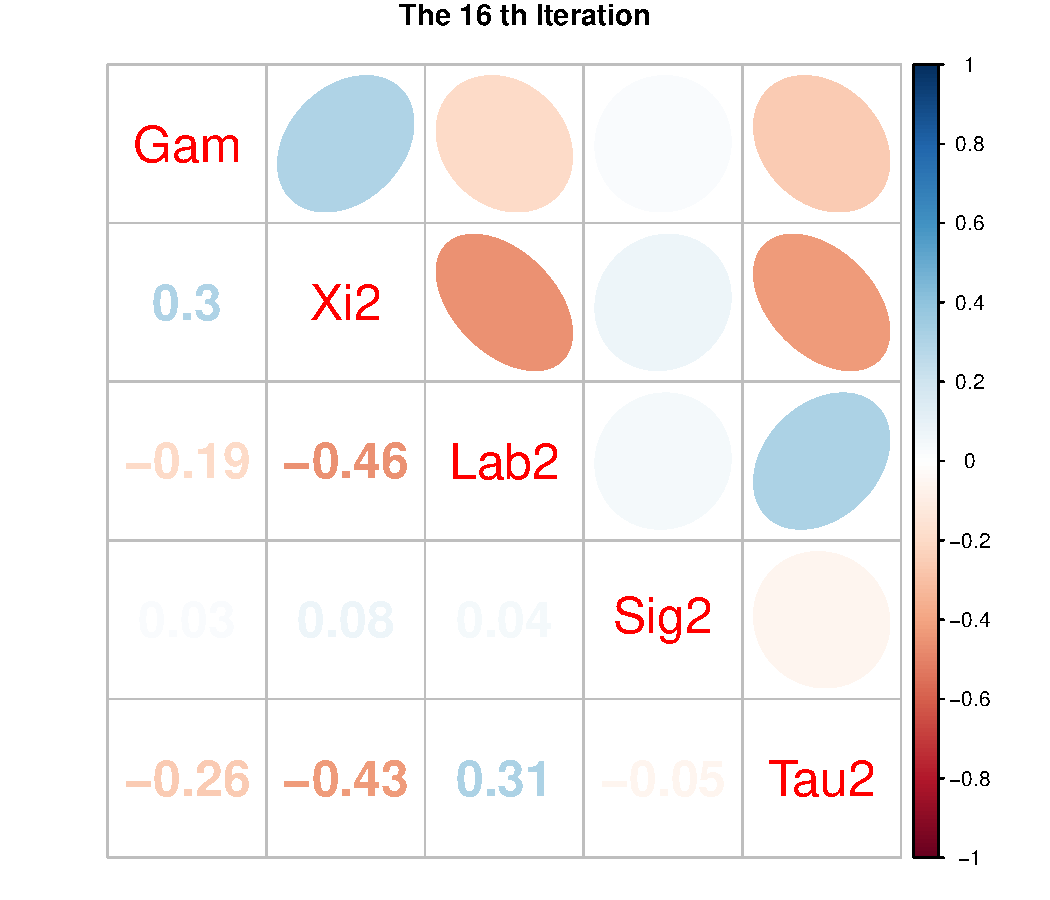
\includegraphics[width=0.3\textwidth,height=0.2\textheight]{Chapters/05MCMCOU/plots/paraEvolution/corMatrix16.pdf}
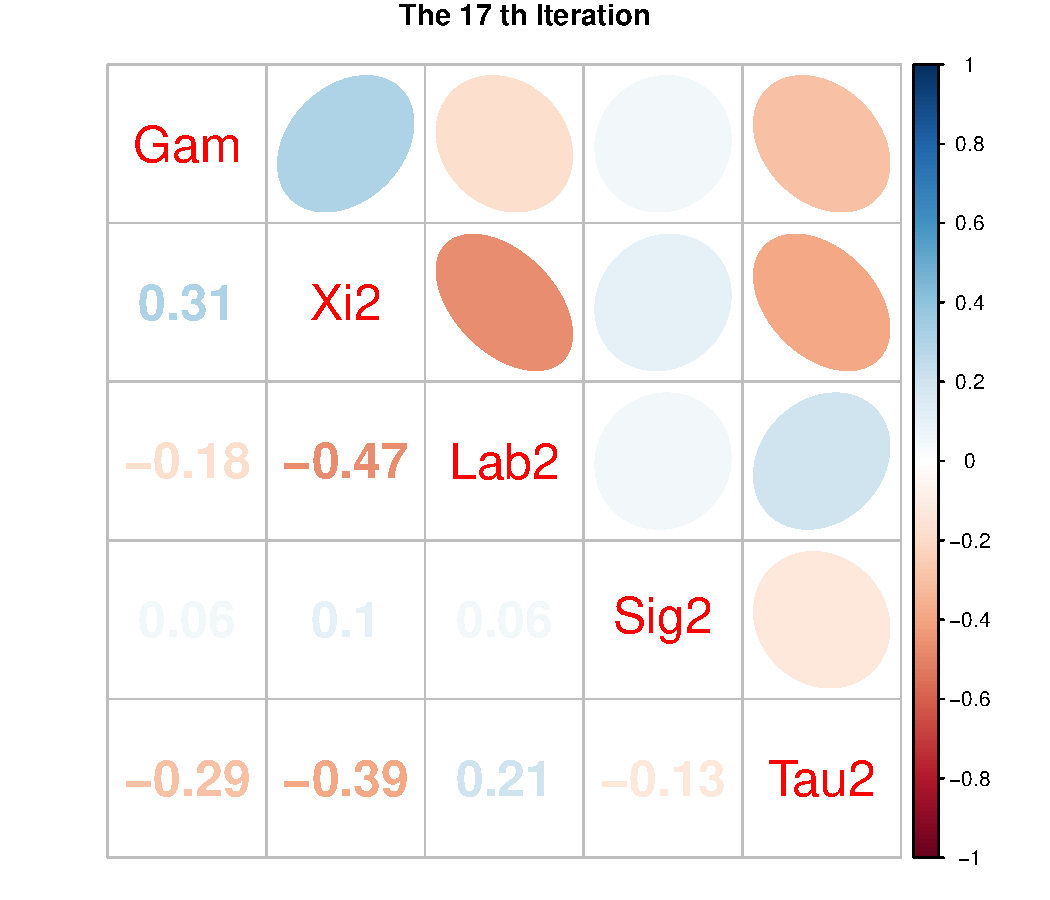
\includegraphics[width=0.3\textwidth,height=0.2\textheight]{Chapters/05MCMCOU/plots/paraEvolution/corMatrix17.pdf}
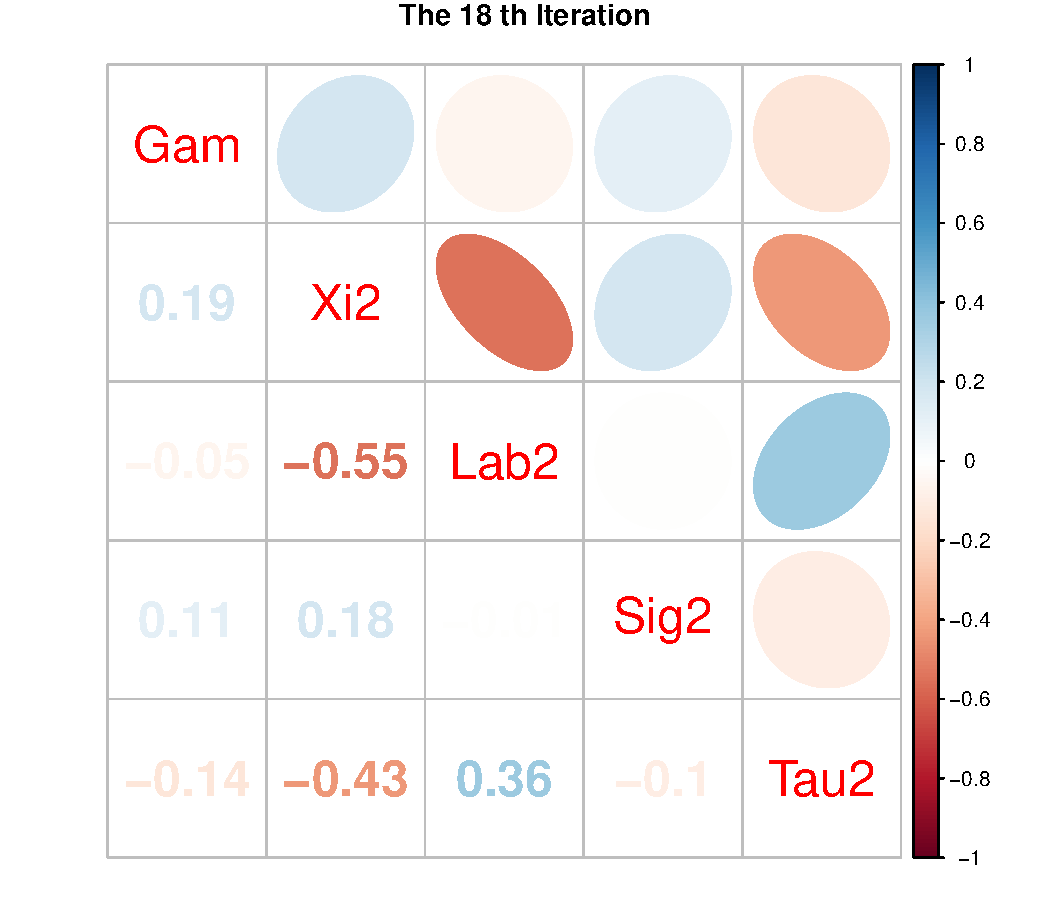
\includegraphics[width=0.3\textwidth,height=0.2\textheight]{Chapters/05MCMCOU/plots/paraEvolution/corMatrix18.pdf}
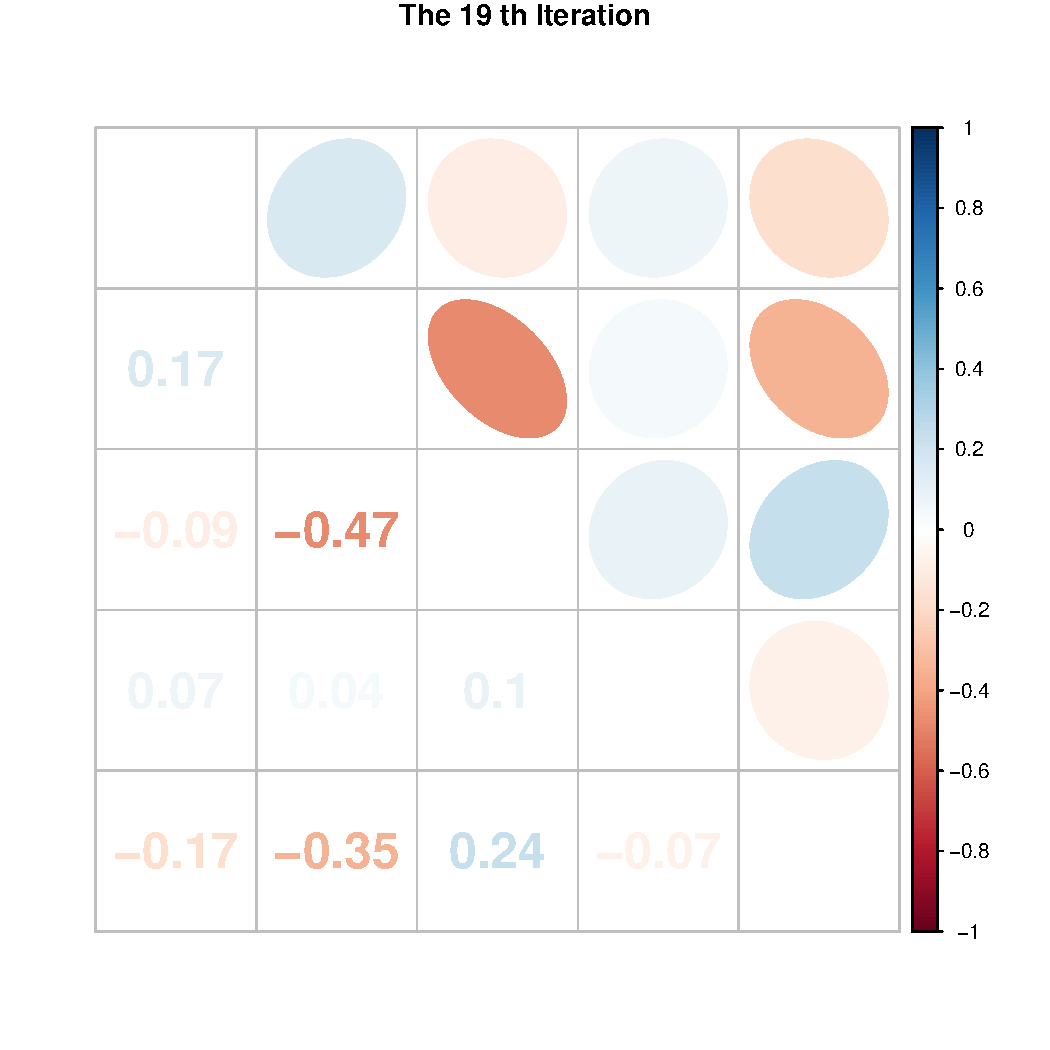
\includegraphics[width=0.3\textwidth,height=0.2\textheight]{Chapters/05MCMCOU/plots/paraEvolution/corMatrix19.pdf}
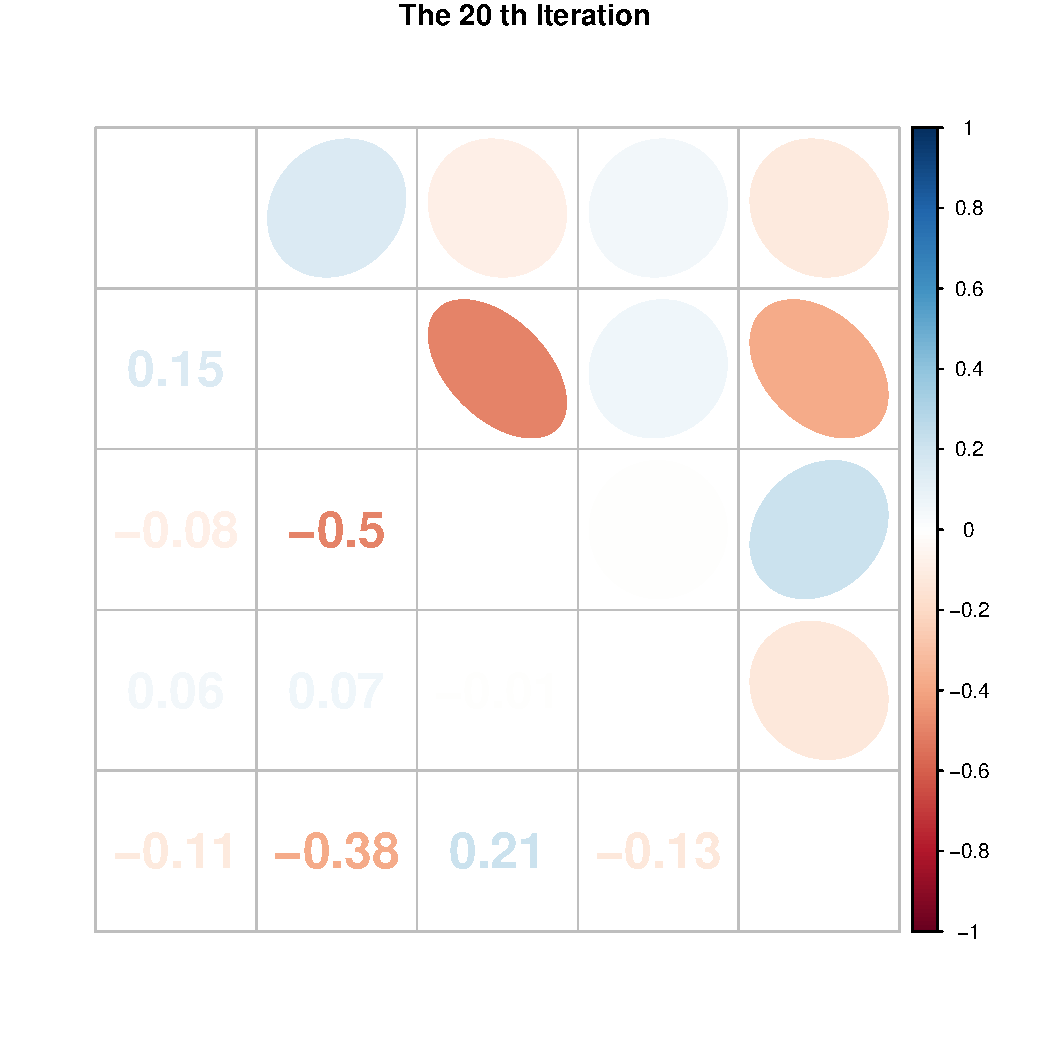
\includegraphics[width=0.3\textwidth,height=0.2\textheight]{Chapters/05MCMCOU/plots/paraEvolution/corMatrix20.pdf}
\includegraphics[width=0.3\textwidth,height=0.2\textheight]{Chapters/05MCMCOU/plots/paraEvolution/corMatrix21.pdf}
\includegraphics[width=0.3\textwidth,height=0.2\textheight]{Chapters/05MCMCOU/plots/paraEvolution/corMatrix22.pdf}
\includegraphics[width=0.3\textwidth,height=0.2\textheight]{Chapters/05MCMCOU/plots/paraEvolution/corMatrix23.pdf}
\includegraphics[width=0.3\textwidth,height=0.2\textheight]{Chapters/05MCMCOU/plots/paraEvolution/corMatrix24.pdf}
%\caption{Parameter Evolution Visualization. }
\end{figure}
\begin{figure}[h]\ContinuedFloat
\centering
\includegraphics[width=0.3\textwidth,height=0.2\textheight]{Chapters/05MCMCOU/plots/paraEvolution/corMatrix25.pdf}
\includegraphics[width=0.3\textwidth,height=0.2\textheight]{Chapters/05MCMCOU/plots/paraEvolution/corMatrix26.pdf}
\includegraphics[width=0.3\textwidth,height=0.2\textheight]{Chapters/05MCMCOU/plots/paraEvolution/corMatrix27.pdf}
\includegraphics[width=0.3\textwidth,height=0.2\textheight]{Chapters/05MCMCOU/plots/paraEvolution/corMatrix28.pdf}
\includegraphics[width=0.3\textwidth,height=0.2\textheight]{Chapters/05MCMCOU/plots/paraEvolution/corMatrix29.pdf}
\includegraphics[width=0.3\textwidth,height=0.2\textheight]{Chapters/05MCMCOU/plots/paraEvolution/corMatrix30.pdf}
\includegraphics[width=0.3\textwidth,height=0.2\textheight]{Chapters/05MCMCOU/plots/paraEvolution/corMatrix31.pdf}
\includegraphics[width=0.3\textwidth,height=0.2\textheight]{Chapters/05MCMCOU/plots/paraEvolution/corMatrix32.pdf}
\includegraphics[width=0.3\textwidth,height=0.2\textheight]{Chapters/05MCMCOU/plots/paraEvolution/corMatrix33.pdf}
\includegraphics[width=0.3\textwidth,height=0.2\textheight]{Chapters/05MCMCOU/plots/paraEvolution/corMatrix34.pdf}
\includegraphics[width=0.3\textwidth,height=0.2\textheight]{Chapters/05MCMCOU/plots/paraEvolution/corMatrix35.pdf}
\includegraphics[width=0.3\textwidth,height=0.2\textheight]{Chapters/05MCMCOU/plots/paraEvolution/corMatrix36.pdf}
%\caption{Parameter Evolution Visualization. }
\end{figure}
\begin{figure}[h]\ContinuedFloat
\centering
\includegraphics[width=0.3\textwidth,height=0.2\textheight]{Chapters/05MCMCOU/plots/paraEvolution/corMatrix37.pdf}
\includegraphics[width=0.3\textwidth,height=0.2\textheight]{Chapters/05MCMCOU/plots/paraEvolution/corMatrix38.pdf}
\includegraphics[width=0.3\textwidth,height=0.2\textheight]{Chapters/05MCMCOU/plots/paraEvolution/corMatrix39.pdf}
\includegraphics[width=0.3\textwidth,height=0.2\textheight]{Chapters/05MCMCOU/plots/paraEvolution/corMatrix40.pdf}
\includegraphics[width=0.3\textwidth,height=0.2\textheight]{Chapters/05MCMCOU/plots/paraEvolution/corMatrix41.pdf}
\includegraphics[width=0.3\textwidth,height=0.2\textheight]{Chapters/05MCMCOU/plots/paraEvolution/corMatrix42.pdf}
\includegraphics[width=0.3\textwidth,height=0.2\textheight]{Chapters/05MCMCOU/plots/paraEvolution/corMatrix42.pdf}
\includegraphics[width=0.3\textwidth,height=0.2\textheight]{Chapters/05MCMCOU/plots/paraEvolution/corMatrix44.pdf}
\includegraphics[width=0.3\textwidth,height=0.2\textheight]{Chapters/05MCMCOU/plots/paraEvolution/corMatrix45.pdf}
\includegraphics[width=0.3\textwidth,height=0.2\textheight]{Chapters/05MCMCOU/plots/paraEvolution/corMatrix46.pdf}
\includegraphics[width=0.3\textwidth,height=0.2\textheight]{Chapters/05MCMCOU/plots/paraEvolution/corMatrix47.pdf}
\includegraphics[width=0.3\textwidth,height=0.2\textheight]{Chapters/05MCMCOU/plots/paraEvolution/corMatrix48.pdf}
\caption{Parameter Evolution Visualization. The correlation among parameters does not change two much. The parameters are considered static. }
\end{figure}
